% =============================================================================
% CHAPITRE 1 - CINÉMATIQUE
% Fichier maître du chapitre
% =============================================================================

% Le \chapter est déclaré dans sec-position.tex

% 1. Définition des variables
% =============================================================================
% CHAPITRE 1 - CINÉMATIQUE
% Partie 1 : Introduction, position et déplacement
% Version maritime pour l'IMQ
% =============================================================================

\chapter{Cinématique}

% =============================================================================
\section{Introduction : qu'est-ce que la cinématique?}
% =============================================================================

La \textbf{cinématique} est la branche de la mécanique qui se consacre à la \textbf{description du mouvement} des corps. Cette description peut être :

\begin{itemize}
    \item \textbf{Qualitative} : « Le navire s'approche du quai en ralentissant. »
    \item \textbf{Math\'ematique} : \guillemotleft~Le navire se d\'eplace \`a $\SI{5}{n\oe{}uds}$ avec une d\'ec\'el\'eration\footnote{En physique, la \textit{d\'ec\'el\'eration} correspond simplement \`a une acc\'el\'eration dont le vecteur est oppos\'e au vecteur vitesse. On parle aussi d'\textit{acc\'el\'eration n\'egative}.} de $\SI{0,2}{m/s^2}$.~\guillemotright
\end{itemize}

\begin{attention}[title=Ce que la cinématique ne fait PAS]
La cinématique \textbf{décrit} le mouvement, mais elle ne cherche pas à l'\textbf{expliquer}. Les questions comme « Pourquoi le navire accélère-t-il? » ou « Quelle force est nécessaire pour freiner? » relèvent de la \textbf{dynamique}, que nous étudierons au chapitre suivant.

En cinématique, on répond aux questions : \textit{Où? Quand? À quelle vitesse? Avec quelle accélération?}
\end{attention}

Pour décrire complètement un mouvement, la cinématique utilise trois grandeurs fondamentales :
\begin{enumerate}
    \item La \textbf{position} (et le \textbf{déplacement})
    \item La \textbf{vitesse}
    \item L'\textbf{accélération}
\end{enumerate}

Ces grandeurs sont reliées entre elles et dépendent toutes du \textbf{temps}. La description cinématique peut se faire de plusieurs façons : par des \textbf{équations mathématiques}, par des \textbf{graphiques} ou par des \textbf{tableaux de valeurs}.

\begin{remarque}[title=La cinématique dans le contexte maritime]
Pour un officier de navigation, la cinématique est omniprésente :
\begin{itemize}
    \item Calculer le temps d'arrivée à partir de la vitesse et de la distance
    \item Prévoir la distance de freinage lors d'une man\oe{}uvre d'accostage
    \item Estimer la trajectoire d'un navire en approche pour éviter une collision
    \item Planifier une man\oe{}uvre d'homme à la mer
\end{itemize}
La maîtrise de ces concepts vous permettra de prendre des décisions éclairées en mer.
\end{remarque}

\begin{remarque}[title=L'universalité de la cinématique]
Les concepts de la cinématique sont \textbf{universels} : ils s'appliquent aussi bien à un navire qu'à une voiture, un avion, un ballon de soccer ou même une molécule. Les mêmes équations décrivent le mouvement d'un pétrolier de 300 000 tonnes et celui d'un électron dans un fil électrique!

Dans ce cours, nous utiliserons principalement des exemples maritimes, mais gardez en tête que ces principes s'appliquent à \textbf{tout objet en mouvement}.
\end{remarque}

\subsection{Le modèle de la particule}

L'observation de phénomènes physiques nous permet de constater qu'un mouvement correspond à une variation continue de la position d'un objet. Néanmoins, il est parfois possible de simplifier l'étude de ces mouvements en négligeant les dimensions de l'objet.

\begin{definition}[title=Modèle de la particule]
Lorsqu'on ne tient pas compte des dimensions d'un objet et qu'on néglige sa rotation sur lui-même, on peut considérer que toute sa masse est concentrée en un point unique : son \textbf{centre de masse}. L'objet est alors traité comme une \textbf{particule}.
\end{definition}

\begin{exemple}{Quand utiliser le modèle de la particule?}{}
Un vraquier de $\SI{200}{m}$ de long navigue en haute mer à $\SI{12}{n\oe{}uds}$. Pour calculer son temps de traversée sur une distance de $\SI{500}{milles nautiques}$, on peut traiter le navire comme une particule : ses dimensions ($\SI{200}{m}$) sont négligeables par rapport à la distance parcourue ($\SI{926}{km}$).

Par contre, pour une manœuvre d'accostage, les dimensions du navire deviennent importantes et le modèle de la particule n'est plus approprié.
\end{exemple}

% =============================================================================
\section{Position et déplacement}
% =============================================================================

\subsection{Système de référence}

Pour décrire le mouvement d'un objet, il faut d'abord établir un \textbf{système de référence} (ou référentiel) composé de :
\begin{itemize}
    \item Un \textbf{point d'origine} O
    \item Un ou plusieurs \textbf{axes orientés} (un axe en 1D, deux axes en 2D, trois axes en 3D)
    \item Une \textbf{unité de mesure} (généralement le mètre)
\end{itemize}

En navigation, on travaille généralement en \textbf{deux dimensions} (la surface de l'eau). Nous utiliserons donc un système d'axes $x$ et $y$ perpendiculaires.

\begin{remarque}[title=Le choix de l'origine est arbitraire]
Le choix du point d'origine est \textbf{complètement arbitraire} et peut être modifié selon le problème. Par exemple :
\begin{itemize}
    \item Pour une man\oe{}uvre d'accostage, on peut placer l'origine \textbf{au quai} (ainsi $x = 0$ correspond à l'objectif)
    \item Pour une traversée, on peut placer l'origine \textbf{au port de départ}
    \item Pour un problème de collision, on peut placer l'origine \textbf{sur l'un des navires}
\end{itemize}

Un bon choix d'origine peut \textbf{simplifier considérablement} les calculs. N'hésitez pas à repositionner l'origine selon ce qui rend le problème plus simple!

\textbf{Important :} Quelle que soit l'origine choisie, les \textbf{grandeurs physiques} (déplacement, vitesse, accélération) restent les mêmes. Seules les \textbf{coordonnées} changent.
\end{remarque}

\begin{center}
\begin{tikzpicture}[scale=0.9]
% Fond de carte (mer)
\fill[blue!10] (-1,-1) rectangle (8,6);
% Axes
\draw[axe, very thick, ->] (0,0) -- (7.5,0) node[right] {$x$ (Est)};
\draw[axe, very thick, ->] (0,0) -- (0,5.5) node[above] {$y$ (Nord)};
% Origine
\fill (0,0) circle (3pt);
\node[below left] at (0,0) {O (origine)};
% Graduations
\foreach \x in {1,2,3,4,5,6,7} {
    \draw (\x,0.1) -- (\x,-0.1) node[below] {\small \x};
}
\foreach \y in {1,2,3,4,5} {
    \draw (0.1,\y) -- (-0.1,\y) node[left] {\small \y};
}
% Point P
\fill[red] (5,3) circle (4pt);
\node[above right] at (5,3) {P};
% Vecteur position
\draw[vecteur rouge, very thick] (0,0) -- (5,3) node[midway, above left] {$\vect{r}$};
% Composantes
\draw[dashed, gray] (5,0) -- (5,3);
\draw[dashed, gray] (0,3) -- (5,3);
% Annotations composantes
\draw[thick, blue, ->] (0,0) -- (5,0) node[midway, below] {$x = 5$};
\draw[thick, green!60!black, ->] (5,0) -- (5,3) node[midway, right] {$y = 3$};
\end{tikzpicture}
\end{center}

\subsection{Vecteur position}

\begin{definition}[title=Vecteur position]
Le \textbf{vecteur position} $\vect{r}$ d'une particule est le vecteur qui va de l'origine O du système de référence jusqu'à la position de la particule.

En deux dimensions, le vecteur position est caractérisé par ses \textbf{deux composantes} :
\begin{equationimportante}
\begin{equation}
\vect{r} = (x, y)
\end{equation}
\end{equationimportante}
où $x$ est la coordonnée horizontale et $y$ est la coordonnée verticale.

L'unité SI de la position est le \textbf{mètre} (m).
\end{definition}

\begin{remarque}[title=Module du vecteur position]
Le \textbf{module} (ou norme) du vecteur position représente la distance entre l'origine et la particule :
\[ |\vect{r}| = \sqrt{x^2 + y^2} \]
\end{remarque}

\begin{exemple}{Position d'un navire en mer}{}
Un navire se trouve à $\SI{4}{km}$ à l'est et $\SI{3}{km}$ au nord d'un phare pris comme origine.

\textbf{Vecteur position :}
\[ \vect{r} = (\SI{4}{km}, \SI{3}{km}) \]

\textbf{Distance au phare :}
\[ |\vect{r}| = \sqrt{4^2 + 3^2} = \sqrt{16 + 9} = \sqrt{25} = \SI{5}{km} \]

\begin{center}
\begin{tikzpicture}[scale=0.8]
% Mer
\fill[blue!10] (-0.5,-0.5) rectangle (6,5);
% Axes
\draw[axe, thick, ->] (0,0) -- (5.5,0) node[right] {Est (km)};
\draw[axe, thick, ->] (0,0) -- (0,4.5) node[above] {Nord (km)};
% Phare
\fill[orange] (0,0) circle (5pt);
\node[below left] at (0,0) {Phare};
% Navire
\fill[blue!70!black] (4,3) circle (4pt);
\node[above right] at (4,3) {Navire};
% Vecteur position
\draw[vecteur rouge, very thick] (0,0) -- (4,3);
\node[red] at (1.5,2) {$\vect{r}$};
% Composantes
\draw[dashed, gray] (4,0) -- (4,3);
\draw[dashed, gray] (0,3) -- (4,3);
\node[below] at (2,0) {$x = \SI{4}{km}$};
\node[left] at (0,1.5) {$y = \SI{3}{km}$};
% Distance
\node[red, right] at (2.5,1) {$|\vect{r}| = \SI{5}{km}$};
\end{tikzpicture}
\end{center}
\end{exemple}

\subsection{Cas particulier : mouvement en une dimension}

Lorsque le mouvement se fait le long d'une seule direction (par exemple, un navire dans un chenal rectiligne), on peut simplifier en utilisant \textbf{un seul axe}. La position devient alors un simple nombre algébrique $x$ (positif ou négatif selon le côté de l'origine).

\begin{exemple}{Position d'un navire dans un chenal}{}
Un chenal maritime est balisé par des bouées. On établit l'origine au niveau de la bouée d'entrée, avec l'axe $x$ positif vers l'intérieur du port.

\begin{center}
\begin{tikzpicture}[scale=0.8]
% Axe
\draw[axe, thick] (-1,0) -- (10,0) node[right] {$x$ (m)};
% Origine
\fill (0,0) circle (3pt) node[below=5pt] {$0$};
\node[above] at (0,0.3) {Bouée d'entrée};
% Graduations
\foreach \x in {2,4,6,8} {
    \draw (\x,0.1) -- (\x,-0.1) node[below] {$\x 00$};
}
% Navire
\node[above] at (5,0.5) {\textbf{Navire}};
\draw[thick, blue] (4.5,0.3) -- (5.5,0.3) -- (5.7,0.5) -- (5.5,0.7) -- (4.5,0.7) -- cycle;
\draw[vecteur rouge] (0,0.5) -- (5,0.5) node[midway, above] {$x = \SI{500}{m}$};
\end{tikzpicture}
\end{center}

La position du navire est $x = \SI{+500}{m}$ (positif car dans le sens de l'axe).
\end{exemple}

\subsection{Vecteur déplacement}

\begin{definition}[title=Vecteur déplacement]
Le \textbf{vecteur déplacement} $\Delta\vect{r}$ est la variation du vecteur position entre deux instants. C'est le vecteur qui va de la position initiale à la position finale :
\begin{equationimportante}
\begin{equation}
\Delta\vect{r} = \vect{r}_f - \vect{r}_i
\end{equation}
\end{equationimportante}

En composantes, cela donne :
\begin{equationimportante}
\begin{align}
\Delta\vect{r} &= (\Delta x, \Delta y) \\[0.3cm]
\text{où} \quad \Delta x &= x_f - x_i \quad \text{et} \quad \Delta y = y_f - y_i
\end{align}
\end{equationimportante}
\end{definition}

\begin{remarque}[title=Module du déplacement]
Le \textbf{module du déplacement} représente la distance en ligne droite entre la position initiale et la position finale :
\[ |\Delta\vect{r}| = \sqrt{(\Delta x)^2 + (\Delta y)^2} \]
\end{remarque}

\begin{exemple}{Déplacement d'un cargo entre deux ports}{}
Un cargo quitte Rimouski (position initiale) pour se rendre à Sept-Îles (position finale). En prenant Rimouski comme origine :
\begin{itemize}
    \item Position initiale : $\vect{r}_i = (\SI{0}{km}, \SI{0}{km})$
    \item Position finale : $\vect{r}_f = (\SI{280}{km}, \SI{95}{km})$ (Sept-Îles est à l'est-nord-est)
\end{itemize}

\begin{center}
\begin{tikzpicture}[scale=0.022]
% Mer
\fill[blue!10] (-20,-20) rectangle (320,140);
% Côte schématique
\fill[brown!20] (-20,-20) -- (-20,30) -- (50,10) -- (100,25) -- (150,15) -- (200,40) -- (280,80) -- (320,75) -- (320,-20) -- cycle;
% Axes
\draw[axe, thick, ->] (0,0) -- (310,0) node[right] {$x$ (km)};
\draw[axe, thick, ->] (0,0) -- (0,130) node[above] {$y$ (km)};
% Graduations
\foreach \x in {100,200,300} {
    \draw (\x,3) -- (\x,-3) node[below] {\small \x};
}
\foreach \y in {50,100} {
    \draw (3,\y) -- (-3,\y) node[left] {\small \y};
}
% Rimouski
\fill[red] (0,0) circle (8pt);
\node[below left] at (0,0) {\textbf{Rimouski}};
% Sept-Îles
\fill[red] (280,95) circle (8pt);
\node[above right] at (280,95) {\textbf{Sept-Îles}};
% Vecteur déplacement
\draw[vecteur rouge, very thick] (0,0) -- (280,95);
\node[red] at (120,70) {$\Delta\vect{r}$};
% Composantes
\draw[dashed, blue, thick] (0,0) -- (280,0) node[midway, below] {$\Delta x = \SI{280}{km}$};
\draw[dashed, green!60!black, thick] (280,0) -- (280,95) node[midway, right] {$\Delta y = \SI{95}{km}$};
\end{tikzpicture}
\end{center}

\textbf{Vecteur déplacement :}
\[ \Delta\vect{r} = \vect{r}_f - \vect{r}_i = (280 - 0, 95 - 0) = (\SI{280}{km}, \SI{95}{km}) \]

\textbf{Module du déplacement} (distance en ligne droite) :
\[ |\Delta\vect{r}| = \sqrt{280^2 + 95^2} = \sqrt{78400 + 9025} = \sqrt{87425} \approx \SI{296}{km} \]

En milles nautiques : $296 \text{ km} \times \dfrac{1 \text{ NM}}{1,852 \text{ km}} \approx \SI{160}{NM}$
\end{exemple}

\begin{pratiqueautonome}
Un navire de recherche part d'une plateforme pétrolière située à l'origine et effectue deux déplacements successifs :
\begin{itemize}
    \item Premier déplacement : $\SI{12}{km}$ vers l'est
    \item Deuxième déplacement : $\SI{5}{km}$ vers le nord
\end{itemize}

\begin{enumerate}[label=\alph*)]
    \item Écrivez le vecteur déplacement total en composantes : $\Delta\vect{r} = (\Delta x, \Delta y)$
    \item Calculez le module du déplacement total $|\Delta\vect{r}|$.
    \item Quelle est la distance totale parcourue $d$?
\end{enumerate}

\espaceresolution[5cm]
\reponsepratique{a) $\Delta\vect{r} = (\SI{12}{km}, \SI{5}{km})$ \quad b) $|\Delta\vect{r}| = \SI{13}{km}$ \quad c) $d = \SI{17}{km}$}
\end{pratiqueautonome}

\subsection{Déplacement vs distance parcourue}

\begin{attention}[title=Ne jamais confondre ces deux grandeurs!]
\begin{center}
\renewcommand{\arraystretch}{1.4}
\begin{tabular}{|L{6cm}|L{6cm}|}
\hline
\rowcolor{bleuclair}
\textbf{Déplacement} $\Delta\vect{r}$ & \textbf{Distance parcourue} $d$ \\
\hline
Dépend uniquement des positions initiale et finale & Dépend du trajet emprunté \\
\hline
Grandeur \textbf{vectorielle} (a une direction) & Grandeur \textbf{scalaire} (pas de direction) \\
\hline
Le module peut être nul même si l'objet a bougé & Toujours positive ou nulle \\
\hline
$|\Delta\vect{r}| = \sqrt{(\Delta x)^2 + (\Delta y)^2}$ & $d \geq |\Delta\vect{r}|$ toujours \\
\hline
\end{tabular}
\end{center}
\end{attention}

\begin{definition}[title=Distance parcourue]
La \textbf{distance parcourue} $d$ est la longueur totale du trajet suivi par l'objet, mesurée le long de sa trajectoire.

\begin{itemize}
    \item C'est une grandeur \textbf{scalaire} (toujours positive ou nulle)
    \item Elle ne contient aucune information sur la direction
    \item Elle est toujours supérieure ou égale au module du déplacement : $d \geq |\Delta\vect{r}|$
    \item L'égalité $d = |\Delta\vect{r}|$ n'est vraie que si le mouvement est en ligne droite \textbf{sans demi-tour}
\end{itemize}
\end{definition}

\begin{exemple}{Manœuvre d'un remorqueur (cas 1D)}{}
Un remorqueur effectue une manœuvre dans un port. Il part du quai A (position $x_i = \SI{0}{m}$), se rend au quai B (position $x = \SI{800}{m}$), puis revient au quai C (position $x_f = \SI{300}{m}$).

\begin{center}
\begin{tikzpicture}[scale=0.7]
% Axe
\draw[axe, thick] (-0.5,0) -- (10,0) node[right] {$x$ (m)};
% Points
\fill (0,0) circle (3pt) node[below=5pt] {A ($0$)};
\fill (8,0) circle (3pt) node[below=5pt] {B ($800$)};
\fill (3,0) circle (3pt) node[below=5pt] {C ($300$)};
% Trajets
\draw[->, thick, blue] (0,0.5) -- (8,0.5) node[midway, above] {$\SI{800}{m}$};
\draw[->, thick, red] (8,1.2) -- (3,1.2) node[midway, above] {$\SI{500}{m}$};
\end{tikzpicture}
\end{center}

\textbf{Distance parcourue :}
\[ d = \SI{800}{m} + \SI{500}{m} = \SI{1300}{m} \]

\textbf{Déplacement :}
\[ \Delta x = x_f - x_i = \SI{300}{m} - \SI{0}{m} = \SI{+300}{m} \]

Le déplacement ne représente que le changement \textit{net} de position, peu importe le trajet.
\end{exemple}

\begin{pratiqueautonome}
Un traversier part du quai A (position $x_i = \SI{0}{m}$), se rend à la bouée B située à $x = \SI{600}{m}$, puis continue jusqu'au quai C situé à $x = \SI{200}{m}$.

\begin{enumerate}[label=\alph*)]
    \item Calculez le déplacement total $\Delta x$.
    \item Calculez la distance parcourue $d$.
\end{enumerate}

\espaceresolution[5cm]
\reponsepratique{a) $\Delta x = +\SI{200}{m}$ \quad b) $d = \SI{1000}{m}$}
\end{pratiqueautonome}

\begin{exemple}{Patrouille maritime -- trajectoire fermée (cas 2D)}{}
Un patrouilleur des garde-côtes part de sa base (point B), effectue une ronde de surveillance autour d'une zone de pêche en passant par les points P1, P2 et P3, puis revient à sa base après $\SI{4}{heures}$.

\begin{center}
\begin{tikzpicture}[scale=0.9]
% Fond de carte (mer)
\fill[blue!10] (-1,-1) rectangle (8,6);
% Axes
\draw[axe, thick, ->] (-0.5,0) -- (7.5,0) node[right] {$x$ (NM)};
\draw[axe, thick, ->] (0,-0.5) -- (0,5.5) node[above] {$y$ (NM)};
% Côte
\fill[brown!30] (-1,-1) -- (-1,2) -- (0,1.5) -- (0.5,2) -- (0,-1) -- cycle;
\draw[thick, brown!60!black] (-1,2) -- (0,1.5) -- (0.5,2);
% Base
\fill[red!70!black] (0.3,1) circle (4pt);
\node[left] at (0,1) {\textbf{Base (B)}};
\node[below right] at (0.3,0.8) {\small $(0,3; 1)$};
% Points de passage
\fill[blue!70!black] (3,4) circle (3pt) node[above] {P1};
\fill[blue!70!black] (6,3) circle (3pt) node[right] {P2};
\fill[blue!70!black] (5,0.5) circle (3pt) node[below] {P3};
% Trajectoire
\draw[very thick, blue!70!black, ->] (0.3,1) -- (3,4);
\draw[very thick, blue!70!black, ->] (3,4) -- (6,3);
\draw[very thick, blue!70!black, ->] (6,3) -- (5,0.5);
\draw[very thick, blue!70!black, ->] (5,0.5) -- (0.3,1);
% Distances
\node[blue!50!black] at (1.3,2.8) {\small 15 NM};
\node[blue!50!black] at (4.8,3.8) {\small 12 NM};
\node[blue!50!black] at (6,1.5) {\small 10 NM};
\node[blue!50!black] at (2.5,0.3) {\small 11 NM};
% Zone de pêche (cercle en pointillés)
\draw[dashed, orange, thick] (4,2.5) circle (1.8);
\node[orange] at (4,2.5) {\small Zone de pêche};
\end{tikzpicture}
\end{center}

\textbf{Distance parcourue :} 
\[ d = \SI{15}{NM} + \SI{12}{NM} + \SI{10}{NM} + \SI{11}{NM} = \SI{48}{NM} \]

\textbf{Déplacement :} 

Position initiale = Position finale (retour à la base), donc :
\[ \Delta\vect{r} = \vect{r}_f - \vect{r}_i = \vect{0} \quad \Rightarrow \quad |\Delta\vect{r}| = \SI{0}{NM} \]

\begin{attention}
Ce résultat illustre une différence fondamentale :
\begin{itemize}
    \item La \textbf{distance parcourue} ($\SI{48}{NM}$) reflète l'effort réel du patrouilleur (carburant consommé, temps de navigation)
    \item Le \textbf{déplacement} (nul) indique seulement que le navire est revenu à son point de départ
\end{itemize}
Ces deux grandeurs répondent à des questions différentes!
\end{attention}
\end{exemple}

% =============================================================================
% CHAPITRE 1 - CINÉMATIQUE
% Partie 2 : La vitesse (toutes les définitions)
% Version maritime pour l'IMQ
% =============================================================================

% =============================================================================
\section{La vitesse}
% =============================================================================

\subsection{Importance de la vitesse}

La vitesse est l'une des grandeurs les plus fondamentales en physique. Elle quantifie \`a quel point un objet change de position rapidement. 

\begin{remarque}[title=La vitesse dans la vie quotidienne et professionnelle]
La vitesse est omnipr\'esente dans notre monde :
\begin{itemize}
    \item Un \textbf{conducteur} surveille son indicateur de vitesse pour respecter les limites
    \item Un \textbf{athl\`ete} cherche \`a optimiser sa vitesse de course ou de nage
    \item Un \textbf{pilote d'avion} doit maintenir une vitesse minimale pour ne pas d\'ecrocher
    \item Un \textbf{m\'edecin} mesure la vitesse de conduction nerveuse ou la vitesse du sang
    \item Un \textbf{officier de navigation} calcule les temps de travers\'ee, planifie les man\oe{}uvres et anticipe les situations de collision
\end{itemize}

Dans le contexte maritime, la vitesse est une donn\'ee critique : elle d\'etermine le temps d'arriv\'ee, la consommation de carburant, et la s\'ecurit\'e des man\oe{}uvres.
\end{remarque}

\subsection{Plusieurs d\'efinitions de la vitesse}

\begin{attention}[title=La vitesse n'est pas une seule chose!]
En physique, le mot \guillemotleft~vitesse~\guillemotright{} recouvre \textbf{plusieurs concepts distincts} :
\begin{itemize}
    \item La \textbf{vitesse scalaire moyenne} : quelle distance par unit\'e de temps?
    \item La \textbf{vitesse moyenne} : quel d\'eplacement par unit\'e de temps? (orient\'ee)
    \item La \textbf{vitesse instantan\'ee} : quelle vitesse \`a un instant pr\'ecis?
\end{itemize}

Ces trois d\'efinitions ne donnent \textbf{pas la m\^eme information}. Il est crucial de savoir laquelle utiliser selon le contexte.
\end{attention}

Commen\c{c}ons par la plus simple : la vitesse scalaire moyenne.

% =============================================================================
\subsection{Vitesse scalaire moyenne}
% =============================================================================

\begin{definition}[title=Vitesse scalaire moyenne]
La \textbf{vitesse scalaire moyenne} est le rapport entre la \textbf{distance totale parcourue} et l'intervalle de temps :
\begin{equationimportante}
\begin{equation}
v_{scalaire} = \frac{\text{distance parcourue}}{\Delta t} = \frac{d}{\Delta t}
\end{equation}
\end{equationimportante}

\begin{itemize}
    \item L'unit\'e SI est le \textbf{m\`etre par seconde} (\si{m/s})
    \item La vitesse scalaire moyenne est \textbf{toujours positive ou nulle}
    \item Elle repr\'esente l'\guillemotleft~effort r\'eel~\guillemotright{} de d\'eplacement
\end{itemize}
\end{definition}

\begin{remarque}[title=Unit\'es de vitesse courantes]
\begin{center}
\renewcommand{\arraystretch}{1.3}
\begin{tabular}{|l|l|}
\hline
\rowcolor{bleuclair}
\textbf{Unit\'e} & \textbf{\'Equivalence} \\
\hline
$\SI{1}{m/s}$ & Unit\'e SI de r\'ef\'erence \\
\hline
$\SI{1}{km/h}$ & $= \SI{0,278}{m/s} = \frac{1}{3,6}\,\si{m/s}$ \\
\hline
$\SI{1}{n\oe{}ud}$ (nd ou kn) & $= \SI{1,852}{km/h} = \SI{0,5144}{m/s}$ \\
\hline
\end{tabular}
\end{center}

Le \textbf{n\oe{}ud} est l'unit\'e de vitesse en navigation : $\SI{1}{n\oe{}ud} = \SI{1}{mille nautique/heure}$.
\end{remarque}

\begin{exemple}{Man\oe{}uvre d'un remorqueur}{}
Un remorqueur part du quai A, se rend au quai B ($\SI{800}{m}$), puis revient au quai C ($\SI{500}{m}$ de recul). La man\oe{}uvre totale prend $\SI{20}{minutes}$.

\textbf{Donn\'ees :}
\begin{itemize}
    \item Distance parcourue : $d = \SI{800}{m} + \SI{500}{m} = \SI{1300}{m}$
    \item Temps : $\Delta t = \SI{20}{min} \times \dfrac{\SI{60}{s}}{\SI{1}{min}} = \SI{1200}{s}$
\end{itemize}

\textbf{Vitesse scalaire moyenne :}
\[ v_{scalaire} = \frac{d}{\Delta t} = \frac{\SI{1300}{m}}{\SI{1200}{s}} = \SI{1,08}{m/s} \]

Conversion en n\oe{}uds :
\[ v_{scalaire} = \SI{1,08}{m/s} \times \frac{\SI{1}{n\oe{}ud}}{\SI{0,5144}{m/s}} = \SI{2,1}{n\oe{}uds} \]

Cette valeur repr\'esente bien l'activit\'e r\'eelle du remorqueur pendant ces 20 minutes.
\end{exemple}

% =============================================================================
\subsection{Vitesse moyenne}
% =============================================================================

La vitesse scalaire moyenne ne contient aucune information sur la \textbf{direction} du mouvement. Pour cela, on d\'efinit la vitesse moyenne.

\begin{definition}[title=Vitesse moyenne]
La \textbf{vitesse moyenne} $v_{moy}$ d'un objet est le rapport entre son \textbf{d\'eplacement} et l'intervalle de temps correspondant :
\begin{equationimportante}
\begin{equation}
v_{moy} = \frac{\Delta x}{\Delta t} = \frac{x_f - x_i}{t_f - t_i}
\end{equation}
\end{equationimportante}

\begin{itemize}
    \item C'est une grandeur \textbf{vectorielle} (en 1D : elle a un signe)
    \item Elle peut \^etre positive, n\'egative ou nulle
    \item Elle indique la \textbf{direction} du mouvement net
\end{itemize}
\end{definition}

\begin{remarque}[title=Signe de la vitesse moyenne]
Puisque $\Delta t$ est toujours positif, le \textbf{signe de la vitesse moyenne} est le m\^eme que celui du d\'eplacement :
\begin{itemize}
    \item $v_{moy} > 0$ : mouvement net dans le sens positif de l'axe
    \item $v_{moy} < 0$ : mouvement net dans le sens n\'egatif de l'axe
    \item $v_{moy} = 0$ : retour au point de d\'epart (d\'eplacement nul)
\end{itemize}
\end{remarque}

\begin{exemple}{Travers\'ee maritime}{}
Un cargo quitte le port de Rimouski \`a 8h00 et arrive \`a Sept-\^Iles \`a 20h00. La distance directe (d\'eplacement) entre les deux ports est de $\SI{180}{milles nautiques}$ vers l'est.

\textbf{Solution :}

Intervalle de temps : $\Delta t = 20h00 - 8h00 = \SI{12}{h}$

Vitesse moyenne :
\[ v_{moy} = \frac{\Delta x}{\Delta t} = \frac{\SI{+180}{NM}}{\SI{12}{h}} = \SI{+15}{n\oe{}uds} \]

Le signe positif indique que le mouvement est vers l'est (sens positif de l'axe).
\end{exemple}

\begin{pratiqueautonome}
Un cargo quitte le port de Matane à 6h00 et arrive à Baie-Comeau à 10h00. La distance directe entre les deux ports est de $\SI{52}{km}$ vers le nord-est.

Calculez la vitesse moyenne du cargo en km/h et en n\oe{}uds.

\espaceresolution[5cm]
\reponsepratique{$v_{moy} = \SI{13}{km/h} \approx \SI{7,0}{n\oe{}uds}$}
\end{pratiqueautonome}

\subsection{Pourquoi les deux sont importantes?}

\begin{center}
\renewcommand{\arraystretch}{1.4}
\begin{tabular}{|L{6cm}|L{6cm}|}
\hline
\rowcolor{bleuclair}
\textbf{Vitesse scalaire moyenne} $v_{scalaire}$ & \textbf{Vitesse moyenne} $v_{moy}$ \\
\hline
Bas\'ee sur la \textbf{distance parcourue} & Bas\'ee sur le \textbf{d\'eplacement} \\
\hline
Toujours positive ou nulle & Peut \^etre positive, n\'egative ou nulle \\
\hline
Repr\'esente l'\textbf{effort r\'eel} (\'energie d\'epens\'ee, carburant consomm\'e) & Repr\'esente le \textbf{r\'esultat net} (o\`u on s'est rendu) \\
\hline
N'indique pas la direction & \textbf{Indique la direction} du mouvement net \\
\hline
$v_{scalaire} = \dfrac{d}{\Delta t}$ & $v_{moy} = \dfrac{\Delta x}{\Delta t}$ \\
\hline
\end{tabular}
\end{center}

\begin{exemple}{Croisi\`ere Qu\'ebec -- \^Iles-de-la-Madeleine : comparaison}{}
Un navire de croisi\`ere quitte Qu\'ebec, fait escale aux \^Iles-de-la-Madeleine (\`a $\SI{650}{km}$), puis revient \`a Qu\'ebec. L'aller dure 2 jours et le retour dure 2 jours.

\begin{center}
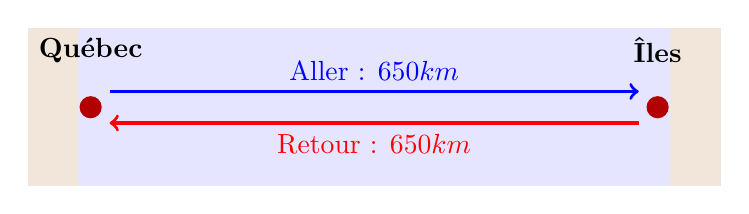
\begin{tikzpicture}[scale=0.8]
% Côte schématique
\fill[brown!20] (-0.5,-0.5) rectangle (0.3,2);
\fill[brown!20] (9.7,-0.5) rectangle (10.5,2);
% Mer
\fill[blue!10] (0.3,-0.5) rectangle (9.7,2);
% Villes
\fill[red!70!black] (0.5,0.75) circle (5pt);
\node[above] at (0.5,1.3) {\textbf{Qu\'ebec}};
\fill[red!70!black] (9.5,0.75) circle (5pt);
\node[above] at (9.5,1.3) {\textbf{\^Iles}};
% Trajets
\draw[very thick, blue, ->] (0.8,1) -- (9.2,1) node[midway, above] {Aller : $\SI{650}{km}$};
\draw[very thick, red, ->] (9.2,0.5) -- (0.8,0.5) node[midway, below] {Retour : $\SI{650}{km}$};
\end{tikzpicture}
\end{center}

\textbf{Vitesse scalaire moyenne :}
\[ v_{scalaire} = \frac{d}{\Delta t} = \frac{650 + 650}{4 \text{ jours}} = \SI{325}{km/jour} \approx \SI{13,5}{km/h} \]

\textbf{Vitesse moyenne :}
\[ v_{moy} = \frac{\Delta x}{\Delta t} = \frac{0}{4 \text{ jours}} = \SI{0}{km/h} \]

\begin{attention}
Les deux informations sont \textbf{compl\'ementaires} :
\begin{itemize}
    \item La vitesse scalaire ($\SI{13,5}{km/h}$) refl\`ete l'activit\'e r\'eelle du navire
    \item La vitesse moyenne (nulle) indique que le navire est revenu \`a son point de d\'epart
\end{itemize}
Aucune des deux n'est \guillemotleft~meilleure~\guillemotright{} --- elles r\'epondent \`a des questions diff\'erentes!
\end{attention}
\end{exemple}

\begin{exemple}{Navigation avec courant contraire}{}
Un traversier effectue l'aller-retour entre deux rives d'un fleuve s\'epar\'ees de $\SI{2}{km}$. \`A l'aller (avec le courant), il navigue \`a $\SI{12}{n\oe{}uds}$. Au retour (contre le courant), sa vitesse tombe \`a $\SI{8}{n\oe{}uds}$.

\textbf{Conversion des vitesses en km/h :}
\begin{align*}
v_{aller} &= \SI{12}{n\oe{}uds} \times \frac{\SI{1,852}{km/h}}{\SI{1}{n\oe{}ud}} = \SI{22,2}{km/h} \\[0.3cm]
v_{retour} &= \SI{8}{n\oe{}uds} \times \frac{\SI{1,852}{km/h}}{\SI{1}{n\oe{}ud}} = \SI{14,8}{km/h}
\end{align*}

\textbf{Calcul des temps :}
\begin{align*}
t_{aller} &= \frac{\SI{2}{km}}{\SI{22,2}{km/h}} = \SI{0,090}{h} = \SI{0,090}{h} \times \frac{\SI{60}{min}}{\SI{1}{h}} = \SI{5,4}{min} \\[0.3cm]
t_{retour} &= \frac{\SI{2}{km}}{\SI{14,8}{km/h}} = \SI{0,135}{h} = \SI{0,135}{h} \times \frac{\SI{60}{min}}{\SI{1}{h}} = \SI{8,1}{min}
\end{align*}

\textbf{Temps total :} $\Delta t = \SI{5,4}{min} + \SI{8,1}{min} = \SI{13,5}{min} = \SI{0,225}{h}$

\textbf{Vitesse scalaire moyenne :}
\[ v_{scalaire} = \frac{d}{\Delta t} = \frac{\SI{4}{km}}{\SI{0,225}{h}} = \SI{17,8}{km/h} = \SI{17,8}{km/h} \times \frac{\SI{1}{n\oe{}ud}}{\SI{1,852}{km/h}} = \SI{9,6}{n\oe{}uds} \]

\begin{attention}
La vitesse scalaire moyenne ($\SI{9,6}{n\oe{}uds}$) n'est \textbf{pas} la moyenne arithm\'etique des deux vitesses : $\dfrac{12 + 8}{2} = \SI{10}{n\oe{}uds}$.

C'est une erreur fr\'equente! La moyenne des vitesses ne donne la vitesse scalaire moyenne que si les \textbf{temps} de parcours sont \'egaux.
\end{attention}
\end{exemple}

\begin{pratiqueautonome}
Un remorqueur effectue un aller-retour entre deux quais séparés de $\SI{3}{km}$. À l'aller, il navigue à $\SI{10}{n\oe{}uds}$. Au retour, sa vitesse est de $\SI{6}{n\oe{}uds}$.

\begin{enumerate}[label=\alph*)]
    \item Calculez le temps total du trajet (en minutes).
    \item Calculez la vitesse scalaire moyenne. \textit{Attention au piège!}
\end{enumerate}

\espaceresolution[6cm]
\reponsepratique{a) $\Delta t \approx \SI{19,4}{min}$ \quad b) $v_{scalaire} \approx \SI{7,5}{n\oe{}uds}$ (et non $\SI{8}{n\oe{}uds}$!)}
\end{pratiqueautonome}

% =============================================================================
\subsection{Vitesse instantan\'ee}
% =============================================================================

Les vitesses moyenne et scalaire moyenne donnent une information \textbf{globale} sur un intervalle de temps. Mais que se passe-t-il \`a un \textbf{instant pr\'ecis}?

\begin{definition}[title=Vitesse instantan\'ee]
La \textbf{vitesse instantan\'ee} est la vitesse d'un objet \`a un instant pr\'ecis. C'est la vitesse moyenne calcul\'ee sur un intervalle de temps \textbf{infiniment petit} :
\begin{equationimportante}
\begin{equation}
v = \lim_{\Delta t \to 0} \frac{\Delta x}{\Delta t}
\end{equation}
\end{equationimportante}

En termes simples : c'est ce qu'affiche le \textbf{loch} (indicateur de vitesse) d'un navire ou le \textbf{compteur} d'une voiture \`a un instant donn\'e.
\end{definition}

\begin{remarque}[title=Vitesse moyenne vs vitesse instantan\'ee]
\begin{itemize}
    \item La \textbf{vitesse moyenne} caract\'erise le mouvement sur un \textbf{intervalle de temps}
    \item La \textbf{vitesse instantan\'ee} caract\'erise le mouvement \`a un \textbf{instant pr\'ecis}
    \item Si la vitesse est constante, alors $v_{instantan\'ee} = v_{moyenne}$ \`a tout instant
\end{itemize}
\end{remarque}

\begin{exemple}{Loch d'un navire}{}
Un navire acc\'el\`ere en quittant le port. Son loch affiche successivement :
\begin{itemize}
    \item \`A $t = \SI{0}{s}$ : $v = \SI{0}{n\oe{}ud}$
    \item \`A $t = \SI{60}{s}$ : $v = \SI{3}{n\oe{}uds}$
    \item \`A $t = \SI{120}{s}$ : $v = \SI{6}{n\oe{}uds}$
    \item \`A $t = \SI{180}{s}$ : $v = \SI{8}{n\oe{}uds}$
\end{itemize}

Chacune de ces valeurs est une \textbf{vitesse instantan\'ee}. La vitesse moyenne sur les 3 premi\`eres minutes n'est pas simplement $(0 + 3 + 6 + 8)/4$ --- il faudrait conna\^itre la position \`a chaque instant pour la calculer.
\end{exemple}

\begin{remarque}[title=Interpr\'etation graphique]
Sur un graphique position-temps $x(t)$, la vitesse instantan\'ee \`a un instant $t$ correspond \`a la \textbf{pente de la tangente} \`a la courbe en ce point.

Nous approfondirons cette interpr\'etation dans la section sur les graphiques.
\end{remarque}

% =============================================================================
\subsection{Vitesse surface et vitesse fond}
% =============================================================================

En navigation, on distingue deux vitesses importantes :

\begin{definition}[title=Vitesse surface et vitesse fond]
\begin{itemize}
    \item La \textbf{vitesse surface} est la vitesse du navire \textbf{par rapport \`a l'eau}. C'est ce qu'affiche le \textbf{loch}.
    \item La \textbf{vitesse fond} est la vitesse du navire \textbf{par rapport au sol}. C'est ce qu'affiche le \textbf{GPS}.
\end{itemize}

Ces deux vitesses diff\`erent lorsqu'il y a du \textbf{courant}. La relation est \textbf{vectorielle} :
\begin{equationimportante}
\begin{equation}
\vec{v}_{fond} = \vec{v}_{surface} + \vec{v}_{courant}
\end{equation}
\end{equationimportante}
\end{definition}

\begin{exemple}{Travers\'ee avec courant favorable}{}
Un navire affiche $\SI{12}{n\oe{}uds}$ au loch. Le courant de $\SI{2}{n\oe{}uds}$ pousse dans le m\^eme sens.

Vitesse fond : $v_{fond} = 12 + 2 = \SI{14}{n\oe{}uds}$

C'est cette vitesse qui d\'etermine l'heure d'arriv\'ee.
\end{exemple}

% =============================================================================
% CHAPITRE 1 - CINÉMATIQUE
% Partie 5 : Accélération
% Version maritime pour l'IMQ
% =============================================================================

% =============================================================================
\section{Acc\'el\'eration}
% =============================================================================

\subsection{Introduction : la vitesse peut varier}

Jusqu'\`a pr\'esent, nous avons d\'efini la vitesse comme une mesure du changement de position. Mais la vitesse elle-m\^eme peut \textbf{changer}! 

Un navire qui quitte le port voit sa vitesse augmenter progressivement. Un navire qui approche d'un quai voit sa vitesse diminuer. Dans les deux cas, la vitesse \textbf{varie} au cours du temps.

\begin{remarque}[title=Le taux de variation de la vitesse]
De plus, la vitesse peut varier \textbf{rapidement} ou \textbf{lentement} :
\begin{itemize}
    \item Une voiture de course peut passer de 0 \`a $\SI{100}{km/h}$ en quelques secondes
    \item Un p\'etrolier met plusieurs minutes pour atteindre sa vitesse de croisi\`ere
\end{itemize}

Le \textbf{taux de variation de la vitesse} --- c'est-\`a-dire \`a quelle rapidit\'e la vitesse change --- est ce qu'on appelle l'\textbf{acc\'el\'eration}.
\end{remarque}

\begin{remarque}[title=L'acc\'el\'eration : une grandeur vectorielle]
L'acc\'el\'eration est \`a la vitesse ce que la vitesse est \`a la position :
\begin{center}
\begin{tabular}{|l|l|}
\hline
\rowcolor{bleuclair}
\textbf{Grandeur} & \textbf{D\'efinition} \\
\hline
Vitesse & Taux de variation de la \textbf{position} \\
\hline
Acc\'el\'eration & Taux de variation de la \textbf{vitesse} \\
\hline
\end{tabular}
\end{center}

Comme la vitesse, l'acc\'el\'eration est une grandeur \textbf{vectorielle}. En une dimension, cela signifie qu'elle a un \textbf{signe} qui indique sa direction.
\end{remarque}

% =============================================================================
\subsection{Le signe de l'acc\'el\'eration : attention aux pi\`eges!}
% =============================================================================

Avant de d\'efinir formellement l'acc\'el\'eration, clarifions une source fr\'equente de confusion.

\begin{attention}[title=Acc\'el\'eration n\'egative $\neq$ ralentissement!]
Dans le langage courant, \guillemotleft~acc\'el\'erer~\guillemotright{} signifie aller plus vite et \guillemotleft~d\'ec\'el\'erer~\guillemotright{} signifie ralentir.

En physique, c'est \textbf{plus subtil} : le signe de l'acc\'el\'eration indique sa \textbf{direction}, pas si l'objet acc\'el\`ere ou ralentit!

\begin{center}
\renewcommand{\arraystretch}{1.5}
\begin{tabular}{|c|c|c|}
\hline
\rowcolor{bleuclair}
\textbf{Signe de $v$} & \textbf{Signe de $a$} & \textbf{Effet sur le mouvement} \\
\hline
$v > 0$ & $a > 0$ & Acc\'el\`ere (m\^eme sens) \\
\hline
$v > 0$ & $a < 0$ & \textbf{Ralentit} (freinage) \\
\hline
$v < 0$ & $a < 0$ & Acc\'el\`ere (m\^eme sens) \\
\hline
$v < 0$ & $a > 0$ & \textbf{Ralentit} (freinage) \\
\hline
\end{tabular}
\end{center}

\textbf{R\`egle simple :}
\begin{itemize}
    \item $v$ et $a$ de \textbf{m\^eme signe} $\Rightarrow$ l'objet \textbf{acc\'el\`ere} (vitesse augmente en valeur absolue)
    \item $v$ et $a$ de \textbf{signes oppos\'es} $\Rightarrow$ l'objet \textbf{ralentit} (freinage)
\end{itemize}
\end{attention}

\begin{exemple}{Traversier se d\'epla\c{c}ant vers l'est}{}
Un traversier se d\'eplace vers l'est (sens positif de l'axe). Sa vitesse est $v = \SI{+8}{m/s}$.

\textbf{Cas 1 :} Le capitaine acc\'el\`ere. L'acc\'el\'eration est $a = \SI{+0,5}{m/s^2}$.
\begin{itemize}
    \item $v > 0$ et $a > 0$ : m\^eme signe $\Rightarrow$ le traversier va \textbf{de plus en plus vite} vers l'est
\end{itemize}

\textbf{Cas 2 :} Le capitaine freine. L'acc\'el\'eration est $a = \SI{-0,5}{m/s^2}$.
\begin{itemize}
    \item $v > 0$ et $a < 0$ : signes oppos\'es $\Rightarrow$ le traversier \textbf{ralentit}
    \item Le signe n\'egatif de $a$ indique un \textbf{freinage}, pas un d\'eplacement vers l'ouest!
\end{itemize}
\end{exemple}

\begin{exemple}{Traversier se d\'epla\c{c}ant vers l'ouest}{}
Maintenant, le traversier se d\'eplace vers l'ouest (sens n\'egatif). Sa vitesse est $v = \SI{-8}{m/s}$.

\textbf{Cas 3 :} Le capitaine acc\'el\`ere. L'acc\'el\'eration est $a = \SI{-0,5}{m/s^2}$.
\begin{itemize}
    \item $v < 0$ et $a < 0$ : m\^eme signe $\Rightarrow$ le traversier va \textbf{de plus en plus vite} vers l'ouest
    \item Une acc\'el\'eration n\'egative peut donc \^etre une \guillemotleft~vraie~\guillemotright{} acc\'el\'eration!
\end{itemize}

\textbf{Cas 4 :} Le capitaine freine. L'acc\'el\'eration est $a = \SI{+0,5}{m/s^2}$.
\begin{itemize}
    \item $v < 0$ et $a > 0$ : signes oppos\'es $\Rightarrow$ le traversier \textbf{ralentit}
    \item Une acc\'el\'eration positive peut donc \^etre un freinage!
\end{itemize}
\end{exemple}

\begin{pratiqueautonome}
Un navire se déplace vers l'ouest (sens négatif de l'axe) à $\SI{12}{\knots}$. Déterminez le signe de l'accélération dans chaque cas :

\begin{enumerate}[label=\alph*)]
    \item Le capitaine augmente la puissance des moteurs pour aller plus vite.
    \item Le capitaine ordonne la marche arrière pour freiner.
\end{enumerate}

Dans chaque cas, le navire accélère-t-il ou ralentit-il?

\espaceresolution[5cm]
\reponsepratique{a) $a < 0$ (accélère vers l'ouest) \quad b) $a > 0$ (ralentit)}
\end{pratiqueautonome}

% =============================================================================
\subsection{Acc\'el\'eration moyenne}
% =============================================================================

\begin{definition}[title=Acc\'el\'eration moyenne]
L'\textbf{acc\'el\'eration moyenne} $a_{moy}$ d'un objet est le rapport entre la variation de sa vitesse et l'intervalle de temps correspondant :
\begin{equationimportante}
\begin{equation}
a_{moy} = \frac{\Delta v}{\Delta t} = \frac{v_f - v_i}{t_f - t_i}
\end{equation}
\end{equationimportante}

L'unit\'e SI est le \textbf{m\`etre par seconde au carr\'e} (\si{m/s^2}).
\end{definition}

\begin{exemple}{Acc\'el\'eration d'un vraquier au d\'epart}{}
Un vraquier quitte le port de Montr\'eal. Sa vitesse passe de $\SI{0}{\knots}$ \`a $\SI{10}{\knots}$ en $\SI{15}{minutes}$.

\textbf{Conversion en unit\'es SI :}
\begin{align*}
v_i &= \SI{0}{m/s} \\[0.2cm]
v_f &= \SI{10}{\knots} \times \frac{\SI{0,5144}{m/s}}{\SI{1}{\knots}} = \SI{5,14}{m/s} \\[0.2cm]
\Delta t &= \SI{15}{min} \times \frac{\SI{60}{s}}{\SI{1}{min}} = \SI{900}{s}
\end{align*}

\textbf{Acc\'el\'eration moyenne :}
\[ a_{moy} = \frac{v_f - v_i}{\Delta t} = \frac{\SI{5,14}{m/s} - \SI{0}{m/s}}{\SI{900}{s}} = \SI{0,0057}{m/s^2} \]

C'est une acc\'el\'eration tr\`es faible compar\'ee \`a celle d'une voiture ($\sim \SI{3}{m/s^2}$), ce qui est typique des gros navires en raison de leur masse \'enorme.
\end{exemple}

\begin{exemple}{Freinage d'un p\'etrolier}{}
Un p\'etrolier naviguant \`a $\SI{15}{\knots}$ (vers l'est, donc $v_i > 0$) doit s'arr\^eter. En raison de sa grande inertie, le freinage prend $\SI{20}{minutes}$.

\textbf{Conversion en unit\'es SI :}
\begin{align*}
v_i &= \SI{15}{\knots} \times \frac{\SI{0,5144}{m/s}}{\SI{1}{\knots}} = \SI{+7,72}{m/s} \\[0.2cm]
v_f &= \SI{0}{m/s} \\[0.2cm]
\Delta t &= \SI{20}{min} \times \frac{\SI{60}{s}}{\SI{1}{min}} = \SI{1200}{s}
\end{align*}

\textbf{Acc\'el\'eration :}
\[ a_{moy} = \frac{v_f - v_i}{\Delta t} = \frac{\SI{0}{m/s} - \SI{7,72}{m/s}}{\SI{1200}{s}} = \SI{-0,0064}{m/s^2} \]

\textbf{Analyse :} Le signe n\'egatif de $a$ et le signe positif de $v_i$ indiquent qu'il s'agit bien d'un \textbf{freinage} (signes oppos\'es). Cette d\'ec\'el\'eration\footnote{Rappel : la d\'ec\'el\'eration est une acc\'el\'eration dont le vecteur est oppos\'e au vecteur vitesse.} tr\`es faible explique pourquoi les p\'etroliers n\'ecessitent de tr\`es longues distances pour s'arr\^eter.
\end{exemple}

\begin{pratiqueautonome}
Un vraquier naviguant à $\SI{8}{\knots}$ vers l'est doit s'arrêter. Son accélération de freinage est de $a = \SI{-0,004}{m/s^2}$.

\begin{enumerate}[label=\alph*)]
    \item Combien de temps faut-il pour s'immobiliser complètement?
    \item Quelle distance parcourt-il pendant le freinage?
\end{enumerate}

\textit{Indice : Utilisez les équations du MRUA que nous verrons en détail plus loin, ou raisonnez avec la définition de l'accélération.}

\espaceresolution[6cm]
\reponsepratique{a) $\Delta t \approx \SI{17}{min}$ \quad b) $\Delta x \approx \SI{2,1}{km}$}
\end{pratiqueautonome}

\begin{exemple}{Acc\'el\'eration d'une voiture (exemple terrestre)}{}
Une voiture passe de $\SI{0}{km/h}$ \`a $\SI{100}{km/h}$ en $\SI{8}{s}$.

\textbf{Conversion :}
\[ v_f = \SI{100}{km/h} \times \frac{\SI{1}{h}}{\SI{3600}{s}} \times \frac{\SI{1000}{m}}{\SI{1}{km}} = \SI{100}{km/h} \times \frac{\SI{1}{m/s}}{\SI{3,6}{km/h}} = \SI{27,8}{m/s} \]

\textbf{Acc\'el\'eration :}
\[ a = \frac{v_f - v_i}{\Delta t} = \frac{\SI{27,8}{m/s} - \SI{0}{m/s}}{\SI{8}{s}} = \SI{3,47}{m/s^2} \]

Comparons : la voiture acc\'el\`ere environ \textbf{600 fois plus vite} que le vraquier! C'est parce que le rapport puissance/masse est beaucoup plus favorable pour une voiture.
\end{exemple}

% =============================================================================
\subsection{Acc\'el\'eration instantan\'ee}
% =============================================================================

\begin{definition}[title=Acc\'el\'eration instantan\'ee]
L'\textbf{acc\'el\'eration instantan\'ee} est l'acc\'el\'eration \`a un instant pr\'ecis. C'est la limite de l'acc\'el\'eration moyenne lorsque $\Delta t$ tend vers z\'ero :
\begin{equationimportante}
\begin{equation}
a = \lim_{\Delta t \to 0} \frac{\Delta v}{\Delta t}
\end{equation}
\end{equationimportante}

\textbf{Interpr\'etation graphique :} Sur un graphique $v(t)$, l'acc\'el\'eration instantan\'ee correspond \`a la \textbf{pente de la tangente} \`a la courbe vitesse-temps.
\end{definition}

\begin{remarque}[title=Acc\'el\'eration constante]
Lorsque l'acc\'el\'eration est \textbf{constante}, l'acc\'el\'eration instantan\'ee est \'egale \`a l'acc\'el\'eration moyenne \`a tout instant :
\[ \text{Si } a = \text{constante} \Rightarrow a_{instantan\acute{e}e} = a_{moyenne} \]

Dans ce cas, le graphique $v(t)$ est une \textbf{droite}.
\end{remarque}

% =============================================================================
\subsection{Interpr\'etation graphique de l'acc\'el\'eration}
% =============================================================================

Sur un graphique \textbf{vitesse-temps} $v(t)$ :

\begin{center}
\renewcommand{\arraystretch}{1.6}
\begin{tabular}{|c|c|c|}
\hline
\rowcolor{bleuclair}
\textbf{Forme de la courbe} & \textbf{Acc\'el\'eration} & \textbf{Type de mouvement} \\
\hline
Droite horizontale & $a = 0$ & Vitesse constante \\
\hline
Droite inclin\'ee vers le haut & $a > 0$ constante & Acc\'el\'eration uniforme \\
\hline
Droite inclin\'ee vers le bas & $a < 0$ constante & Acc\'el\'eration uniforme \\
\hline
Courbe & $a$ variable & Mouvement non uniforme \\
\hline
\end{tabular}
\end{center}

\begin{exemple}{Lecture d'un graphique $v(t)$}{}
Le graphique suivant montre la vitesse d'un cargo pendant une man\oe{}uvre :

\begin{center}
\begin{tikzpicture}[scale=0.8]
% Axes
\draw[axe, thick] (0,0) -- (9,0) node[right] {$t$ (min)};
\draw[axe, thick] (0,0) -- (0,5) node[above] {$v$ (m/s)};
% Graduations
\foreach \x in {1,2,3,4,5,6,7,8} {\draw (\x,0.1) -- (\x,-0.1) node[below] {\x};}
\foreach \y in {1,2,3,4} {\draw (0.1,\y) -- (-0.1,\y) node[left] {\y};}
% Courbe
\draw[very thick, blue] (0,0) -- (2,4) -- (5,4) -- (8,0);
% Annotations
\node[blue, above] at (1,2) {I};
\node[blue, above] at (3.5,4.3) {II};
\node[blue, above] at (6.5,2) {III};
\end{tikzpicture}
\end{center}

\textbf{Phase I (0 \`a 2 min) :} Droite montante $\Rightarrow$ acc\'el\'eration positive constante
\[ a_I = \frac{4 - 0}{2 - 0} = \SI{2}{m/s/min} = \SI{0,033}{m/s^2} \]

\textbf{Phase II (2 \`a 5 min) :} Droite horizontale $\Rightarrow$ vitesse constante, $a = 0$

\textbf{Phase III (5 \`a 8 min) :} Droite descendante $\Rightarrow$ freinage (car $v > 0$ et $a < 0$)
\[ a_{III} = \frac{0 - 4}{8 - 5} = \SI{-1,33}{m/s/min} = \SI{-0,022}{m/s^2} \]
\end{exemple}


% 2. Description graphique
% =============================================================================
% CHAPITRE 1 - CINÉMATIQUE
% Partie 3 : Description graphique du mouvement
% Version maritime pour l'IMQ
% =============================================================================

% =============================================================================
\section{Description graphique du mouvement}
% =============================================================================

La description d'un mouvement peut se faire de plusieurs fa\c{c}ons : par des \'equations, par des tableaux de valeurs, ou par des \textbf{graphiques}. Les graphiques sont particuli\`erement utiles car ils permettent de visualiser l'ensemble du mouvement d'un seul coup d'\oe{}il.

\begin{attention}[title=L'importance de savoir lire les graphiques]
Les graphiques sont des outils puissants en physique, mais encore faut-il \textbf{apprendre \`a les lire correctement}! 

Un graphique position-temps $x(t)$ ne montre \textbf{pas} la trajectoire de l'objet dans l'espace --- il montre comment sa position varie dans le temps. De m\^eme, un graphique vitesse-temps $v(t)$ ne montre pas la vitesse ``dans l'espace'' mais son \'evolution temporelle.

Dans cette section, nous allons d\'evelopper les comp\'etences n\'ecessaires pour :
\begin{itemize}
    \item Extraire des informations quantitatives d'un graphique (vitesse, acc\'el\'eration)
    \item Interpr\'eter qualitativement un mouvement (acc\'el\'er\'e, ralenti, au repos)
    \item Relier les diff\'erents types de graphiques entre eux
\end{itemize}
\end{attention}

\subsection{Le graphique position-temps}

Le graphique \textbf{position en fonction du temps}, not\'e $x(t)$, montre comment la position d'un objet varie au fil du temps.

\begin{remarque}[title=Lecture d'un graphique $x(t)$]
Sur un graphique position-temps :
\begin{itemize}
    \item L'axe horizontal repr\'esente le \textbf{temps} $t$
    \item L'axe vertical repr\'esente la \textbf{position} $x$
    \item Chaque point de la courbe donne la position de l'objet \`a un instant donn\'e
    \item La \textbf{pente} de la courbe repr\'esente la \textbf{vitesse}
\end{itemize}
\end{remarque}

\begin{exemple}{Approche d'un navire vers un quai}{}
Le graphique suivant montre la position d'un navire lors de son approche vers un quai. L'origine ($x = 0$) est plac\'ee au quai, et l'axe $x$ est positif vers le large.

\begin{center}
\begin{tikzpicture}[scale=0.9]
% Axes
\draw[axe, thick] (0,0) -- (8,0) node[right] {$t$ (min)};
\draw[axe, thick] (0,0) -- (0,5) node[above] {$x$ (m)};
% Graduations
\foreach \x in {1,2,3,4,5,6,7} {\draw (\x,0.1) -- (\x,-0.1) node[below] {\x};}
\foreach \y in {1,2,3,4} {\draw (0.1,\y) -- (-0.1,\y) node[left] {\pgfmathparse{int(\y*100)}\pgfmathresult};}
% Courbe
\draw[very thick, blue] (0,4) -- (2,4) -- (5,1) -- (7,1);
% Points
\fill[blue] (0,4) circle (3pt) node[above right] {A};
\fill[blue] (2,4) circle (3pt) node[above right] {B};
\fill[blue] (5,1) circle (3pt) node[above right] {C};
\fill[blue] (7,1) circle (3pt) node[above right] {D};
% Annotations
\node[right] at (7.5,4) {\small Segment AB : navire immobile};
\node[right] at (7.5,2.5) {\small Segment BC : approche};
\node[right] at (7.5,1) {\small Segment CD : navire immobile};
\end{tikzpicture}
\end{center}

\textbf{Interprétation :}
\begin{itemize}
    \item \textbf{A à B} (0 à 2 min) : Le navire est \textbf{immobile} à $\SI{400}{m}$ du quai. La courbe est horizontale (pente = 0, donc vitesse = 0).
    \item \textbf{B à C} (2 à 5 min) : Le navire \textbf{s'approche} du quai. La courbe descend (pente négative, donc vitesse négative = mouvement vers les $x$ décroissants).
    \item \textbf{C à D} (5 à 7 min) : Le navire est \textbf{immobile} à $\SI{100}{m}$ du quai, en attente du pilote.
\end{itemize}
\end{exemple}

\subsection{Calcul de la vitesse moyenne à partir du graphique}

\begin{definition}[title=Vitesse moyenne et pente de la sécante]
Sur un graphique $x(t)$, la \textbf{vitesse moyenne} entre deux instants $t_1$ et $t_2$ correspond à la \textbf{pente de la droite (sécante)} reliant les deux points correspondants :
\begin{equationimportante}
\begin{equation}
v_{moy} = \frac{\Delta x}{\Delta t} = \frac{x_2 - x_1}{t_2 - t_1} = \text{pente de la sécante}
\end{equation}
\end{equationimportante}
\end{definition}

\begin{exemple}{Calcul de la vitesse d'approche}{}
À partir du graphique précédent, calculons la vitesse moyenne du navire pendant la phase d'approche (B à C).

\textbf{Données lues sur le graphique :}
\begin{itemize}
    \item Point B : $t_1 = \SI{2}{min}$, $x_1 = \SI{400}{m}$
    \item Point C : $t_2 = \SI{5}{min}$, $x_2 = \SI{100}{m}$
\end{itemize}

\textbf{Calcul :}
\begin{align*}
v_{moy} &= \frac{x_2 - x_1}{t_2 - t_1} = \frac{100 - 400}{5 - 2} = \frac{-300}{3} = \SI{-100}{m/min}
\end{align*}

Conversion en m/s : $v_{moy} = \dfrac{-100}{60} = \SI{-1,67}{m/s}$

Le signe négatif indique que le navire se déplace vers les $x$ décroissants (vers le quai). En valeur absolue, c'est environ $\SI{3,2}{\knots}$, une vitesse typique pour une approche finale.
\end{exemple}

\begin{pratiqueautonome}
Le graphique suivant montre la position d'un remorqueur dans un port pendant $\SI{10}{min}$ :

\begin{center}
\begin{tikzpicture}[scale=0.8]
% Axes
\draw[axe, thick] (0,0) -- (8,0) node[right] {$t$ (min)};
\draw[axe, thick] (0,-1.5) -- (0,4.5) node[above] {$x$ (m)};
% Graduations
\foreach \x in {1,2,...,7} {\draw (\x,0.1) -- (\x,-0.1) node[below] {\small\pgfmathparse{int(\x+3)}\pgfmathresult};}
\foreach \y in {-1,0,1,2,3,4} {\draw (0.1,\y) -- (-0.1,\y) node[left] {\small\pgfmathparse{int(\y*100)}\pgfmathresult};}
% Courbe
\draw[very thick, blue] (0,0) -- (2,3) -- (4,3) -- (7,-1);
% Points
\fill[blue] (0,0) circle (3pt) node[above left] {A};
\fill[blue] (2,3) circle (3pt) node[above right] {B};
\fill[blue] (4,3) circle (3pt) node[above right] {C};
\fill[blue] (7,-1) circle (3pt) node[below right] {D};
\end{tikzpicture}
\end{center}

\begin{enumerate}[label=\alph*)]
    \item Décrivez qualitativement le mouvement du remorqueur pour chaque phase (AB, BC, CD).
    \item Calculez la vitesse moyenne pendant la phase AB.
    \item Calculez la vitesse moyenne pendant la phase CD.
    \item Calculez la vitesse moyenne sur l'ensemble du trajet (A à D).
\end{enumerate}

\espaceresolution[7cm]
\reponsepratique{a) AB : MRU vers les $x$ positifs; BC : immobile; CD : MRU vers les $x$ négatifs \quad b) $v_{AB} = \SI{+150}{m/min} = \SI{+2,5}{m/s}$ \quad c) $v_{CD} = \SI{-133}{m/min} = \SI{-2,2}{m/s}$ \quad d) $v_{moy} = \SI{-14,3}{m/min} = \SI{-0,24}{m/s}$}
\end{pratiqueautonome}

\subsection{Interprétation de la forme de la courbe}

La forme de la courbe $x(t)$ nous renseigne sur le type de mouvement :

\begin{center}
\renewcommand{\arraystretch}{1.6}
\begin{tabular}{|c|c|c|}
\hline
\rowcolor{bleuclair}
\textbf{Forme de la courbe} & \textbf{Type de mouvement} & \textbf{Vitesse} \\
\hline
Droite horizontale & Repos (immobile) & $v = 0$ \\
\hline
Droite inclinée vers le haut & MRU dans le sens $+x$ & $v > 0$ constante \\
\hline
Droite inclinée vers le bas & MRU dans le sens $-x$ & $v < 0$ constante \\
\hline
Courbe (parabole) vers le haut & Mouvement accéléré & $v$ augmente \\
\hline
Courbe (parabole) vers le bas & Mouvement décéléré & $v$ diminue \\
\hline
\end{tabular}
\end{center}

\begin{exemple}{Départ d'un navire du port -- Les trois graphiques}{}
Un navire quitte le port. Pendant les 4 premières minutes, il accélère uniformément. Ensuite, il maintient sa vitesse de croisière. Voici les trois graphiques qui décrivent ce mouvement :

\begin{center}
\begin{tikzpicture}[scale=0.65]
% === GRAPHIQUE x(t) ===
\begin{scope}[shift={(0,0)}]
\draw[axe, thick] (0,0) -- (7,0) node[right] {$t$};
\draw[axe, thick] (0,0) -- (0,5) node[above] {$x$};
\node[above] at (3.5,5) {\textbf{Position}};
% Courbe : parabole puis droite
\draw[very thick, blue, domain=0:3, samples=50] plot (\x, {0.167*\x*\x});
\draw[very thick, blue] (3,1.5) -- (6,4.5);
% Points
\fill[blue] (0,0) circle (2pt);
\fill[blue] (3,1.5) circle (2pt);
% Annotations
\draw[dashed, gray] (3,0) -- (3,1.5);
\node[below] at (3,0) {\small $t_1$};
\node[left] at (1.5,1) {\small parabole};
\node[right] at (4.5,3) {\small droite};
\end{scope}

% === GRAPHIQUE v(t) ===
\begin{scope}[shift={(8,0)}]
\draw[axe, thick] (0,0) -- (7,0) node[right] {$t$};
\draw[axe, thick] (0,0) -- (0,5) node[above] {$v$};
\node[above] at (3.5,5) {\textbf{Vitesse}};
% Courbe : droite montante puis horizontale
\draw[very thick, red] (0,0) -- (3,3) -- (6,3);
% Points
\fill[red] (0,0) circle (2pt);
\fill[red] (3,3) circle (2pt);
% Annotations
\draw[dashed, gray] (3,0) -- (3,3);
\node[below] at (3,0) {\small $t_1$};
\node[left] at (3,3) {\small $v_{max}$};
\end{scope}

% === GRAPHIQUE a(t) ===
\begin{scope}[shift={(16,0)}]
\draw[axe, thick] (0,0) -- (7,0) node[right] {$t$};
\draw[axe, thick] (0,0) -- (0,5) node[above] {$a$};
\node[above] at (3.5,5) {\textbf{Accélération}};
% Courbe : constante puis nulle
\draw[very thick, green!60!black] (0,2.5) -- (3,2.5);
\draw[very thick, green!60!black] (3,0) -- (6,0);
% Points
\fill[green!60!black] (0,2.5) circle (2pt);
\fill[green!60!black] (3,2.5) circle (2pt);
\draw[green!60!black, dashed] (3,2.5) -- (3,0);
\fill[green!60!black] (3,0) circle (2pt);
% Annotations
\node[below] at (3,0) {\small $t_1$};
\node[left] at (0,2.5) {\small $a$};
\end{scope}
\end{tikzpicture}
\end{center}

\textbf{Interprétation des liens entre les graphiques :}

\begin{center}
\renewcommand{\arraystretch}{1.4}
\begin{tabular}{|c|c|c|c|}
\hline
\rowcolor{bleuclair}
\textbf{Phase} & \textbf{Position $x(t)$} & \textbf{Vitesse $v(t)$} & \textbf{Accélération $a(t)$} \\
\hline
$0 \to t_1$ (accélération) & Parabole (courbée vers le haut) & Droite montante & Constante positive \\
\hline
$t_1 \to $ fin (croisière) & Droite inclinée & Horizontale & Nulle \\
\hline
\end{tabular}
\end{center}

\begin{attention}[title=Id\'ealisation des graphiques -- Limites du mod\`ele]
Les graphiques avec des \textbf{angles vifs} (changements de pente instantan\'es) sont une \textbf{id\'ealisation math\'ematique}. Dans la r\'ealit\'e :

\begin{itemize}
    \item L'\textbf{inertie} du navire emp\^eche tout changement instantan\'e de vitesse ou d'acc\'el\'eration
    \item Les courbes r\'eelles sont toujours \textbf{plus lisses} (pas de discontinuit\'es)
    \item Un navire de $\SI{100000}{tonnes}$ ne peut pas passer d'une acc\'el\'eration constante \`a une acc\'el\'eration nulle en un instant
\end{itemize}

Ces mod\`eles simplifi\'es restent tr\`es utiles pour comprendre les principes fondamentaux et faire des calculs approch\'es.
\end{attention}
\end{exemple}

\begin{exemple}{Arriv\'ee d'un navire au port -- Les trois graphiques}{}
Un navire approche du quai. Il navigue d'abord à vitesse constante, puis freine uniformément jusqu'à l'arrêt.

\begin{center}
\begin{tikzpicture}[scale=0.65]
% === GRAPHIQUE x(t) ===
\begin{scope}[shift={(0,0)}]
\draw[axe, thick] (0,0) -- (7,0) node[right] {$t$};
\draw[axe, thick] (0,0) -- (0,5) node[above] {$x$};
\node[above] at (3.5,5) {\textbf{Position}};
% Courbe : droite puis parabole inversée
\draw[very thick, blue] (0,0) -- (2,1.5);
\draw[very thick, blue, domain=2:6, samples=50] plot (\x, {1.5 + 0.75*(\x-2) - 0.09375*(\x-2)*(\x-2)});
% Points
\fill[blue] (0,0) circle (2pt);
\fill[blue] (2,1.5) circle (2pt);
\fill[blue] (6,4.5) circle (2pt);
% Annotations
\draw[dashed, gray] (2,0) -- (2,1.5);
\node[below] at (2,0) {\small $t_1$};
\node[left] at (1,0.8) {\small droite};
\node[right] at (4.5,3.5) {\small parabole};
\node[right] at (6,4.5) {\small quai};
\end{scope}

% === GRAPHIQUE v(t) ===
\begin{scope}[shift={(8,0)}]
\draw[axe, thick] (0,0) -- (7,0) node[right] {$t$};
\draw[axe, thick] (0,0) -- (0,5) node[above] {$v$};
\node[above] at (3.5,5) {\textbf{Vitesse}};
% Courbe : horizontale puis droite descendante
\draw[very thick, red] (0,3) -- (2,3) -- (6,0);
% Points
\fill[red] (0,3) circle (2pt);
\fill[red] (2,3) circle (2pt);
\fill[red] (6,0) circle (2pt);
% Annotations
\draw[dashed, gray] (2,0) -- (2,3);
\node[below] at (2,0) {\small $t_1$};
\node[left] at (0,3) {\small $v_i$};
\end{scope}

% === GRAPHIQUE a(t) ===
\begin{scope}[shift={(16,0)}]
\draw[axe, thick] (0,0) -- (7,0) node[right] {$t$};
\draw[axe, thick] (0,-2.5) -- (0,2.5) node[above] {$a$};
\node[above] at (3.5,2.5) {\textbf{Accélération}};
% Courbe : nulle puis constante négative
\draw[very thick, green!60!black] (0,0) -- (2,0);
\draw[very thick, green!60!black, dashed] (2,0) -- (2,-2);
\draw[very thick, green!60!black] (2,-2) -- (6,-2);
% Points
\fill[green!60!black] (0,0) circle (2pt);
\fill[green!60!black] (2,0) circle (2pt);
\fill[green!60!black] (2,-2) circle (2pt);
\fill[green!60!black] (6,-2) circle (2pt);
% Annotations
\node[below] at (2,-0.3) {\small $t_1$};
\node[left] at (0,-2) {\small $-a$};
% Ligne de référence
\draw[gray, thin] (0,0) -- (6,0);
\end{scope}
\end{tikzpicture}
\end{center}

\textbf{Interprétation :}

\begin{center}
\renewcommand{\arraystretch}{1.4}
\begin{tabular}{|c|c|c|c|}
\hline
\rowcolor{bleuclair}
\textbf{Phase} & \textbf{Position $x(t)$} & \textbf{Vitesse $v(t)$} & \textbf{Accélération $a(t)$} \\
\hline
$0 \to t_1$ (approche) & Droite inclinée & Horizontale & Nulle \\
\hline
$t_1 \to $ fin (freinage) & Parabole (s'aplatit) & Droite descendante & Constante négative \\
\hline
\end{tabular}
\end{center}

\begin{attention}
Notez que pendant le freinage :
\begin{itemize}
    \item La \textbf{position continue d'augmenter} (le navire avance toujours vers le quai)
    \item La \textbf{vitesse diminue} (le navire ralentit)
    \item L'\textbf{accélération est négative} (elle s'oppose au mouvement)
\end{itemize}
La position augmente de moins en moins vite : c'est pourquoi la parabole s'aplatit.
\end{attention}
\end{exemple}

\subsection{Le graphique vitesse-temps}

Le graphique \textbf{vitesse en fonction du temps}, noté $v(t)$, est complémentaire au graphique position-temps.

\begin{remarque}[title=Lecture d'un graphique $v(t)$]
Sur un graphique vitesse-temps :
\begin{itemize}
    \item L'axe horizontal représente le \textbf{temps} $t$
    \item L'axe vertical représente la \textbf{vitesse} $v$
    \item La \textbf{pente} de la courbe représente l'\textbf{accélération}
\end{itemize}
\end{remarque}

\begin{exemple}{Man\oe{}uvre d'accostage d'un traversier}{}
Voici le graphique $v(t)$ d'un traversier lors de son accostage :

\begin{center}
\begin{tikzpicture}[scale=0.9]
% Axes
\draw[axe, thick] (0,0) -- (8,0) node[right] {$t$ (s)};
\draw[axe, thick] (0,0) -- (0,4.5) node[above] {$v$ (m/s)};
% Graduations
\foreach \x in {20,40,60,80,100,120} {\draw (\x/20,0.1) -- (\x/20,-0.1) node[below] {\tiny\x};}
\foreach \y in {1,2,3,4} {\draw (0.1,\y) -- (-0.1,\y) node[left] {\y};}
% Courbe
\draw[very thick, blue] (0,4) -- (2,4) -- (6,0);
% Points
\fill[blue] (0,4) circle (3pt);
\fill[blue] (2,4) circle (3pt);
\fill[blue] (6,0) circle (3pt);
\end{tikzpicture}
\end{center}

\textbf{Interprétation :}
\begin{itemize}
    \item \textbf{0 à 40 s} : Vitesse constante de $\SI{4}{m/s}$ (MRU pendant l'approche). La pente est nulle, donc l'accélération est nulle.
    \item \textbf{40 à 120 s} : La vitesse diminue linéairement jusqu'à zéro (freinage). La pente est négative et constante, donc l'accélération est constante et négative (MRUA).
\end{itemize}

\textbf{Calcul de l'accélération pendant le freinage :}
\[ a = \frac{\Delta v}{\Delta t} = \frac{0 - 4}{120 - 40} = \frac{-4}{80} = \SI{-0,05}{m/s^2} \]
\end{exemple}

% =============================================================================
\subsection{L'aire sous la courbe}
% =============================================================================

Nous avons vu que la \textbf{pente} d'un graphique permet d'obtenir le taux de variation d'une grandeur (la vitesse \`a partir de $x(t)$, l'acc\'el\'eration \`a partir de $v(t)$). L'\textbf{aire sous la courbe} permet de faire l'op\'eration \textbf{inverse}.

\subsubsection{Aire sous la courbe $v(t)$ : le d\'eplacement}

\begin{definition}[title=Aire sous la courbe vitesse-temps]
Sur un graphique $v(t)$, l'\textbf{aire} entre la courbe et l'axe horizontal (l'axe $t$) repr\'esente le \textbf{d\'eplacement} de l'objet :
\begin{equationimportante}
\begin{equation}
\Delta x = \text{aire sous la courbe } v(t)
\end{equation}
\end{equationimportante}

\textbf{Convention de signe :}
\begin{itemize}
    \item L'aire \textbf{au-dessus} de l'axe $t$ (quand $v > 0$) contribue \textbf{positivement} au d\'eplacement
    \item L'aire \textbf{en dessous} de l'axe $t$ (quand $v < 0$) contribue \textbf{n\'egativement} au d\'eplacement
\end{itemize}
\end{definition}

\begin{remarque}[title=Pourquoi l'aire donne-t-elle le d\'eplacement?]
L'intuition est simple : si un objet se d\'eplace \`a $\SI{4}{m/s}$ pendant $\SI{3}{s}$, il parcourt $4 \times 3 = \SI{12}{m}$. Or, $4 \times 3$ est exactement l'aire du rectangle de hauteur $v = 4$ et de largeur $\Delta t = 3$ sur le graphique $v(t)$.

Ce raisonnement se g\'en\'eralise \`a toute forme de courbe : on \guillemotleft~d\'ecoupe~\guillemotright{} l'aire en petits rectangles infiniment fins, ce qui donne le d\'eplacement total.
\end{remarque}

\begin{exemple}{Man\oe{}uvre d'accostage -- d\'eplacement par l'aire}{}
Reprenons le graphique $v(t)$ du traversier lors de son accostage :

\begin{center}
\begin{tikzpicture}[scale=0.9]
% Axes
\draw[axe, thick] (0,0) -- (8,0) node[right] {$t$ (s)};
\draw[axe, thick] (0,0) -- (0,4.5) node[above] {$v$ (m/s)};
% Graduations
\foreach \x in {20,40,60,80,100,120} {\draw (\x/20,0.1) -- (\x/20,-0.1) node[below] {\tiny\x};}
\foreach \y in {1,2,3,4} {\draw (0.1,\y) -- (-0.1,\y) node[left] {\y};}
% Aires colori\'ees
\fill[blue!15] (0,0) rectangle (2,4);
\fill[red!15] (2,0) -- (2,4) -- (6,0) -- cycle;
% Courbe
\draw[very thick, blue] (0,4) -- (2,4) -- (6,0);
% Points
\fill[blue] (0,4) circle (3pt);
\fill[blue] (2,4) circle (3pt);
\fill[blue] (6,0) circle (3pt);
% Annotations d'aire
\node at (1,2) {$A_1$};
\node at (3,1.3) {$A_2$};
\end{tikzpicture}
\end{center}

Le d\'eplacement total est la somme des deux aires :

\textbf{Aire $A_1$ (rectangle, 0 \`a 40 s) :}
\[ A_1 = \text{base} \times \text{hauteur} = \SI{40}{s} \times \SI{4}{m/s} = \SI{160}{m} \]

\textbf{Aire $A_2$ (triangle, 40 \`a 120 s) :}
\[ A_2 = \frac{1}{2} \times \text{base} \times \text{hauteur} = \frac{1}{2} \times \SI{80}{s} \times \SI{4}{m/s} = \SI{160}{m} \]

\textbf{D\'eplacement total :}
\[ \Delta x = A_1 + A_2 = 160 + 160 = \SI{320}{m} \]

Le traversier a parcouru $\SI{320}{m}$ entre le d\'ebut de la man\oe{}uvre et l'arr\^et complet.
\end{exemple}

\begin{exemple}{Man\oe{}uvre aller-retour d'un remorqueur}{}
Un remorqueur effectue une man\oe{}uvre dans un port. Son graphique $v(t)$ est le suivant :

\begin{center}
\begin{tikzpicture}[scale=0.75]
% Axes
\draw[axe, thick] (0,-2.5) -- (0,3.5) node[above] {$v$ (m/s)};
\draw[axe, thick] (0,0) -- (9,0) node[right] {$t$ (min)};
% Graduations
\foreach \x in {1,2,...,8} {\draw (\x,0.1) -- (\x,-0.1) node[below] {\small\x};}
\foreach \y in {-2,-1,1,2,3} {\draw (0.1,\y) -- (-0.1,\y) node[left] {\small\y};}
% Aires colori\'ees
\fill[blue!15] (0,0) rectangle (4,2);
\fill[red!15] (4,0) rectangle (8,-2);
% Courbe
\draw[very thick, blue] (0,2) -- (4,2) -- (4,-2) -- (8,-2);
% Annotations
\node[blue] at (2,1) {\large $A_1$};
\node[red] at (6,-1) {\large $A_2$};
% Annotations des valeurs
\node[blue, right] at (4.2,2) {\small vers l'est};
\node[red, right] at (8.2,-2) {\small vers l'ouest};
\end{tikzpicture}
\end{center}

\textbf{Aire $A_1$ (au-dessus de l'axe, 0 \`a 4 min) :}
\[ A_1 = 4 \times 60 \times 2 = +\SI{480}{m} \]

\textbf{Aire $A_2$ (en dessous de l'axe, 4 \`a 8 min) :}
\[ A_2 = 4 \times 60 \times (-2) = -\SI{480}{m} \]

\textbf{D\'eplacement total :}
\[ \Delta x = A_1 + A_2 = 480 + (-480) = \SI{0}{m} \]

\textbf{Distance parcourue :}
\[ d = |A_1| + |A_2| = 480 + 480 = \SI{960}{m} \]

\begin{attention}
Le d\'eplacement est nul (retour au point de d\'epart), mais la distance parcourue est de $\SI{960}{m}$. C'est exactement la distinction entre d\'eplacement et distance que nous avons vue \`a la section pr\'ec\'edente, mais retrouv\'ee ici par la m\'ethode graphique!
\end{attention}
\end{exemple}

\begin{pratiqueautonome}
Le graphique $v(t)$ suivant montre la vitesse d'un cargo pendant une man\oe{}uvre de $\SI{6}{min}$ :

\begin{center}
\begin{tikzpicture}[scale=0.8]
% Axes
\draw[axe, thick] (0,0) -- (7,0) node[right] {$t$ (min)};
\draw[axe, thick] (0,0) -- (0,5) node[above] {$v$ (m/s)};
% Graduations
\foreach \x in {1,2,...,6} {\draw (\x,0.1) -- (\x,-0.1) node[below] {\small\x};}
\foreach \y in {1,2,3,4} {\draw (0.1,\y) -- (-0.1,\y) node[left] {\small\y};}
% Courbe
\draw[very thick, blue] (0,0) -- (2,4) -- (4,4) -- (6,0);
% Points
\fill[blue] (0,0) circle (3pt);
\fill[blue] (2,4) circle (3pt);
\fill[blue] (4,4) circle (3pt);
\fill[blue] (6,0) circle (3pt);
\end{tikzpicture}
\end{center}

\begin{enumerate}[label=\alph*)]
    \item Calculez l'acc\'el\'eration pendant chaque phase du mouvement.
    \item Calculez le d\'eplacement total en utilisant l'aire sous la courbe.
    \item V\'erifiez votre r\'eponse en b) \`a l'aide des \'equations du MRUA.
\end{enumerate}

\textit{Indice : D\'ecomposez l'aire en formes g\'eom\'etriques simples (triangles et rectangles).}

\espaceresolution[7cm]
\reponsepratique{a) $a_I = \SI{+0,033}{m/s^2}$, $a_{II} = 0$, $a_{III} = \SI{-0,033}{m/s^2}$ \quad b) $\Delta x = \SI{960}{m}$ (triangle + rectangle + triangle = $240 + 480 + 240$) \quad c) V\'erification : $\Delta x_I = 240$, $\Delta x_{II} = 480$, $\Delta x_{III} = 240$, total = $\SI{960}{m}$ \checkmark}
\end{pratiqueautonome}

\subsubsection{Aire sous la courbe $a(t)$ : la variation de vitesse}

Le m\^eme raisonnement s'applique au graphique $a(t)$ :

\begin{definition}[title=Aire sous la courbe acc\'el\'eration-temps]
Sur un graphique $a(t)$, l'\textbf{aire} entre la courbe et l'axe horizontal repr\'esente la \textbf{variation de vitesse} :
\begin{equationimportante}
\begin{equation}
\Delta v = v_f - v_i = \text{aire sous la courbe } a(t)
\end{equation}
\end{equationimportante}
\end{definition}

\begin{exemple}{Variation de vitesse par l'aire sous $a(t)$}{}
Reprenons l'exemple du d\'epart d'un navire du port (vu pr\'ec\'edemment). Le graphique $a(t)$ montre une acc\'el\'eration constante de $\SI{0,03}{m/s^2}$ pendant les 3 premi\`eres minutes, puis une acc\'el\'eration nulle.

Quelle est la vitesse du navire \`a $t = \SI{3}{min}$, sachant que $v_i = \SI{0}{m/s}$?

\textbf{Aire sous $a(t)$ de 0 \`a 3 min :}
\[ \Delta v = a \times \Delta t = \SI{0,03}{m/s^2} \times (\SI{3}{min} \times \SI{60}{s/min}) = \SI{5,4}{m/s} \]

Donc : $v_f = v_i + \Delta v = 0 + 5,4 = \SI{5,4}{m/s} \approx \SI{10,5}{\knots}$

C'est bien la vitesse de croisi\`ere atteinte apr\`es la phase d'acc\'el\'eration.
\end{exemple}

% =============================================================================
\subsection{R\'esum\'e : pente et aire}
% =============================================================================

\begin{attention}[title=Les deux outils fondamentaux de l'analyse graphique]
\begin{center}
\renewcommand{\arraystretch}{1.8}
\begin{tabular}{|c|c|c|}
\hline
\rowcolor{bleuclair}
\textbf{Graphique} & \textbf{Pente} donne... & \textbf{Aire} donne... \\
\hline
$x(t)$ & Vitesse $v$ & --- \\
\hline
$v(t)$ & Acc\'el\'eration $a$ & D\'eplacement $\Delta x$ \\
\hline
$a(t)$ & --- & Variation de vitesse $\Delta v$ \\
\hline
\end{tabular}
\end{center}

Retenez le sch\'ema :
\[ x(t) \xrightarrow{\text{pente}} v(t) \xrightarrow{\text{pente}} a(t) \]
\[ x(t) \xleftarrow{\text{aire}} v(t) \xleftarrow{\text{aire}} a(t) \]

La pente et l'aire sont des op\'erations \textbf{inverses} : la pente \guillemotleft~descend~\guillemotright{} d'un niveau (position $\to$ vitesse $\to$ acc\'el\'eration), tandis que l'aire \guillemotleft~remonte~\guillemotright{} d'un niveau (acc\'el\'eration $\to$ vitesse $\to$ position).
\end{attention}

% 3. Description mathématique
% =============================================================================
% CHAPITRE 1 - CINÉMATIQUE
% Partie 6 : Description mathématique du mouvement (MRU et MRUA)
% Version maritime pour l'IMQ
% =============================================================================

% =============================================================================
\section{Description math\'ematique du mouvement}
% =============================================================================

\subsection{Introduction : la puissance des \'equations}

Jusqu'\`a pr\'esent, nous avons d\'ecrit le mouvement de deux fa\c{c}ons :
\begin{itemize}
    \item \textbf{Qualitativement} : en utilisant des mots (acc\'el\'eration, freinage, repos...)
    \item \textbf{Graphiquement} : en tra\c{c}ant des courbes $x(t)$, $v(t)$, $a(t)$
\end{itemize}

Ces approches sont utiles, mais elles ont leurs limites. Pour faire des \textbf{pr\'edictions pr\'ecises} --- comme calculer exactement o\`u sera un navire dans 2 heures, ou quelle distance de freinage est n\'ecessaire --- nous avons besoin d'un outil plus puissant : les \textbf{\'equations de la cin\'ematique}.

\begin{remarque}[title=Pourquoi des \'equations?]
Les \'equations permettent de :
\begin{itemize}
    \item Calculer des valeurs \textbf{num\'eriques pr\'ecises}
    \item Faire des \textbf{pr\'edictions} sur le mouvement futur
    \item R\'esoudre des probl\`emes \textbf{inverses} (ex: quelle vitesse initiale pour atteindre une cible?)
    \item Analyser des situations \textbf{complexes} impliquant plusieurs objets
\end{itemize}
\end{remarque}

Dans cette section, nous allons d\'evelopper les \'equations pour deux types de mouvement fondamentaux :
\begin{enumerate}
    \item Le \textbf{Mouvement Rectiligne Uniforme} (MRU) : vitesse constante
    \item Le \textbf{Mouvement Rectiligne Uniform\'ement Acc\'el\'er\'e} (MRUA) : acc\'el\'eration constante
\end{enumerate}

Ces deux mod\`eles permettent de d\'ecrire la grande majorit\'e des situations rencontr\'ees en navigation.

% =============================================================================
\subsection{Mouvement Rectiligne Uniforme (MRU)}
% =============================================================================

\begin{definition}[title=Mouvement rectiligne uniforme (MRU)]
Un \textbf{mouvement rectiligne uniforme} est un mouvement en ligne droite \`a \textbf{vitesse constante}.

Dans un MRU :
\begin{itemize}
    \item La vitesse ne change pas : $v = \text{constante}$
    \item L'acc\'el\'eration est nulle : $a = 0$
    \item Le graphique $x(t)$ est une \textbf{droite}
    \item Le graphique $v(t)$ est une \textbf{droite horizontale}
\end{itemize}
\end{definition}

\subsubsection{D\'erivation de l'\'equation du MRU}

Partons de la d\'efinition de la vitesse moyenne :
\[ v = \frac{\Delta x}{\Delta t} \]

Puisque la vitesse est constante dans un MRU, on peut isoler le d\'eplacement :

\begin{equationimportante}
\textbf{\'Equation du MRU}
\begin{equation}
\Delta x = v \cdot \Delta t \qquad \text{ou} \qquad x_f = x_i + v \cdot \Delta t
\end{equation}
\end{equationimportante}

\begin{remarque}[title=Interpr\'etation intuitive]
L'\'equation dit simplement : \guillemotleft~la distance parcourue est \'egale \`a la vitesse multipli\'ee par le temps~\guillemotright. C'est la formule que tout le monde utilise intuitivement pour calculer, par exemple, le temps d'un trajet en voiture.
\end{remarque}

\begin{exemple}{Cargo en MRU}{}
Un cargo navigue en ligne droite \`a $\SI{12}{n\oe{}uds}$ ($\SI{6,17}{m/s}$). Quelle distance parcourt-il en 3 heures?

\textbf{Solution :}
\[ \Delta x = v \cdot \Delta t = 12 \times 3 = \SI{36}{NM} \]

Ou en SI : $\Delta x = 6,17 \times (3 \times 3600) = \SI{66\,636}{m} \approx \SI{66,6}{km}$
\end{exemple}

\begin{exemple}{Rencontre de deux navires (MRU)}{}
\begin{center}
\begin{tikzpicture}[scale=0.85]
    % Axe
    \draw[axe] (0,0) -- (9,0) node[right] {$x$ (est)};
    \fill (0,0) circle (1.5pt) node[below left] {$O$ (Port A)};
    
    % Port B
    \fill (8,0) circle (1.5pt) node[below] {Port B};
    
    % Cargo (navire 1) partant de A
    \begin{scope}[shift={(1.0,0.55)}]
        \draw[fill=gray!25, draw=gray!60] (-0.40,0) rectangle (0.40,0.18);
        \draw[fill=gray!25, draw=gray!60] (0.40,0.00) -- (0.55,0.09) -- (0.40,0.18) -- cycle;
    \end{scope}
    
    % Pétrolier (navire 2) partant de B
    \begin{scope}[shift={(7.0,0.55)}, xscale=-1]
        \draw[fill=orange!25, draw=orange!60] (-0.45,0) rectangle (0.45,0.18);
        \draw[fill=orange!25, draw=orange!60] (0.45,0.00) -- (0.60,0.09) -- (0.45,0.18) -- cycle;
    \end{scope}
    
    % Distance initiale
    \draw[pointille] (0,0.35) -- (8,0.35);
    \node[above] at (4,0.35) {$d = \SI{40}{NM}$};
    
    % Vitesses
    \draw[vecteur] (1,0.15) -- (2.5,0.15) node[midway, above] {$\vec v_1$};
    \draw[vecteur] (7,0.15) -- (5.5,0.15) node[midway, above] {$\vec v_2$};
    
    % Étiquettes
    \node[below] at (1,0) {Cargo};
    \node[below] at (7,0) {P\'etrolier};
\end{tikzpicture}
\end{center}

Un cargo quitte le port A vers l'est \`a $v_1 = \SI{12}{n\oe{}uds}$. Au m\^eme moment, un p\'etrolier quitte le port B, situ\'e \`a $\SI{40}{NM}$ \`a l'est de A, et se dirige vers l'ouest \`a $v_2 = \SI{8}{n\oe{}uds}$.

\begin{enumerate}[label=\alph*)]
    \item S'ils partent au m\^eme instant, apr\`es combien de temps se croiseront-ils et \`a quelle position?
    \item Si le p\'etrolier part $\SI{30}{min}$ apr\`es le cargo, o\`u et quand se croiseront-ils?
\end{enumerate}

\textbf{R\'ef\'erentiel :} Origine au port A, axe $x$ positif vers l'est.

\textbf{a) D\'epart simultan\'e :}

\'Equations de position :
\begin{align*}
x_1(t) &= v_1 \cdot t = 12t \\
x_2(t) &= d - v_2 \cdot t = 40 - 8t
\end{align*}

Rencontre quand $x_1 = x_2$ :
\begin{align*}
12t &= 40 - 8t \\
20t &= 40 \\
t &= \SI{2}{h}
\end{align*}

Position : $x = 12 \times 2 = \SI{24}{NM}$ \`a l'est du port A.

\textbf{b) D\'epart d\'ecal\'e ($\SI{30}{min}$ de retard pour le p\'etrolier) :}

Pendant les 30 premi\`eres minutes, seul le cargo avance :
\[ x_1(0,5\text{ h}) = 12 \times 0,5 = \SI{6}{NM} \]

Apr\`es $t' = 0$ (moment o\`u le p\'etrolier part) :
\begin{align*}
x_1(t') &= 6 + 12t' \\
x_2(t') &= 40 - 8t'
\end{align*}

Rencontre :
\begin{align*}
6 + 12t' &= 40 - 8t' \\
20t' &= 34 \\
t' &= \SI{1,7}{h} = \SI{1}{h}\,\SI{42}{min}
\end{align*}

Position : $x = 6 + 12 \times 1,7 = \SI{26,4}{NM}$ \`a l'est du port A.

Temps total depuis le d\'epart du cargo : $0,5 + 1,7 = \SI{2,2}{h} = \SI{2}{h}\,\SI{12}{min}$
\end{exemple}

\begin{remarque}[title=Le MRU est un cas id\'eal]
En pratique, un mouvement parfaitement uniforme est rare. Un navire subit des variations de vitesse dues aux vagues, au vent, aux courants. Le MRU est un \textbf{mod\`ele simplifi\'e} qui donne de bonnes approximations lorsque ces variations sont faibles.
\end{remarque}

% =============================================================================
\subsection{Mouvement Rectiligne Uniform\'ement Acc\'el\'er\'e (MRUA)}
% =============================================================================

Le MRU d\'ecrit les situations o\`u la vitesse est constante. Mais que se passe-t-il quand un navire \textbf{acc\'el\`ere} ou \textbf{freine}? C'est l\`a qu'intervient le MRUA.

\begin{definition}[title=Mouvement rectiligne uniform\'ement acc\'el\'er\'e (MRUA)]
Un \textbf{mouvement rectiligne uniform\'ement acc\'el\'er\'e} est un mouvement en ligne droite o\`u l'\textbf{acc\'el\'eration est constante} :
\[ a = \text{constante} \neq 0 \]

Dans un MRUA :
\begin{itemize}
    \item L'acc\'el\'eration ne change pas au cours du temps
    \item La vitesse varie \textbf{lin\'eairement} avec le temps
    \item Le graphique $v(t)$ est une \textbf{droite inclin\'ee}
    \item Le graphique $x(t)$ est une \textbf{parabole}
\end{itemize}
\end{definition}

\begin{remarque}[title=Pourquoi \'etudier le MRUA?]
Le MRUA est le mod\`ele le plus simple pour d\'ecrire :
\begin{itemize}
    \item Les phases de \textbf{d\'emarrage} (acc\'el\'eration positive)
    \item Les phases de \textbf{freinage} (acc\'el\'eration n\'egative)
    \item La \textbf{chute libre} (acc\'el\'eration = $g$)
\end{itemize}
C'est un mod\`ele fondamental qui s'applique \`a de tr\`es nombreuses situations!
\end{remarque}

\subsubsection{D\'erivation des \'equations du MRUA}

L'id\'ee cl\'e est de \textbf{partir des d\'efinitions de base} et de les combiner pour obtenir des \'equations utiles. Proc\'edons \'etape par \'etape.

\textbf{\'Equation 1 : Vitesse en fonction du temps}

Par d\'efinition de l'acc\'el\'eration :
\[ a = \frac{\Delta v}{\Delta t} = \frac{v_f - v_i}{\Delta t} \]

En isolant $v_f$ :
\begin{equationimportante}
\begin{equation}
\boxed{v_f = v_i + a \cdot \Delta t}
\label{eq:mrua1}
\end{equation}
\textit{Interpr\'etation : La vitesse finale \'egale la vitesse initiale plus le \guillemotleft~gain de vitesse~\guillemotright{} ($a \cdot \Delta t$).}
\end{equationimportante}

\textbf{\'Equation 2 : Vitesse moyenne dans un MRUA}

Puisque la vitesse varie lin\'eairement (le graphique $v(t)$ est une droite), la vitesse moyenne est simplement la \textbf{moyenne arithm\'etique} des vitesses initiale et finale :
\begin{equationimportante}
\begin{equation}
\boxed{v_{moy} = \frac{v_i + v_f}{2}}
\label{eq:mrua2}
\end{equation}
\textit{Cette formule n'est valide QUE pour un MRUA!}
\end{equationimportante}

\textbf{\'Equation 3 : D\'eplacement en fonction des vitesses}

Par d\'efinition de la vitesse moyenne : $\Delta x = v_{moy} \cdot \Delta t$

En rempla\c{c}ant $v_{moy}$ par l'\'equation \ref{eq:mrua2} :
\begin{equationimportante}
\begin{equation}
\boxed{\Delta x = \frac{v_i + v_f}{2} \cdot \Delta t}
\label{eq:mrua3}
\end{equation}
\textit{Utile quand on conna\^it les deux vitesses et le temps.}
\end{equationimportante}

\textbf{\'Equation 4 : D\'eplacement en fonction de $a$ et $t$}

Substituons l'\'equation \ref{eq:mrua1} dans l'\'equation \ref{eq:mrua3} :
\begin{align*}
\Delta x &= \frac{v_i + (v_i + a\Delta t)}{2} \cdot \Delta t \\
&= \frac{2v_i + a\Delta t}{2} \cdot \Delta t \\
&= v_i \Delta t + \frac{1}{2}a(\Delta t)^2
\end{align*}

\begin{equationimportante}
\begin{equation}
\boxed{\Delta x = v_i \Delta t + \frac{1}{2}a(\Delta t)^2}
\label{eq:mrua4}
\end{equation}
\textit{La formule la plus utilis\'ee! Elle donne la position \`a tout instant.}
\end{equationimportante}

\textbf{\'Equation 5 : L'\'equation sans le temps}

Parfois, on ne conna\^it pas le temps et on ne veut pas le calculer. On peut \'eliminer $\Delta t$ entre les \'equations \ref{eq:mrua1} et \ref{eq:mrua3}.

De l'\'equation \ref{eq:mrua1} : $\Delta t = \dfrac{v_f - v_i}{a}$

En substituant dans l'\'equation \ref{eq:mrua3} :
\begin{align*}
\Delta x &= \frac{v_i + v_f}{2} \cdot \frac{v_f - v_i}{a} = \frac{v_f^2 - v_i^2}{2a}
\end{align*}

En r\'earrangeant :
\begin{equationimportante}
\begin{equation}
\boxed{v_f^2 = v_i^2 + 2a\Delta x}
\label{eq:mrua5}
\end{equation}
\end{equationimportante}

\begin{remarque}[title=Interpr\'etation intuitive de l'\'equation \ref{eq:mrua5}]
Cette \'equation est particuli\`ere car elle relie directement la vitesse au d\'eplacement, \textbf{sans passer par le temps}. 

\textbf{Pourquoi $v^2$ et pas $v$?}

Imaginons deux situations de freinage :
\begin{itemize}
    \item Voiture A : $v_i = \SI{50}{km/h}$, freine jusqu'\`a l'arr\^et
    \item Voiture B : $v_i = \SI{100}{km/h}$ (le double), freine avec la m\^eme d\'ec\'el\'eration
\end{itemize}

Intuitivement, on pourrait penser que B n\'ecessite le double de distance pour s'arr\^eter. \textbf{Faux!} L'\'equation nous dit que $\Delta x \propto v_i^2$, donc B n\'ecessite \textbf{quatre fois} plus de distance!

C'est parce que :
\begin{enumerate}
    \item B roule deux fois plus vite, donc parcourt plus de distance \`a chaque seconde
    \item B met aussi deux fois plus de temps \`a s'arr\^eter (car $\Delta t = v_i/|a|$)
\end{enumerate}

L'effet se \textbf{multiplie} : $2 \times 2 = 4$. D'o\`u le $v^2$.

\textbf{Applications typiques :}
\begin{itemize}
    \item Calculer une \textbf{distance de freinage} (trouver $\Delta x$ quand $v_f = 0$)
    \item Trouver la \textbf{vitesse finale} apr\`es un certain d\'eplacement
    \item D\'eterminer l'\textbf{acc\'el\'eration n\'ecessaire} pour atteindre une vitesse sur une distance donn\'ee
\end{itemize}

\textbf{Lien avec l'\'energie :} En multipliant par $\frac{1}{2}m$, on obtient le th\'eor\`eme de l'\'energie cin\'etique : $\frac{1}{2}mv_f^2 = \frac{1}{2}mv_i^2 + (ma)\Delta x$, soit : \'energie cin\'etique finale = \'energie cin\'etique initiale + travail de la force. Cette connexion sera approfondie au chapitre 2.
\end{remarque}

\subsubsection{Tableau r\'ecapitulatif}

\begin{center}
\renewcommand{\arraystretch}{2.0}
\begin{tabular}{|c|c|c|c|}
\hline
\rowcolor{bleuclair}
\textbf{No} & \textbf{\'Equation} & \textbf{Variables pr\'esentes} & \textbf{Variable absente} \\
\hline
1 & $v_f = v_i + a\Delta t$ & $v_f$, $v_i$, $a$, $\Delta t$ & $\Delta x$ \\
\hline
2 & $v_{moy} = \dfrac{v_i + v_f}{2}$ & $v_{moy}$, $v_i$, $v_f$ & $a$, $\Delta t$, $\Delta x$ \\
\hline
3 & $\Delta x = \dfrac{v_i + v_f}{2}\Delta t$ & $\Delta x$, $v_i$, $v_f$, $\Delta t$ & $a$ \\
\hline
4 & $\Delta x = v_i \Delta t + \dfrac{1}{2}a(\Delta t)^2$ & $\Delta x$, $v_i$, $a$, $\Delta t$ & $v_f$ \\
\hline
5 & $v_f^2 = v_i^2 + 2a\Delta x$ & $v_f$, $v_i$, $a$, $\Delta x$ & $\Delta t$ \\
\hline
\end{tabular}
\end{center}

\begin{equationimportante}
\textbf{Strat\'egie de r\'esolution}

Pour choisir la bonne \'equation :
\begin{enumerate}
    \item Dessiner un \textbf{sch\'ema} et y inscrire le \textbf{syst\`eme d'axes} (orientation, origine, sens positif) ainsi que les \textbf{donn\'ees} du probl\`eme
    \item Identifier les \textbf{donn\'ees} du probl\`eme (ce qu'on conna\^it)
    \item Identifier l'\textbf{inconnue} recherch\'ee (ce qu'on cherche)
    \item Choisir l'\'equation qui contient l'inconnue et les donn\'ees, mais \textbf{pas} la variable qu'on ne conna\^it pas
\end{enumerate}
\end{equationimportante}

\subsection{Applications du MRUA}

\begin{exemple}{Distance de freinage d'un cargo}{}
\begin{center}
\begin{tikzpicture}[scale=0.85]
    % Axe
    \draw[axe] (0,0) -- (6,0) node[right] {$x$ (est)};
    \fill (0,0) circle (1.5pt) node[below left] {$O$};

    % Objet (cargo) au-dessus de l'axe
    \begin{scope}[shift={(1.2,0.55)}]
        \draw[fill=gray!25, draw=gray!60] (-0.55,0) rectangle (0.55,0.25);
        \draw[fill=gray!35, draw=gray!60] (-0.15,0.25) rectangle (0.25,0.45);
        \draw[fill=gray!25, draw=gray!60] (0.55,0.00) -- (0.80,0.125) -- (0.55,0.25) -- cycle;
    \end{scope}

    % Vitesse et accélération
    \draw[vecteur] (1,0.25) -- (3.5,0.25) node[midway, above] {$\vec v_i$ ($\SI{12}{nd}$)};
    \draw[vecteur rouge] (3.5,-0.25) -- (2,-0.25) node[midway, below] {$\vec a$ (freinage)};

    % Données
    \node[align=left, anchor=west] at (4.1,0.9) {$v_i=\SI{6,17}{m/s}$\\$v_f=0$\\$a=\SI{-0,005}{m/s^2}$};
\end{tikzpicture}
\end{center}
Un cargo navigue \`a $\SI{12}{n\oe{}uds}$ lorsque le capitaine ordonne l'arr\^et des machines. Le navire d\'ec\'el\`ere \`a $\SI{0,005}{m/s^2}$. Quelle distance parcourt-il avant de s'immobiliser?

\textbf{Donn\'ees :}
\begin{itemize}
    \item $v_i = \SI{12}{n\oe{}uds} \times \dfrac{\SI{0,5144}{m/s}}{\SI{1}{n\oe{}ud}} = \SI{6,17}{m/s}$
    \item $v_f = \SI{0}{m/s}$ (arr\^et)
    \item $a = \SI{-0,005}{m/s^2}$ (freinage)
\end{itemize}

\textbf{Inconnue :} $\Delta x = ?$

\textbf{Choix de l'\'equation :} On cherche $\Delta x$, on conna\^it $v_i$, $v_f$, $a$, mais pas $\Delta t$ $\Rightarrow$ \'Equation 5

\textbf{Solution :}
\begin{align*}
v_f^2 &= v_i^2 + 2a\Delta x \\
(\SI{0}{m/s})^2 &= (\SI{6,17}{m/s})^2 + 2(\SI{-0,005}{m/s^2})\Delta x \\
\SI{0,01}{m/s^2} \cdot \Delta x &= \SI{38,07}{m^2/s^2} \\
\Delta x &= \SI{3807}{m} \approx \SI{3,8}{km}
\end{align*}

Conversion en milles nautiques : $\Delta x = \SI{3,8}{km} \times \dfrac{\SI{1}{NM}}{\SI{1,852}{km}} \approx \SI{2,1}{NM}$

\begin{attention}
Cette distance de freinage \'enorme explique pourquoi les officiers de navigation doivent anticiper les man\oe{}uvres bien \`a l'avance!

\textbf{Comparaison :} Une voiture \`a $\SI{90}{km/h}$ s'arr\^ete en $\sim\SI{40}{m}$. Un cargo \`a la m\^eme vitesse s'arr\^ete en $\sim\SI{3800}{m}$, soit \textbf{100 fois plus loin}!
\end{attention}
\end{exemple}

\begin{pratiqueautonome}
Un traversier navigue à $\SI{18}{n\oe{}uds}$ lorsque le capitaine ordonne l'arrêt des machines. La décélération est de $\SI{0,01}{m/s^2}$.

\begin{enumerate}[label=\alph*)]
    \item Quelle distance parcourt-il avant de s'immobiliser?
    \item Combien de temps dure le freinage?
\end{enumerate}

\textit{Indice : Choisissez l'équation du MRUA qui ne contient pas la variable inconnue que vous ne cherchez pas.}

\espaceresolution[7cm]
\reponsepratique{a) $\Delta x \approx \SI{4,3}{km}$ \quad b) $\Delta t \approx \SI{15,4}{min}$}
\end{pratiqueautonome}

\begin{exemple}{Acc\'el\'eration d'un traversier}{}
\begin{center}
\begin{tikzpicture}[scale=0.85]
    % Axe
    \draw[axe] (0,0) -- (6,0) node[right] {$x$ (est)};
    \fill (0,0) circle (1.5pt) node[below left] {$O$};

    % Objet (traversier) au-dessus de l'axe
    \begin{scope}[shift={(1.2,0.55)}]
        \draw[fill=blue!10, draw=blue!50] (-0.55,0) rectangle (0.55,0.25);
        \draw[fill=blue!20, draw=blue!50] (-0.20,0.25) rectangle (0.30,0.45);
        \draw[fill=blue!10, draw=blue!50] (0.55,0.00) -- (0.80,0.125) -- (0.55,0.25) -- cycle;
    \end{scope}

    % Vitesse et accélération
    \draw[vecteur] (1,0.25) -- (3.2,0.25) node[midway, above] {$\vec v_f$ ($\SI{18}{nd}$)};
    \draw[vecteur vert] (1,-0.25) -- (2.6,-0.25) node[midway, below] {$\vec a$};

    % Données
    \node[align=left, anchor=west] at (4.1,0.9) {$v_i=0$\\$\Delta x=\SI{500}{m}$};
\end{tikzpicture}
\end{center}
Un traversier quitte le quai et atteint sa vitesse de croisi\`ere de $\SI{18}{n\oe{}uds}$ apr\`es avoir parcouru $\SI{500}{m}$. Calculez :
\begin{enumerate}[label=\alph*)]
    \item Son acc\'el\'eration
    \item Le temps n\'ecessaire pour atteindre cette vitesse
\end{enumerate}

\textbf{Donn\'ees :}
\begin{itemize}
    \item $v_i = \SI{0}{m/s}$ (d\'epart du repos)
    \item $v_f = \SI{18}{n\oe{}uds} \times \dfrac{\SI{0,5144}{m/s}}{\SI{1}{n\oe{}ud}} = \SI{9,26}{m/s}$
    \item $\Delta x = \SI{500}{m}$
\end{itemize}

\textbf{Solution a) :} \'Equation 5 (on ne conna\^it pas $\Delta t$)
\begin{align*}
v_f^2 &= v_i^2 + 2a\Delta x \\
(\SI{9,26}{m/s})^2 &= (\SI{0}{m/s})^2 + 2a(\SI{500}{m}) \\
a &= \frac{\SI{85,75}{m^2/s^2}}{\SI{1000}{m}} = \SI{0,086}{m/s^2}
\end{align*}

\textbf{Solution b) :} \'Equation 1 (maintenant qu'on conna\^it $a$)
\begin{align*}
v_f &= v_i + a\Delta t \\
9,26 &= 0 + 0,086 \cdot \Delta t \\
\Delta t &= \frac{9,26}{0,086} = \SI{108}{s} \approx \SI{1,8}{min}
\end{align*}

\textbf{R\'eponses :} a) $a = \SI{0,086}{m/s^2}$ \quad b) $\Delta t \approx \SI{1}{min}$ $\SI{48}{s}$
\end{exemple}

\begin{exemple}{Chargement par grue}{}
\begin{center}
\begin{tikzpicture}[scale=0.85]
    % Axe vertical
    \draw[axe] (0,0) -- (0,4) node[above] {$y$ (haut)};
    \fill (0,0) circle (1.5pt) node[below left] {$O$};

    % Objet (conteneur) au-dessus de l'axe
    \draw[gray!60] (0.55,3.05) -- (0.55,3.55); % câble
    \draw[fill=orange!20, draw=orange!60] (0.30,2.65) rectangle (0.80,3.05);
    \draw[gray!60] (0.55,2.65) -- (0.55,2.55); % crochet (simplifié)

    % Vitesse et accélération (phase de démarrage)
    \draw[vecteur] (0.25,0.6) -- (0.25,2.6) node[midway, right] {$\vec v$};
    \draw[vecteur vert] (-0.25,0.6) -- (-0.25,1.8) node[midway, left] {$\vec a$};

    % Données
    \node[align=left, anchor=west] at (1.2,2.6) {$v_i=0$\\$v_f=\SI{0,5}{m/s}$\\$\Delta t=\SI{4}{s}$};
\end{tikzpicture}
\end{center}
Une grue portuaire soul\`eve un conteneur. Le conteneur part du repos et atteint une vitesse de $\SI{0,5}{m/s}$ apr\`es $\SI{4}{s}$, puis continue \`a vitesse constante.

\begin{enumerate}[label=\alph*)]
    \item Quelle est l'acc\'el\'eration pendant la phase de d\'emarrage?
    \item Quelle hauteur le conteneur a-t-il atteinte apr\`es $\SI{4}{s}$?
    \item Quelle hauteur atteint-il apr\`es $\SI{10}{s}$ au total?
\end{enumerate}

\textbf{Solution a) :}
\[ a = \frac{v_f - v_i}{\Delta t} = \frac{0,5 - 0}{4} = \SI{0,125}{m/s^2} \]

\textbf{Solution b) :} Phase acc\'el\'er\'ee (MRUA)
\[ \Delta y_1 = v_i \Delta t + \frac{1}{2}a(\Delta t)^2 = 0 + \frac{1}{2}(0,125)(4)^2 = \SI{1}{m} \]

\textbf{Solution c) :} Phase \`a vitesse constante (MRU) : $\SI{6}{s}$ \`a $\SI{0,5}{m/s}$
\[ \Delta y_2 = v \cdot \Delta t = 0,5 \times 6 = \SI{3}{m} \]

Hauteur totale : $\Delta y = 1 + 3 = \SI{4}{m}$
\end{exemple}

\begin{exemple}{Interception : patrouilleur et cargo (MRU + MRUA)}{}
\begin{center}
\begin{tikzpicture}[scale=0.85]
    % Axe
    \draw[axe] (0,0) -- (9,0) node[right] {$x$ (est)};
    \fill (0,0) circle (1.5pt) node[below left] {$O$};
    
    % Patrouilleur (au repos initialement)
    \begin{scope}[shift={(0.8,0.55)}]
        \draw[fill=blue!20, draw=blue!60] (-0.35,0) rectangle (0.35,0.15);
        \draw[fill=blue!20, draw=blue!60] (0.35,0.00) -- (0.50,0.075) -- (0.35,0.15) -- cycle;
    \end{scope}
    
    % Cargo (en MRU)
    \begin{scope}[shift={(3.5,0.55)}]
        \draw[fill=gray!25, draw=gray!60] (-0.50,0) rectangle (0.50,0.22);
        \draw[fill=gray!35, draw=gray!60] (-0.15,0.22) rectangle (0.20,0.38);
        \draw[fill=gray!25, draw=gray!60] (0.50,0.00) -- (0.70,0.11) -- (0.50,0.22) -- cycle;
    \end{scope}
    
    % Distance initiale
    \draw[<->] (0.8,-0.7) -- (3.5,-0.7) node[midway, below] {$d = \SI{2}{km}$};
    
    % Vitesse du cargo (MRU)
    \draw[vecteur] (3.5,0.25) -- (5.5,0.25) node[midway, above] {$\vec v_C = \SI{10}{nd}$};
    
    % Accélération du patrouilleur (MRUA)
    \draw[vecteur vert] (0.8,-0.3) -- (2.3,-0.3) node[midway, below] {$\vec a_P$};
    
    % Étiquettes
    \node[above] at (0.8,1.1) {Patrouilleur};
    \node[above] at (3.5,1.3) {Cargo};
    \node[below] at (0.8,-0.15) {$v_{P,i} = 0$};
\end{tikzpicture}
\end{center}

Un cargo navigue en MRU \`a $v_C = \SI{10}{n\oe{}uds}$ ($\SI{5,14}{m/s}$) vers l'est. Un patrouilleur de la Garde c\^oti\`ere, initialement au repos \`a $d = \SI{2}{km}$ derri\`ere le cargo, d\'emarre avec une acc\'el\'eration constante de $a_P = \SI{0,15}{m/s^2}$.

\begin{enumerate}[label=\alph*)]
    \item Apr\`es combien de temps le patrouilleur rattrapera-t-il le cargo?
    \item \`A quelle vitesse le patrouilleur se d\'eplacera-t-il \`a ce moment?
    \item Quelle distance aura parcourue chaque navire?
\end{enumerate}

\textbf{R\'ef\'erentiel :} Origine \`a la position initiale du patrouilleur, axe $x$ positif vers l'est.

\textbf{\'Equations de position :}
\begin{align*}
\text{Patrouilleur (MRUA) :} \quad x_P(t) &= \frac{1}{2}a_P t^2 = \frac{1}{2}(0,15)t^2 = 0,075t^2 \\[0.2cm]
\text{Cargo (MRU) :} \quad x_C(t) &= d + v_C \cdot t = 2000 + 5,14t
\end{align*}

\textbf{a) Temps d'interception :}

Rencontre quand $x_P = x_C$ :
\begin{align*}
0,075t^2 &= 2000 + 5,14t \\
0,075t^2 - 5,14t - 2000 &= 0
\end{align*}

Par la formule quadratique ($a = 0,075$, $b = -5,14$, $c = -2000$) :
\[ t = \frac{5,14 \pm \sqrt{(-5,14)^2 - 4(0,075)(-2000)}}{2(0,075)} = \frac{5,14 \pm \sqrt{26,4 + 600}}{0,15} \]
\[ t = \frac{5,14 \pm 25,0}{0,15} \]

Solution positive : $t = \dfrac{5,14 + 25,0}{0,15} = \SI{201}{s} \approx \SI{3}{min}\,\SI{21}{s}$

\textbf{b) Vitesse du patrouilleur \`a l'interception :}
\[ v_P = v_{P,i} + a_P t = 0 + 0,15 \times 201 = \SI{30,2}{m/s} \]

Conversion : $v_P = 30,2 \times \dfrac{1}{0,5144} = \SI{58,7}{n\oe{}uds}$

\textbf{c) Distances parcourues :}
\begin{align*}
\Delta x_P &= \frac{1}{2}a_P t^2 = \frac{1}{2}(0,15)(201)^2 = \SI{3030}{m} \approx \SI{3,0}{km} \\[0.2cm]
\Delta x_C &= v_C \cdot t = 5,14 \times 201 = \SI{1033}{m} \approx \SI{1,0}{km}
\end{align*}

\textbf{V\'erification :} Position d'interception : $x = 2000 + 1033 = \SI{3033}{m}$ \checkmark
\end{exemple}

\begin{exemple}{Man\oe{}uvre d'\'evitement -- Situation critique}{}
\begin{center}
\begin{tikzpicture}[scale=0.85]
    % Axe
    \draw[axe] (0,0) -- (8,0) node[right] {$x$ (est)};
    \fill (0,0) circle (1.5pt) node[below left] {$O$};

    % Objets (navires) au-dessus de l'axe
    \begin{scope}[shift={(1.0,0.55)}]
        \draw[fill=gray!20, draw=gray!60] (-0.45,0) rectangle (0.45,0.20);
        \draw[fill=gray!20, draw=gray!60] (0.45,0.00) -- (0.65,0.10) -- (0.45,0.20) -- cycle;
    \end{scope}
    \begin{scope}[shift={(6.5,0.55)}, xscale=-1]
        \draw[fill=gray!20, draw=gray!60] (-0.45,0) rectangle (0.45,0.20);
        \draw[fill=gray!20, draw=gray!60] (0.45,0.00) -- (0.65,0.10) -- (0.45,0.20) -- cycle;
    \end{scope}

    % Positions initiales
    \fill (1,0) circle (2pt) node[below] {$A$};
    \fill (6.5,0) circle (2pt) node[below] {$B$};
    \node[above] at (3.75,0.45) {$d_0=\SI{3200}{m}$};
    \draw[pointille] (1,0.35) -- (6.5,0.35);

    % Vitesses
    \draw[vecteur] (1,0.2) -- (2.8,0.2) node[midway, above] {$\vec v_{A,i}$};
    \draw[vecteur] (6.5,0.2) -- (4.8,0.2) node[midway, above] {$\vec v_{B,i}$};

    % Accélérations (freinage)
    \draw[vecteur rouge] (1,-0.25) -- (0.2,-0.25) node[midway, below] {$\vec a_A$};
    \draw[vecteur rouge] (6.5,-0.25) -- (7.3,-0.25) node[midway, below] {$\vec a_B$};

        % Données
    \node[align=left, anchor=south] at (1.0,1.05) {\(\displaystyle v_{A,i}=\SI{10}{nd}\)\\\(\displaystyle a_A=\SI{-0,008}{m/s^2}\)};
    \node[align=left, anchor=south] at (6.5,1.05) {\(\displaystyle v_{B,i}=\SI{8}{nd}\)\\\(\displaystyle a_B=\SI{+0,005}{m/s^2}\)};
\end{tikzpicture}
\end{center}
Deux navires naviguent l'un vers l'autre dans un chenal \'etroit. Le navire A (cargo) se d\'eplace vers l'est \`a $\SI{10}{n\oe{}uds}$. Le navire B (p\'etrolier) se d\'eplace vers l'ouest \`a $\SI{8}{n\oe{}uds}$. Ils sont initialement s\'epar\'es de $\SI{3200}{m}$.

Au m\^eme instant, les deux capitaines ordonnent le freinage d'urgence :
\begin{itemize}
    \item Navire A : d\'ec\'el\'eration $a_A = \SI{0,008}{m/s^2}$
    \item Navire B : d\'ec\'el\'eration $a_B = \SI{0,005}{m/s^2}$ (plus lourd)
\end{itemize}

\textbf{Questions :}
\begin{enumerate}[label=\alph*)]
    \item Les navires vont-ils entrer en collision?
    \item Si oui, \`a quelle vitesse? Si non, quelle sera la distance minimale entre eux?
\end{enumerate}

\textbf{Strat\'egie :} Choisissons un r\'ef\'erentiel avec l'origine au point de d\'epart de A, l'axe $x$ positif vers l'est. Calculons la distance de freinage de chaque navire.

\textbf{Conversion des vitesses en m/s :}
\begin{align*}
v_{A,i} &= \SI{+10}{n\oe{}uds} \times \frac{\SI{0,5144}{m/s}}{\SI{1}{n\oe{}ud}} = \SI{+5,14}{m/s} \quad \text{(vers l'est)} \\[0.2cm]
v_{B,i} &= \SI{-8}{n\oe{}uds} \times \frac{\SI{0,5144}{m/s}}{\SI{1}{n\oe{}ud}} = \SI{-4,12}{m/s} \quad \text{(vers l'ouest)}
\end{align*}

\textbf{Donn\'ees compl\`etes :}
\begin{itemize}
    \item Navire A : $x_{A,i} = \SI{0}{m}$, $v_{A,i} = \SI{+5,14}{m/s}$, $a_A = \SI{-0,008}{m/s^2}$
    \item Navire B : $x_{B,i} = \SI{3200}{m}$, $v_{B,i} = \SI{-4,12}{m/s}$, $a_B = \SI{+0,005}{m/s^2}$
\end{itemize}

\textbf{Note :} L'acc\'el\'eration de B est positive car elle s'oppose \`a sa vitesse n\'egative (freinage).
\textbf{\'Equations du mouvement :}
\begin{align*}
\text{Navire A (MRUA) :} \quad x_A(t) &= x_{A,i} + v_{A,i}t + \frac{1}{2}a_A t^2 
    = 5{,}14t - 0{,}004t^2 \\[0.2cm]
\text{Navire B (MRUA) :} \quad x_B(t) &= x_{B,i} + v_{B,i}t + \frac{1}{2}a_B t^2 
    = 3200 - 4{,}12t + 0{,}0025t^2
\end{align*}

\textbf{Distance de freinage de A :} (\'Equation 5 avec $v_f = 0$)
\begin{align*}
0 &= v_{A,i}^2 + 2a_A \Delta x_A \\
\Delta x_A &= -\frac{v_{A,i}^2}{2a_A} = -\frac{(\SI{5,14}{m/s})^2}{2 \times (\SI{-0,008}{m/s^2})} = \SI{1653}{m}
\end{align*}

Position finale de A (s'il freinait compl\`etement) : $x_{A,f} = \SI{0}{m} + \SI{1653}{m} = \SI{1653}{m}$

\textbf{Distance de freinage de B :}
\begin{align*}
0 &= v_{B,i}^2 + 2a_B \Delta x_B \\
\Delta x_B &= -\frac{v_{B,i}^2}{2a_B} = -\frac{(\SI{-4,12}{m/s})^2}{2 \times (\SI{0,005}{m/s^2})} = \SI{-1698}{m}
\end{align*}

Position finale de B (s'il freinait compl\`etement) : $x_{B,f} = \SI{3200}{m} + (\SI{-1698}{m}) = \SI{1502}{m}$

\textbf{Analyse :}

Si les deux navires pouvaient freiner compl\`etement sans se rencontrer :
\begin{itemize}
    \item A s'arr\^eterait \`a $x = \SI{1653}{m}$
    \item B s'arr\^eterait \`a $x = \SI{1502}{m}$
\end{itemize}

Puisque $x_{A,f} > x_{B,f}$, les trajectoires se croisent avant l'arr\^et complet!

\textbf{a) R\'eponse :} \textbf{Oui, collision in\'evitable} (mais de justesse).

\textbf{b) Position et instant de collision :}

Pour trouver quand ils se rencontrent, on \'ecrit $x_A(t) = x_B(t)$ :
\begin{align*}
v_{A,i}t + \frac{1}{2}a_A t^2 &= x_{B,i} + v_{B,i}t + \frac{1}{2}a_B t^2 \\
5,14t - 0,004t^2 &= 3200 - 4,12t + 0,0025t^2 \\
-0,0065t^2 + 9,26t - 3200 &= 0
\end{align*}

Par la formule quadratique : $t = \dfrac{-9,26 \pm \sqrt{9,26^2 - 4(-0,0065)(-3200)}}{2(-0,0065)}$

$t = \dfrac{-9,26 \pm \sqrt{85,75 - 83,2}}{-0,013} = \dfrac{-9,26 \pm 1,60}{-0,013}$

$t = \SI{589}{s} \approx \SI{9,8}{min}$ (l'autre solution correspond \`a un temps o\`u les navires seraient d\'ej\`a arr\^et\'es)

\textbf{Vitesses \`a l'impact :}
\begin{align*}
v_A &= v_{A,i} + a_A t = \SI{5,14}{m/s} + (\SI{-0,008}{m/s^2})(\SI{589}{s}) = \SI{0,43}{m/s} \\
v_B &= v_{B,i} + a_B t = \SI{-4,12}{m/s} + (\SI{0,005}{m/s^2})(\SI{589}{s}) = \SI{-1,17}{m/s}
\end{align*}

Conversion en n\oe{}uds :
\begin{align*}
v_A &= \SI{0,43}{m/s} \times \frac{\SI{1}{n\oe{}ud}}{\SI{0,5144}{m/s}} = \SI{0,8}{n\oe{}uds} \\
v_B &= \SI{-1,17}{m/s} \times \frac{\SI{1}{n\oe{}ud}}{\SI{0,5144}{m/s}} = \SI{-2,3}{n\oe{}uds}
\end{align*}

\textbf{Vitesse relative d'impact :} 
\[ |v_A - v_B| = |\SI{0,43}{m/s} - (\SI{-1,17}{m/s})| = \SI{1,60}{m/s} = \SI{3,1}{n\oe{}uds} \]

\begin{attention}
Cette collision \`a basse vitesse ($\sim\SI{3}{n\oe{}uds}$) est comparable \`a un contact lors d'une man\oe{}uvre d'accostage rat\'ee. Les d\'eg\^ats seraient limit\'es, mais l'incident reste s\'erieux. Avec seulement $\SI{100}{m}$ de plus entre les navires au d\'epart, la collision aurait \'et\'e \'evit\'ee!
\end{attention}
\end{exemple}

% 4. Applications
% =============================================================================
% CHAPITRE 1 - CINÉMATIQUE
% Partie 8 : Chute libre
% Version maritime pour l'IMQ
% =============================================================================

% =============================================================================
\section{Corps en chute libre}
% =============================================================================

La chute libre est un cas particulier tr\`es important du MRUA : c'est le mouvement d'un objet soumis uniquement \`a la gravit\'e. Ce type de mouvement est omnipr\'esent, que ce soit un outil qui tombe d'un m\^at, un plongeur qui saute \`a l'eau, ou un homme \`a la mer.

\begin{remarque}[title=Questions types que nous allons r\'esoudre]
Dans cette section, vous apprendrez \`a r\'epondre aux questions suivantes :
\begin{itemize}
    \item Combien de temps dure une chute d'une hauteur donn\'ee?
    \item \`A quelle vitesse un objet touche-t-il le sol (ou l'eau)?
    \item Quelle hauteur maximale atteint un objet lanc\'e vers le haut?
    \item Combien de temps un objet lanc\'e vers le haut reste-t-il en l'air?
    \item Quelle vitesse initiale faut-il pour atteindre une certaine hauteur?
\end{itemize}
\end{remarque}

\subsection{D\'efinition et hypoth\`eses}

\begin{definition}[title=Chute libre]
Un \textbf{corps en chute libre} est un objet qui se d\'eplace uniquement sous l'influence de la gravit\'e, sans qu'aucune autre force n'agisse sur lui de fa\c{c}on significative.

\textbf{Attention :} Un corps en chute libre n'est pas n\'ecessairement un objet qui \guillemotleft~tombe~\guillemotright. Un objet lanc\'e vers le haut est aussi en chute libre d\`es qu'il quitte la main!
\end{definition}

\begin{remarque}[title=Hypoth\`eses simplificatrices]
Pour \'etudier la chute libre, on fait deux hypoth\`eses :
\begin{enumerate}
    \item La \textbf{r\'esistance de l'air est n\'egligeable} (valable pour des objets denses \`a faible vitesse)
    \item L'\textbf{altitude reste faible} par rapport au rayon de la Terre (donc $g$ est constante)
\end{enumerate}
Ces hypoth\`eses permettent de traiter la chute libre comme un \textbf{MRUA vertical}.
\end{remarque}

\subsection{L'acc\'el\'eration gravitationnelle}

Pr\`es de la surface de la Terre, tous les corps en chute libre subissent la m\^eme acc\'el\'eration, quelle que soit leur masse :

\begin{equationimportante}
\begin{equation}
g = \SI{9,81}{m/s^2} \quad \text{(vers le centre de la Terre)}
\end{equation}
\end{equationimportante}

\begin{exemple}{Exp\'erience historique : la plume et le marteau}{}
Le 2 ao\^ut 1971, l'astronaute David Scott a r\'ealis\'e une exp\'erience sur la Lune : il a l\^ach\'e simultan\'ement un marteau de g\'eologue et une plume de faucon. Sans atmosph\`ere pour cr\'eer de la r\'esistance, les deux objets sont arriv\'es au sol \textbf{en m\^eme temps}, confirmant que tous les corps tombent avec la m\^eme acc\'el\'eration en l'absence d'air.

Sur Terre, une plume tombe plus lentement qu'un marteau \`a cause de la r\'esistance de l'air, pas \`a cause d'une diff\'erence d'acc\'el\'eration gravitationnelle.

\begin{center}
\textit{Visionnez cette exp\'erience historique :}\\[0.3em]
\url{https://www.youtube.com/watch?v=KDp1tiUsZw8}
\end{center}
\end{exemple}

\subsection{Convention de signes}

Le choix de l'orientation de l'axe $y$ détermine le signe de l'accélération :

\begin{center}
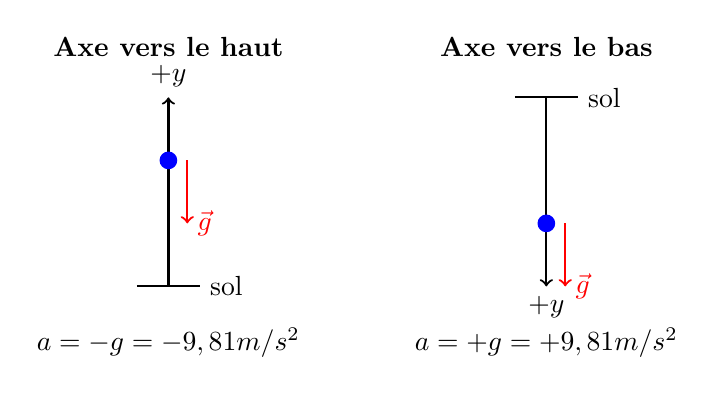
\begin{tikzpicture}[scale=0.8]
% Cas 1 : y vers le haut
\begin{scope}[shift={(0,0)}]
\draw[thick, ->] (0,0) -- (0,3) node[above] {$+y$};
\draw[thick] (-0.5,0) -- (0.5,0) node[right] {sol};
\fill[blue] (0,2) circle (4pt);
\draw[thick, red, ->] (0.3,2) -- (0.3,1) node[right] {$\vec{g}$};
\node[below] at (0,-0.5) {$a = -g = \SI{-9,81}{m/s^2}$};
\node[above] at (0,3.5) {\textbf{Axe vers le haut}};
\end{scope}
% Cas 2 : y vers le bas
\begin{scope}[shift={(6,0)}]
\draw[thick, ->] (0,3) -- (0,0) node[below] {$+y$};
\draw[thick] (-0.5,3) -- (0.5,3) node[right] {sol};
\fill[blue] (0,1) circle (4pt);
\draw[thick, red, ->] (0.3,1) -- (0.3,0) node[right] {$\vec{g}$};
\node[below] at (0,-0.5) {$a = +g = \SI{+9,81}{m/s^2}$};
\node[above] at (0,3.5) {\textbf{Axe vers le bas}};
\end{scope}
\end{tikzpicture}
\end{center}

\begin{attention}
La convention la plus courante (et celle utilisée dans ce cours) est de choisir l'axe $y$ \textbf{positif vers le haut}. Dans ce cas :
\[ a_y = -g = \SI{-9,81}{m/s^2} \]
Le signe négatif indique que l'accélération est dirigée vers le bas.
\end{attention}

\subsection{Équations de la chute libre}

Les équations de la chute libre sont les équations du MRUA appliquées à la direction verticale :

\begin{equationimportante}
\textbf{Équations de la chute libre} (axe $y$ positif vers le haut)
\begin{align}
v_y &= v_{iy} + a_y \Delta t = v_{iy} - g\Delta t \\[0.3cm]
\Delta y &= v_{iy} \Delta t + \frac{1}{2}a_y (\Delta t)^2 = v_{iy} \Delta t - \frac{1}{2}g(\Delta t)^2 \\[0.3cm]
v_y^2 &= v_{iy}^2 + 2a_y \Delta y = v_{iy}^2 - 2g\Delta y
\end{align}
\end{equationimportante}

\begin{remarque}[title=Notation]
\begin{itemize}
    \item $v_{iy}$ : vitesse initiale verticale (positive vers le haut, négative vers le bas)
    \item $v_y$ : vitesse finale verticale
    \item $\Delta y = y_f - y_i$ : déplacement vertical
    \item $g = \SI{9,81}{m/s^2}$ : valeur absolue de l'accélération gravitationnelle
\end{itemize}
\end{remarque}

\subsection{Cas particuliers}

\subsubsection{Objet lâché (sans vitesse initiale)}

\begin{exemple}{Outil tombant d'un mât (exemple maritime)}{}
Un matelot échappe une clé à molette du haut d'un mât situé à $\SI{25}{m}$ au-dessus du pont. 
\begin{enumerate}[label=\alph*)]
    \item Combien de temps met la clé pour atteindre le pont?
    \item À quelle vitesse frappe-t-elle le pont?
\end{enumerate}

\textbf{Données :}
\begin{itemize}
    \item $y_i = \SI{25}{m}$ (origine au pont, axe vers le haut)
    \item $y_f = \SI{0}{m}$
    \item $v_{iy} = \SI{0}{m/s}$ (lâchée, pas lancée)
    \item $a_y = \SI{-9,81}{m/s^2}$
\end{itemize}

\textbf{a) Temps de chute :}
\begin{align*}
\Delta y &= v_{iy} \Delta t - \frac{1}{2}g(\Delta t)^2 \\
0 - 25 &= 0 - \frac{1}{2}(9,81)(\Delta t)^2 \\
\Delta t &= \sqrt{\frac{2 \times 25}{9,81}} = \SI{2,26}{s}
\end{align*}

\textbf{b) Vitesse d'impact :}
\begin{align*}
v_y &= v_{iy} - g\Delta t \\
v_y &= 0 - 9,81 \times 2,26 = \SI{-22,2}{m/s}
\end{align*}

Le signe négatif indique que la vitesse est dirigée vers le bas. La clé frappe le pont à $\SI{22,2}{m/s}$ ($\SI{80}{km/h}$)!

\begin{attention}
C'est pourquoi le port du casque est obligatoire sur les chantiers navals et lors de certaines opérations à bord!
\end{attention}
\end{exemple}

\begin{pratiqueautonome}
Un conteneur se détache d'une grue portuaire et tombe d'une hauteur de $\SI{18}{m}$ au-dessus du quai.

\begin{enumerate}[label=\alph*)]
    \item Combien de temps dure la chute?
    \item À quelle vitesse le conteneur frappe-t-il le quai? Exprimez votre réponse en m/s et en km/h.
\end{enumerate}

\espaceresolution[6cm]
\reponsepratique{a) $\Delta t \approx \SI{1,9}{s}$ \quad b) $v \approx \SI{18,8}{m/s} \approx \SI{68}{km/h}$}
\end{pratiqueautonome}

\subsubsection{Objet lancé vers le haut}

\begin{exemple}{Fusée éclairante lancée à la main}{}
Un marin lance une fusée éclairante vers le haut avec une vitesse initiale de $\SI{15}{m/s}$ depuis le pont situé à $\SI{8}{m}$ au-dessus de l'eau.
\begin{enumerate}[label=\alph*)]
    \item Quelle hauteur maximale atteint-elle?
    \item Combien de temps reste-t-elle en l'air avant de toucher l'eau?
\end{enumerate}

\textbf{Données :}
\begin{itemize}
    \item $y_i = \SI{8}{m}$ (origine à la surface de l'eau)
    \item $v_{iy} = \SI{+15}{m/s}$ (vers le haut)
    \item $a_y = \SI{-9,81}{m/s^2}$
\end{itemize}

\textbf{a) Hauteur maximale :}

Au point le plus haut, la vitesse verticale est nulle ($v_y = 0$).
\begin{align*}
v_y^2 &= v_{iy}^2 - 2g\Delta y \\
0 &= 15^2 - 2(9,81)\Delta y \\
\Delta y &= \frac{225}{19,62} = \SI{11,5}{m}
\end{align*}

Hauteur maximale : $y_{max} = y_i + \Delta y = 8 + 11,5 = \SI{19,5}{m}$ au-dessus de l'eau.

\textbf{b) Temps total en l'air :}

La fusée touche l'eau quand $y_f = 0$.
\begin{align*}
y_f &= y_i + v_{iy} \Delta t - \frac{1}{2}g(\Delta t)^2 \\
0 &= 8 + 15\Delta t - 4,905(\Delta t)^2
\end{align*}

Équation quadratique : $4,905(\Delta t)^2 - 15\Delta t - 8 = 0$

\[ \Delta t = \frac{15 \pm \sqrt{225 + 4(4,905)(8)}}{2(4,905)} = \frac{15 \pm 18,5}{9,81} \]

Solution positive : $\Delta t = \SI{3,41}{s}$

La fusée reste en l'air pendant $\SI{3,41}{s}$.
\end{exemple}

\begin{pratiqueautonome}
Un marin lance verticalement une bouée de sauvetage lumineuse avec une vitesse initiale de $\SI{12}{m/s}$ depuis le pont situé à $\SI{6}{m}$ au-dessus de l'eau.

\begin{enumerate}[label=\alph*)]
    \item Quelle hauteur maximale atteint-elle au-dessus de l'eau?
    \item Combien de temps reste-t-elle en l'air avant de toucher l'eau?
\end{enumerate}

\textit{Indice : Pour a), au point le plus haut, $v_y = 0$. Pour b), résolvez $y_f = 0$.}

\espaceresolution[7cm]
\reponsepratique{a) $y_{max} \approx \SI{13,3}{m}$ \quad b) $\Delta t \approx \SI{2,8}{s}$}
\end{pratiqueautonome}

\begin{remarque}[title=Symétrie de la chute libre]
Pour un objet lancé vers le haut qui retombe au même niveau :
\begin{itemize}
    \item Le temps de montée égale le temps de descente
    \item La vitesse de retour a la même grandeur que la vitesse initiale (mais sens opposé)
\end{itemize}
Cette symétrie ne s'applique que si le point de départ et d'arrivée sont au même niveau.
\end{remarque}

\subsection{Application maritime : homme à la mer}

\begin{exemple}{Chute d'un homme à la mer}{}
Un marin tombe d'un pont situé à $\SI{12}{m}$ au-dessus de la surface de l'eau. En supposant qu'il ne saute pas (vitesse initiale nulle) :
\begin{enumerate}[label=\alph*)]
    \item Combien de temps dure la chute?
    \item À quelle vitesse entre-t-il dans l'eau?
\end{enumerate}

\textbf{a) Temps de chute :}
\[ \Delta t = \sqrt{\frac{2h}{g}} = \sqrt{\frac{2 \times 12}{9,81}} = \SI{1,56}{s} \]

\textbf{b) Vitesse d'entrée dans l'eau :}
\[ v = g \Delta t = 9,81 \times 1,56 = \SI{15,3}{m/s} \approx \SI{55}{km/h} \]

\begin{attention}
Une entrée dans l'eau à $\SI{55}{km/h}$ peut causer des blessures graves si la position du corps n'est pas adéquate. C'est pourquoi la formation à la survie en mer insiste sur la position à adopter lors d'une chute : bras croisés, jambes serrées, regard à l'horizon.
\end{attention}
\end{exemple}

\begin{center}
\renewcommand{\arraystretch}{1.5}
\begin{tabular}{|c|c|c|}
\hline
\rowcolor{bleuclair}
\textbf{Hauteur de chute} & \textbf{Temps de chute} & \textbf{Vitesse d'impact} \\
\hline
$\SI{5}{m}$ & $\SI{1,0}{s}$ & $\SI{10}{m/s}$ ($\SI{36}{km/h}$) \\
\hline
$\SI{10}{m}$ & $\SI{1,4}{s}$ & $\SI{14}{m/s}$ ($\SI{50}{km/h}$) \\
\hline
$\SI{15}{m}$ & $\SI{1,7}{s}$ & $\SI{17}{m/s}$ ($\SI{62}{km/h}$) \\
\hline
$\SI{20}{m}$ & $\SI{2,0}{s}$ & $\SI{20}{m/s}$ ($\SI{72}{km/h}$) \\
\hline
$\SI{30}{m}$ & $\SI{2,5}{s}$ & $\SI{24}{m/s}$ ($\SI{87}{km/h}$) \\
\hline
\end{tabular}
\end{center}

\begin{remarque}[title=L'universalité de la chute libre]
Les équations de la chute libre s'appliquent à tout objet : un conteneur qui tombe d'une grue, un plongeur qui saute d'un tremplin, une pomme qui tombe d'un arbre, ou une balle lancée en l'air. Seule la valeur de $g$ change selon la planète!

Sur la Lune : $g_{Lune} = \SI{1,62}{m/s^2}$ (environ 6 fois moins que sur Terre).
\end{remarque}

% =============================================================================
% CHAPITRE 1 - CINÉMATIQUE
% Partie 11 : Mouvement en deux dimensions
% Version maritime pour l'IMQ
% =============================================================================

% =============================================================================
\section{Mouvement en deux dimensions}
% =============================================================================

Jusqu'\`a pr\'esent, nous avons \'etudi\'e des mouvements en \textbf{une dimension} : des objets se d\'epla\c{c}ant le long d'une ligne droite (un axe $x$ ou $y$). Cependant, la plupart des mouvements r\'eels se produisent en \textbf{deux} ou \textbf{trois dimensions}.

\begin{remarque}[title=Exemples de mouvements en 2D]
\begin{itemize}
    \item Un navire qui navigue sur la mer (surface 2D)
    \item Une balle lanc\'ee qui suit une trajectoire courbe
    \item Un avion en vol (3D, mais on peut souvent simplifier en 2D)
    \item Un homme \`a la mer tomb\'e d'un navire en mouvement
\end{itemize}
\end{remarque}

\subsection{Le principe de d\'ecomposition}

La cl\'e pour analyser un mouvement en 2D est de le \textbf{d\'ecomposer} en deux mouvements ind\'ependants selon les axes $x$ et $y$.

\begin{definition}[title=Ind\'ependance des mouvements]
Dans un mouvement en deux dimensions, les composantes horizontale ($x$) et verticale ($y$) du mouvement sont \textbf{ind\'ependantes} l'une de l'autre.

Cela signifie que :
\begin{itemize}
    \item Le mouvement en $x$ n'affecte pas le mouvement en $y$
    \item Le mouvement en $y$ n'affecte pas le mouvement en $x$
    \item On peut analyser chaque direction s\'epar\'ement
\end{itemize}
\end{definition}

\begin{remarque}[title=Pourquoi peut-on d\'ecomposer? -- D\'evelopper l'intuition]
Cette ind\'ependance semble contre-intuitive! On pourrait penser qu'un objet lanc\'e horizontalement tombe \guillemotleft~moins vite~\guillemotright{} qu'un objet simplement l\^ach\'e. \textbf{C'est faux.}

\textbf{L'exp\'erience des deux balles :}

\begin{center}
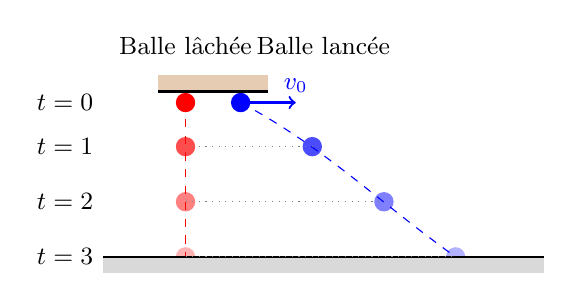
\begin{tikzpicture}[scale=0.7]
% Table
\fill[brown!40] (-1,3) rectangle (1,3.3);
\draw[thick] (-1,3) -- (1,3);
% Balle 1 (lâchée)
\fill[red] (-0.5,2.8) circle (5pt);
\fill[red!70] (-0.5,2) circle (5pt);
\fill[red!50] (-0.5,1) circle (5pt);
\fill[red!30] (-0.5,0) circle (5pt);
\draw[dashed, red] (-0.5,2.8) -- (-0.5,0);
\node[above] at (-0.5,3.5) {\small Balle l\^ach\'ee};
% Balle 2 (lancée)
\fill[blue] (0.5,2.8) circle (5pt);
\fill[blue!70] (1.8,2) circle (5pt);
\fill[blue!50] (3.1,1) circle (5pt);
\fill[blue!30] (4.4,0) circle (5pt);
\draw[dashed, blue] (0.5,2.8) .. controls (2,2) and (3,1) .. (4.4,0);
\draw[thick, blue, ->] (0.5,2.8) -- (1.5,2.8) node[above] {\small $v_0$};
\node[above] at (2,3.5) {\small Balle lanc\'ee};
% Sol
\fill[gray!30] (-2,-0.3) rectangle (6,0);
\draw[thick] (-2,0) -- (6,0);
% Temps
\node[left] at (-2,2.8) {\small $t=0$};
\node[left] at (-2,2) {\small $t=1$};
\node[left] at (-2,1) {\small $t=2$};
\node[left] at (-2,0) {\small $t=3$};
% Lignes horizontales pour montrer la simultanéité
\draw[dotted, gray] (-0.5,2) -- (1.8,2);
\draw[dotted, gray] (-0.5,1) -- (3.1,1);
\draw[dotted, gray] (-0.5,0) -- (4.4,0);
\end{tikzpicture}
\end{center}

Deux balles sont \`a la m\^eme hauteur. Au m\^eme instant, l'une est \textbf{l\^ach\'ee} et l'autre est \textbf{lanc\'ee horizontalement}. R\'esultat : \textbf{elles touchent le sol en m\^eme temps!}

La vitesse horizontale de la balle lanc\'ee n'affecte pas sa chute. Les deux balles subissent exactement la m\^eme acc\'el\'eration verticale ($g$), donc elles tombent \`a la m\^eme vitesse verticale.

\textbf{Analogie maritime :} Imaginez un matelot au sommet d'un m\^at sur un navire avanc ant \`a vitesse constante. S'il l\^ache une cl\'e :
\begin{itemize}
    \item \textbf{Du point de vue du matelot} : la cl\'e tombe droit vers le bas
    \item \textbf{Du point de vue du quai} : la cl\'e suit une trajectoire courbe (parabole)
\end{itemize}
La cl\'e \guillemotleft~conserve~\guillemotright{} la vitesse horizontale du navire pendant toute sa chute, mais cette vitesse horizontale n'affecte en rien la dur\'ee de la chute!

\textbf{Essayez en classe :} Placez deux pi\`eces de monnaie sur le bord d'une table. Frappez-en une horizontalement avec une r\`egle pendant que l'autre tombe. \'Ecoutez : un seul \guillemotleft~clic~\guillemotright{} au sol!
\end{remarque}

\begin{attention}[title=Principe fondamental]
\textbf{Pour r\'esoudre un probl\`eme de mouvement en 2D :}
\begin{enumerate}
    \item D\'ecomposer le mouvement en composantes $x$ et $y$
    \item R\'esoudre \textbf{s\'epar\'ement} le mouvement en $x$ et en $y$
    \item Relier les deux par le \textbf{temps} $\Delta t$ (qui est le m\^eme pour les deux)
    \item Recombiner les r\'esultats si n\'ecessaire
\end{enumerate}
\end{attention}

\subsection{D\'ecomposition d'un vecteur}

Tout vecteur (position, vitesse, acc\'el\'eration) peut \^etre d\'ecompos\'e en composantes :

\begin{center}
\begin{tikzpicture}[scale=1.3]
% Axes
\draw[axe, thick, ->] (0,0) -- (4,0) node[right] {$x$};
\draw[axe, thick, ->] (0,0) -- (0,3) node[above] {$y$};
% Vecteur
\draw[very thick, red, ->] (0,0) -- (3,2) node[above right] {$\vec{v}$};
% Composantes
\draw[thick, blue, ->] (0,0) -- (3,0) node[below] {$v_x$};
\draw[thick, green!60!black, ->] (3,0) -- (3,2) node[right] {$v_y$};
% Angle
\draw[thick] (0.7,0) arc (0:33.7:0.7);
\node at (1,0.3) {$\theta$};
% Rectangle pointillé
\draw[dashed, gray] (0,2) -- (3,2);
\draw[dashed, gray] (0,0) -- (0,2);
\end{tikzpicture}
\end{center}

\begin{equationimportante}
\textbf{D\'ecomposition d'un vecteur}
\begin{align}
v_x &= v \cos\theta \\
v_y &= v \sin\theta
\end{align}
o\`u $\theta$ est l'angle par rapport \`a l'horizontale.

\textbf{Recomposition (module et direction)}
\begin{align}
v &= \sqrt{v_x^2 + v_y^2} \\
\theta &= \arctan\left(\frac{v_y}{v_x}\right)
\end{align}
\end{equationimportante}

\subsection{Exemple : navigation d'un navire}

\begin{exemple}{Cap et vitesse d'un navire}{}
Un navire navigue \`a $\SI{15}{n\oe{}uds}$ avec un cap de $30°$ par rapport \`a l'est (c'est-\`a-dire $30°$ nord de l'est).

Quelles sont les composantes est-ouest et nord-sud de sa vitesse?

\begin{center}
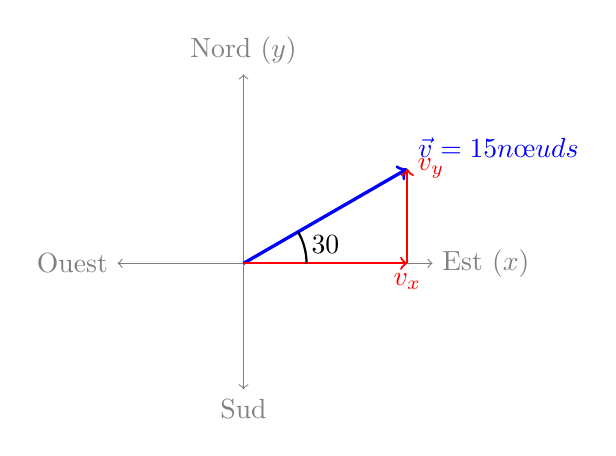
\begin{tikzpicture}[scale=0.8]
% Rose des vents simplifiée
\draw[gray, ->] (0,0) -- (3,0) node[right] {Est ($x$)};
\draw[gray, ->] (0,0) -- (0,3) node[above] {Nord ($y$)};
\draw[gray, ->] (0,0) -- (-2,0) node[left] {Ouest};
\draw[gray, ->] (0,0) -- (0,-2) node[below] {Sud};
% Vecteur vitesse
\draw[very thick, blue, ->] (0,0) -- (2.6,1.5) node[above right] {$\vec{v} = \SI{15}{n\oe{}uds}$};
% Composantes
\draw[thick, red, ->] (0,0) -- (2.6,0) node[below] {$v_x$};
\draw[thick, red, ->] (2.6,0) -- (2.6,1.5) node[right] {$v_y$};
% Angle
\draw[thick] (1,0) arc (0:30:1);
\node at (1.3,0.3) {$30°$};
% Navire
\node at (1.3,0.75) {\small $\blacktriangle$};
\end{tikzpicture}
\end{center}

\textbf{Composante est-ouest :}
\[ v_x = v \cos\theta = 15 \cos 30° = 15 \times 0,866 = \SI{13,0}{n\oe{}uds} \]

\textbf{Composante nord-sud :}
\[ v_y = v \sin\theta = 15 \sin 30° = 15 \times 0,5 = \SI{7,5}{n\oe{}uds} \]

Le navire se d\'eplace donc \`a $\SI{13,0}{n\oe{}uds}$ vers l'est et $\SI{7,5}{n\oe{}uds}$ vers le nord.
\end{exemple}

\subsection{Application au projectile}

Le mouvement d'un \textbf{projectile} (objet lanc\'e dans l'air) est l'exemple classique de mouvement en 2D. On le d\'ecompose en :

\begin{center}
\renewcommand{\arraystretch}{1.5}
\begin{tabular}{|c|c|}
\hline
\rowcolor{bleuclair}
\textbf{Direction horizontale ($x$)} & \textbf{Direction verticale ($y$)} \\
\hline
Aucune force horizontale & Gravit\'e (vers le bas) \\
\hline
$a_x = 0$ & $a_y = -g$ \\
\hline
\textbf{MRU} (vitesse constante) & \textbf{Chute libre} (MRUA) \\
\hline
\end{tabular}
\end{center}

\begin{remarque}[title=Ce qui relie les deux directions]
Les mouvements en $x$ et en $y$ sont ind\'ependants, mais ils partagent le m\^eme \textbf{temps} $\Delta t$.

C'est cette variable commune qui permet de relier les deux directions et de d\'eterminer, par exemple, o\`u un projectile atterrit.
\end{remarque}

Dans la section suivante, nous appliquerons ces principes \`a l'\'etude compl\`ete du mouvement d'un projectile.

% =============================================================================
% CHAPITRE 1 - CINÉMATIQUE
% Partie 9 : Mouvement d'un projectile
% Version maritime pour l'IMQ
% =============================================================================

% =============================================================================
\section{Mouvement d'un projectile}
% =============================================================================
\subsection*{Un peu d'histoire : Galilée et la décomposition du mouvement}

Avant \textbf{Galilée} (1564--1642), les savants croyaient qu'un boulet de canon suivait d'abord une ligne droite, puis tombait verticalement une fois sa « force » épuisée. Cette vision, héritée d'Aristote, ne correspondait pas aux observations.

La contribution révolutionnaire de Galilée fut de comprendre que \textbf{le mouvement horizontal et le mouvement vertical sont indépendants}. Un objet lancé continue d'avancer horizontalement \emph{en même temps} qu'il tombe verticalement --- les deux mouvements se superposent sans s'influencer mutuellement.

\begin{remarque}[title=Le principe d'indépendance des mouvements]
Galilée démontra ce principe par une expérience de pensée : une bille lâchée du haut du mât d'un navire en mouvement tombe au pied du mât, pas derrière. La bille conserve le mouvement horizontal du navire pendant sa chute.

Ce principe est fondamental pour les navigateurs : un objet qui tombe d'un navire en mouvement ne tombe pas « en arrière » --- il conserve la vitesse du navire.
\end{remarque}

Cette décomposition en mouvements indépendants est la clé pour analyser les projectiles : on traite séparément la direction horizontale (mouvement uniforme) et la direction verticale (chute libre), puis on combine les résultats.

\vspace{0.5cm}

Un \textbf{projectile} est un objet lanc\'e dans l'air qui se d\'eplace ensuite uniquement sous l'influence de la gravit\'e. C'est l'application directe des principes du mouvement en 2D que nous venons de voir.

\begin{remarque}[title=Questions types que nous allons r\'esoudre]
Dans cette section, vous apprendrez \`a r\'epondre aux questions suivantes :
\begin{itemize}
    \item Quelle est la \textbf{port\'ee} (distance horizontale) d'un projectile?
    \item Quelle \textbf{hauteur maximale} atteint-il?
    \item Combien de \textbf{temps} reste-t-il en l'air?
    \item O\`u \textbf{atterrit} un objet lanc\'e horizontalement?
    \item \`A quel angle faut-il lancer pour atteindre une cible?
    \item O\`u tombe un objet l\^ach\'e d'un navire en mouvement?
\end{itemize}
\end{remarque}

\begin{definition}[title=Projectile]
Un projectile est un corps lanc\'e avec une vitesse initiale quelconque et qui se d\'eplace sous la seule action de la gravit\'e (r\'esistance de l'air n\'eglig\'ee).

Exemples : ballon lanc\'e, balle de baseball, fus\'ee \'eclairante, lance-amarre, boulet de canon.
\end{definition}

\begin{attention}[title=Rappel fondamental]
Puisque la gravit\'e est la \textbf{seule force} et qu'elle agit \textbf{verticalement} :
\begin{itemize}
    \item En $x$ : pas d'acc\'el\'eration ($a_x = 0$) $\Rightarrow$ \textbf{MRU}
    \item En $y$ : acc\'el\'eration constante ($a_y = -g$) $\Rightarrow$ \textbf{Chute libre}
\end{itemize}
La composante horizontale de la vitesse \textbf{reste constante} tout au long du vol!
\end{attention}

\subsection{Strat\'egie de r\'esolution}

\begin{remarque}[title=Strat\'egie de r\'esolution -- TR\`ES IMPORTANT]
Pour r\'esoudre des probl\`emes de projectile en 2D, il faut \textbf{toujours} :
\begin{enumerate}
    \item \textbf{D\'ecomposer} le mouvement en deux directions : $x$ (horizontal) et $y$ (vertical)
    \item \textbf{Traiter s\'epar\'ement} chaque direction
    \item \textbf{Relier} les deux directions par le \textbf{temps} $\Delta t$ (qui est le m\^eme pour les deux)
\end{enumerate}
\end{remarque}

\begin{center}
\begin{tikzpicture}[scale=0.9]
% Axes
\draw[axe, thick, ->] (0,0) -- (8,0) node[right] {$x$};
\draw[axe, thick, ->] (0,0) -- (0,5) node[above] {$y$};
% Trajectoire
\draw[very thick, blue, domain=0:7, samples=50] plot (\x, {3*\x/7 + 0.5 - 0.12*\x*\x});
% Positions
\foreach \t in {0,1,2,3,4,5,6,7} {
    \pgfmathsetmacro{\ypos}{3*\t/7 + 0.5 - 0.12*\t*\t}
    \fill[blue] (\t, \ypos) circle (3pt);
}
% Vecteurs vitesse
\draw[thick, red, ->] (0,0.5) -- (1,0.93) node[above right] {\small $\vec{v}_0$};
\draw[thick, red, ->] (3.5,2.03) -- (4.5,1.89);
\draw[thick, red, ->] (7,0.5) -- (8,-0.36);
% Composantes à t=0
\draw[thick, green!60!black, ->] (0,0.5) -- (1,0.5) node[below] {\small $v_{0x}$};
\draw[thick, orange, ->] (0,0.5) -- (0,0.93) node[left] {\small $v_{0y}$};
% Annotations
\node at (3.5,4) {\textbf{Trajectoire parabolique}};
\node[blue] at (3.5,-0.5) {En $x$ : MRU ($v_x$ constante)};
\node[blue] at (3.5,-1) {En $y$ : Chute libre ($a_y = -g$)};
\end{tikzpicture}
\end{center}

\subsection{Décomposition de la vitesse initiale}

Si le projectile est lancé avec une vitesse initiale $v_0$ faisant un angle $\theta$ avec l'horizontale :

\begin{equationimportante}
\textbf{Composantes de la vitesse initiale}
\begin{align}
v_{0x} &= v_0 \cos\theta \\[0.2cm]
v_{0y} &= v_0 \sin\theta
\end{align}
\end{equationimportante}

\begin{center}
\begin{tikzpicture}[scale=1.2]
% Axes
\draw[axe, thick, ->] (0,0) -- (4,0) node[right] {$x$};
\draw[axe, thick, ->] (0,0) -- (0,3) node[above] {$y$};
% Vecteur v0
\draw[very thick, red, ->] (0,0) -- (3,2) node[above right] {$\vec{v}_0$};
% Composantes
\draw[thick, green!60!black, ->] (0,0) -- (3,0) node[below] {$v_{0x} = v_0 \cos\theta$};
\draw[thick, orange, ->] (3,0) -- (3,2) node[right] {$v_{0y} = v_0 \sin\theta$};
% Angle
\draw[thick] (0.8,0) arc (0:33.7:0.8) node[midway, right] {$\theta$};
% Valeur de v0
\node at (1.2,1.3) {$v_0$};
\end{tikzpicture}
\end{center}

\subsection{Équations du mouvement}

\begin{center}
\renewcommand{\arraystretch}{1.8}
\begin{tabular}{|c|c|}
\hline
\rowcolor{bleuclair}
\textbf{Direction horizontale ($x$)} & \textbf{Direction verticale ($y$)} \\
\hline
MRU (vitesse constante) & Chute libre (MRUA) \\
\hline
$a_x = 0$ & $a_y = -g$ \\
\hline
$v_x = v_{0x} = v_0 \cos\theta$ & $v_y = v_{0y} - g\Delta t = v_0 \sin\theta - g\Delta t$ \\
\hline
$\Delta x = v_{0x} \Delta t = (v_0 \cos\theta) \Delta t$ & $\Delta y = v_{0y} \Delta t - \dfrac{1}{2}g(\Delta t)^2$ \\
\hline
& $v_y^2 = v_{0y}^2 - 2g\Delta y$ \\
\hline
\end{tabular}
\end{center}

\begin{remarque}[title=Le temps relie les deux directions]
Le temps $\Delta t$ est \textbf{le même} pour le mouvement horizontal et vertical. C'est ce qui permet de relier les deux directions et de résoudre les problèmes.
\end{remarque}

\subsection{Caract\'eristiques de la trajectoire}

Lors de l'analyse d'un projectile, on s'int\'eresse souvent \`a trois grandeurs cl\'es. Plut\^ot que de m\'emoriser des formules sp\'ecifiques, il est pr\'ef\'erable de comprendre \textbf{comment les trouver} \`a partir des \'equations de base.

\begin{center}
\begin{tikzpicture}[scale=0.9]
% Axes
\draw[axe, thick, ->] (0,0) -- (9,0) node[right] {$x$};
\draw[axe, thick, ->] (0,0) -- (0,5) node[above] {$y$};

% Trajectoire parabolique (portée = 7, h_max = 3.5)
\draw[very thick, blue, domain=0:7, samples=100] plot (\x, {2*\x - 2*\x*\x/7});

% Point de départ
\fill[red] (0,0) circle (4pt);
\node[below left] at (0,0) {D\'epart};

% Point d'arrivée
\fill[red] (7,0) circle (4pt);
\node[below right] at (7,0) {Arriv\'ee};

% Point au sommet (à x = 3.5, y = 3.5)
\fill[green!60!black] (3.5,3.5) circle (4pt);
\node[above] at (3.5,3.8) {Sommet};

% Hauteur maximale
\draw[<->, thick, green!60!black] (3.5,0) -- (3.5,3.5);
\node[right, green!60!black] at (3.6,1.75) {$h_{max}$};
\draw[dashed, gray] (0,3.5) -- (3.5,3.5);

% Portée
\draw[<->, thick, orange] (0,-0.7) -- (7,-0.7);
\node[below, orange] at (3.5,-0.7) {Port\'ee};

% Vecteur vitesse initiale
\draw[very thick, red, ->] (0,0) -- (1.2,1.5) node[above left] {$\vec{v}_0$};
\draw[thick] (0.5,0) arc (0:51:0.5);
\node at (0.85,0.35) {$\theta$};

% Vecteur vitesse au sommet (horizontal)
\draw[very thick, red, ->] (3.5,3.5) -- (4.7,3.5) node[above] {$\vec{v}$};
\node[below] at (4.5,3.2) {\small ($v_y = 0$)};

% Vecteur vitesse finale
\draw[very thick, red, ->] (7,0) -- (8.2,-1.5);

% Temps de montée et descente
\draw[<->, thick, purple] (0,4.3) -- (3.5,4.3);
\node[above, purple] at (1.75,4.3) {\small $t_{mont\acute{e}e}$};
\draw[<->, thick, purple] (3.5,4.3) -- (7,4.3);
\node[above, purple] at (5.25,4.3) {\small $t_{descente}$};

% Annotation temps total
\node[below] at (3.5,-1.4) {Temps de vol total : $\Delta t = t_{mont\acute{e}e} + t_{descente}$};

\end{tikzpicture}
\end{center}

\begin{remarque}[title=Observations importantes sur le sch\'ema]
\begin{itemize}
    \item Au \textbf{sommet}, la vitesse n'est \textbf{pas nulle}! Seule la composante verticale $v_y$ est nulle. La composante horizontale $v_x$ reste constante tout au long du vol.
    \item Pour un projectile lanc\'e et retombant au m\^eme niveau, le temps de mont\'ee \'egale le temps de descente (sym\'etrie).
    \item La trajectoire est une \textbf{parabole}, cons\'equence directe du MRU en $x$ et du MRUA en $y$.
\end{itemize}
\end{remarque}

\subsubsection{Port\'ee horizontale}

\begin{definition}[title=Port\'ee]
La \textbf{port\'ee} est la distance horizontale totale parcourue par le projectile entre son lancement et son atterrissage.
\end{definition}

\textbf{Comment la trouver :}
\begin{enumerate}
    \item D\'eterminer le \textbf{temps de vol} $\Delta t$ en utilisant l'\'equation verticale (quand $y$ revient au niveau d'arriv\'ee)
    \item Utiliser ce temps dans l'\'equation horizontale : $\text{Port\'ee} = v_{0x} \cdot \Delta t$
\end{enumerate}

\begin{remarque}
Pour un projectile lanc\'e et retombant au m\^eme niveau, la port\'ee est maximale lorsque l'angle de lancement est de $45^\circ$.
\end{remarque}

\subsubsection{Hauteur maximale}

\begin{definition}[title=Hauteur maximale]
La \textbf{hauteur maximale} est l'altitude la plus \'elev\'ee atteinte par le projectile au cours de son vol.
\end{definition}

\textbf{Comment la trouver :}

Au point le plus haut, la composante verticale de la vitesse s'annule ($v_y = 0$). On utilise alors l'\'equation $v_y^2 = v_{0y}^2 - 2g\Delta y$ avec $v_y = 0$ pour trouver $\Delta y_{max}$.

\subsubsection{Temps de vol}

\begin{definition}[title=Temps de vol]
Le \textbf{temps de vol} est la dur\'ee totale pendant laquelle le projectile reste en l'air, du lancement jusqu'\`a l'atterrissage.
\end{definition}

\textbf{Comment le trouver :}

On utilise l'\'equation de position verticale $\Delta y = v_{0y} \Delta t - \frac{1}{2}g(\Delta t)^2$ en fixant $\Delta y$ \'egal au d\'eplacement vertical total (souvent z\'ero si retour au m\^eme niveau, ou n\'egatif si atterrissage plus bas).

\begin{attention}[title=Approche recommand\'ee]
Plut\^ot que de m\'emoriser des formules sp\'ecifiques pour la port\'ee, la hauteur maximale ou le temps de vol, il est beaucoup plus efficace de :
\begin{enumerate}
    \item Ma\^itriser les \'equations de base (MRU en $x$, chute libre en $y$)
    \item Identifier ce qu'on cherche et ce qu'on conna\^it
    \item Appliquer la strat\'egie de d\'ecomposition syst\'ematiquement
\end{enumerate}
Cette approche fonctionne pour \textbf{tous} les probl\`emes de projectile, m\^eme les plus complexes!
\end{attention}

\subsection{Exemples}

\begin{exemple}{Ballon de soccer (exemple terrestre)}{ballon-soccer}
Un joueur botte un ballon avec une vitesse initiale de $\SI{20}{m/s}$ \`a un angle de $30^\circ$ par rapport au sol.
\begin{enumerate}[label=\alph*)]
    \item Quelle est la port\'ee du tir?
    \item Quelle hauteur maximale atteint le ballon?
    \item Combien de temps le ballon reste-t-il en l'air?
\end{enumerate}

\textbf{Donn\'ees :}
\begin{itemize}
    \item $v_0 = \SI{20}{m/s}$, $\theta = 30^\circ$
    \item $v_{0x} = 20 \cos 30^\circ = \SI{17,3}{m/s}$
    \item $v_{0y} = 20 \sin 30^\circ = \SI{10}{m/s}$
\end{itemize}

\textbf{b) Hauteur maximale :} (on commence par celle-ci car elle ne n\'ecessite pas le temps)

Au point le plus haut, $v_y = 0$. Utilisons $v_y^2 = v_{0y}^2 - 2g\Delta y$ :
\begin{align*}
0 &= 10^2 - 2(9,81)\Delta y_{max} \\
\Delta y_{max} &= \frac{100}{19,62} = \SI{5,10}{m}
\end{align*}

\textbf{c) Temps de vol :}

Le ballon revient au sol quand $\Delta y = 0$. Utilisons $\Delta y = v_{0y} \Delta t - \frac{1}{2}g(\Delta t)^2$ :
\begin{align*}
0 &= 10 \Delta t - 4,905(\Delta t)^2 \\
0 &= \Delta t (10 - 4,905 \Delta t)
\end{align*}

Solutions : $\Delta t = 0$ (d\'epart) ou $\Delta t = \frac{10}{4,905} = \SI{2,04}{s}$ (atterrissage)

\textbf{a) Port\'ee :}

Maintenant qu'on conna\^it le temps de vol :
\[ \text{Port\'ee} = v_{0x} \cdot \Delta t = 17,3 \times 2,04 = \SI{35,3}{m} \]
\end{exemple}

\begin{exemple}{Lance-amarre (exemple maritime)}{lance-amarre}
Un marin utilise un lance-amarre pour envoyer une ligne vers un quai. L'appareil lance le projectile à $\SI{25}{m/s}$ avec un angle de $40^\circ$. Le marin se trouve sur le pont à $\SI{6}{m}$ au-dessus du niveau du quai.

Quelle est la portée horizontale du tir?

\textbf{Données :}
\begin{itemize}
    \item $v_0 = \SI{25}{m/s}$, $\theta = 40^\circ$
    \item $y_i = \SI{6}{m}$, $y_f = \SI{0}{m}$ (niveau du quai)
    \item $v_{0x} = 25 \cos 40^\circ = \SI{19,2}{m/s}$
    \item $v_{0y} = 25 \sin 40^\circ = \SI{16,1}{m/s}$
\end{itemize}

\textbf{Étape 1 : Trouver le temps de vol}

On utilise l'équation en $y$ :
\begin{align*}
y_f &= y_i + v_{0y} \Delta t - \frac{1}{2}g(\Delta t)^2 \\
0 &= 6 + 16,1 \Delta t - 4,905(\Delta t)^2
\end{align*}

Équation quadratique : $4,905(\Delta t)^2 - 16,1\Delta t - 6 = 0$

\[ \Delta t = \frac{16,1 + \sqrt{259,2 + 117,7}}{9,81} = \frac{16,1 + 19,4}{9,81} = \SI{3,62}{s} \]

\textbf{Étape 2 : Calculer la portée}
\[ \Delta x = v_{0x} \Delta t = 19,2 \times 3,62 = \SI{69,5}{m} \]

Le lance-amarre peut atteindre une cible à environ $\SI{70}{m}$.

\begin{remarque}
Le fait de lancer depuis une position surélevée augmente significativement la portée par rapport à un lancer au niveau du sol.
\end{remarque}
\end{exemple}

\begin{pratiqueautonome}
Un lance-amarre tire une ligne avec une vitesse initiale de $\SI{30}{m/s}$ à un angle de $40^\circ$ au-dessus de l'horizontale, depuis une hauteur de $\SI{4}{m}$ au-dessus de l'eau.

\begin{enumerate}[label=\alph*)]
    \item Décomposez la vitesse initiale en ses composantes $v_{0x}$ et $v_{0y}$.
    \item Calculez la portée horizontale (distance où la ligne touche l'eau).
\end{enumerate}

\textit{Indice : Trouvez d'abord le temps de vol en résolvant $y_f = 0$.}

\espaceresolution[8cm]
\reponsepratique{a) $v_{0x} \approx \SI{23,0}{m/s}$, $v_{0y} \approx \SI{19,3}{m/s}$ \quad b) Portée $\approx \SI{97}{m}$}
\end{pratiqueautonome}

\begin{exemple}{Homme à la mer depuis un navire en mouvement}{homme-a-la-mer}
Un marin tombe d'un navire qui avance à $\SI{8}{n\oe{}uds}$. Il tombe d'une hauteur de $\SI{10}{m}$. À quelle distance horizontale du point de chute le marin entre-t-il dans l'eau?

\textbf{Analyse :} Au moment de la chute, le marin a la même vitesse horizontale que le navire. C'est un projectile lancé horizontalement ($\theta = 0^\circ$).

\textbf{Conversion de la vitesse :}
\[ v_{0x} = \SI{8}{n\oe{}uds} \times \frac{\SI{0,5144}{m/s}}{\SI{1}{n\oe{}ud}} = \SI{4,1}{m/s} \]

\textbf{Données :}
\begin{itemize}
    \item $v_{0x} = \SI{4,1}{m/s}$ (vitesse du navire)
    \item $v_{0y} = \SI{0}{m/s}$ (chute, pas saut)
    \item $\Delta y = \SI{-10}{m}$
\end{itemize}

\textbf{Temps de chute :} On utilise l'équation de position verticale avec $v_{0y} = 0$ :
\begin{align*}
\Delta y &= v_{0y} \Delta t - \frac{1}{2}g(\Delta t)^2 \\
-10 &= 0 - \frac{1}{2}(9,81)(\Delta t)^2 \\
(\Delta t)^2 &= \frac{2 \times 10}{9,81} = 2,04 \\
\Delta t &= \SI{1,43}{s}
\end{align*}

\textbf{Distance horizontale :}
\[ \Delta x = v_{0x} \Delta t = 4,1 \times 1,43 = \SI{5,9}{m} \]

Le marin entre dans l'eau à environ $\SI{6}{m}$ en avant du point d'où il est tombé (par rapport à l'eau, pas par rapport au navire qui continue d'avancer).

\begin{attention}
Pendant ce temps, le navire a aussi avancé de $\SI{5,9}{m}$. Du point de vue d'un observateur sur le navire, le marin semble tomber verticalement! C'est le principe de l'indépendance des mouvements.
\end{attention}
\end{exemple}

\begin{exemple}{Probl\`eme inverse : trouver l'angle de lancement}{probleme-inverse-angle}
Un canon lance-amarre doit atteindre un quai situ\'e \`a $\SI{50}{m}$ de distance horizontale. La vitesse de sortie du projectile est de $\SI{30}{m/s}$. Le canon et le quai sont au m\^eme niveau.

\`A quel angle faut-il r\'egler le canon?

\textbf{Donn\'ees :}
\begin{itemize}
    \item Port\'ee souhait\'ee : $\Delta x = \SI{50}{m}$
    \item Vitesse initiale : $v_0 = \SI{30}{m/s}$
    \item D\'eplacement vertical : $\Delta y = 0$ (m\^eme niveau)
    \item Inconnue : $\theta = ?$
\end{itemize}

\textbf{Strat\'egie :} On doit relier la port\'ee \`a l'angle. Exprimons $\Delta x$ en fonction de $\theta$.

\textbf{\'Etape 1 : Trouver le temps de vol en fonction de $\theta$}

Quand le projectile revient au m\^eme niveau, $\Delta y = 0$ :
\begin{align*}
\Delta y &= v_{0y} \Delta t - \frac{1}{2}g(\Delta t)^2 \\
0 &= (v_0 \sin\theta) \Delta t - \frac{1}{2}g(\Delta t)^2 \\
0 &= \Delta t \left( v_0 \sin\theta - \frac{1}{2}g \Delta t \right)
\end{align*}

Solutions : $\Delta t = 0$ (d\'epart) ou $\Delta t = \dfrac{2 v_0 \sin\theta}{g}$ (atterrissage)

\textbf{\'Etape 2 : Exprimer la port\'ee}
\begin{align*}
\Delta x &= v_{0x} \cdot \Delta t = (v_0 \cos\theta) \cdot \frac{2 v_0 \sin\theta}{g} \\
\Delta x &= \frac{2 v_0^2 \sin\theta \cos\theta}{g} = \frac{v_0^2 \sin(2\theta)}{g}
\end{align*}

(On utilise l'identit\'e trigonom\'etrique $2\sin\theta\cos\theta = \sin(2\theta)$)

\textbf{\'Etape 3 : Isoler $\theta$}
\begin{align*}
\sin(2\theta) &= \frac{g \cdot \Delta x}{v_0^2} = \frac{9,81 \times 50}{30^2} = \frac{490,5}{900} = 0,545
\end{align*}

\[ 2\theta = \arcsin(0,545) = 33,0^\circ \quad \Rightarrow \quad \theta = 16,5^\circ \]

\textbf{Attention!} L'\'equation $\sin(2\theta) = 0,545$ a \textbf{deux solutions} entre $0^\circ$ et $90^\circ$ :
\begin{itemize}
    \item $2\theta = 33,0^\circ$ $\Rightarrow$ $\theta_1 = 16,5^\circ$ (tir tendu)
    \item $2\theta = 180^\circ - 33,0^\circ = 147^\circ$ $\Rightarrow$ $\theta_2 = 73,5^\circ$ (tir en cloche)
\end{itemize}

\begin{center}
\begin{tikzpicture}[scale=0.55]
% Axes
\draw[axe, thick, ->] (0,0) -- (8,0) node[right] {$x$};
\draw[axe, thick, ->] (0,0) -- (0,5) node[above] {$y$};

% Trajectoire basse (16.5$^\circ$)
\draw[very thick, blue, domain=0:7, samples=50] plot (\x, {0.42*\x - 0.03*\x*\x});
\draw[thick, blue, ->] (0,0) -- (1.4,0.42) node[above left] {\small $\theta_1 = 16,5^\circ$};

% Trajectoire haute (73.5$^\circ$)
\draw[very thick, red, domain=0:7, samples=50] plot (\x, {2.38*\x - 0.17*\x*\x});
\draw[thick, red, ->] (0,0) -- (0.42,1.4) node[above left] {\small $\theta_2 = 73,5^\circ$};

% Point cible
\fill[green!60!black] (7,0) circle (5pt);
\node[below] at (7,0) {Cible};

% Légende
\node[blue] at (5,0.8) {\small Tir tendu};
\node[red] at (2,4) {\small Tir en cloche};
\end{tikzpicture}
\end{center}

\textbf{R\'eponse :} Deux angles sont possibles : $\theta_1 = 16,5^\circ$ ou $\theta_2 = 73,5^\circ$.

\begin{remarque}[title=Choix pratique]
En pratique, le tir tendu ($16,5^\circ$) est souvent pr\'ef\'er\'e car :
\begin{itemize}
    \item Le temps de vol est plus court (la ligne reste tendue)
    \item Le tir est moins affect\'e par le vent
    \item La pr\'ecision est g\'en\'eralement meilleure
\end{itemize}
Le tir en cloche peut \^etre utile pour passer par-dessus un obstacle.
\end{remarque}
\end{exemple}

\begin{exemple}{Port\'ee maximale impossible}{portee-maximale-impossible}
Avec le m\^eme canon ($v_0 = \SI{30}{m/s}$), peut-on atteindre une cible \`a $\SI{100}{m}$?

\textbf{V\'erification :}
\[ \sin(2\theta) = \frac{g \cdot \Delta x}{v_0^2} = \frac{9,81 \times 100}{900} = 1,09 \]

Puisque $\sin(2\theta)$ ne peut jamais d\'epasser 1, \textbf{aucun angle} ne permet d'atteindre cette cible!

\textbf{Port\'ee maximale :} Elle est atteinte quand $\sin(2\theta) = 1$, soit $\theta = 45^\circ$ :
\[ \Delta x_{max} = \frac{v_0^2}{g} = \frac{900}{9,81} = \SI{91,7}{m} \]

La cible \`a $\SI{100}{m}$ est hors de port\'ee.
\end{exemple}

\subsection{Projectile lanc\'e horizontalement}

Un cas particulier important est le projectile lancé \textbf{horizontalement} (angle $\theta = 0^\circ$).

\begin{center}
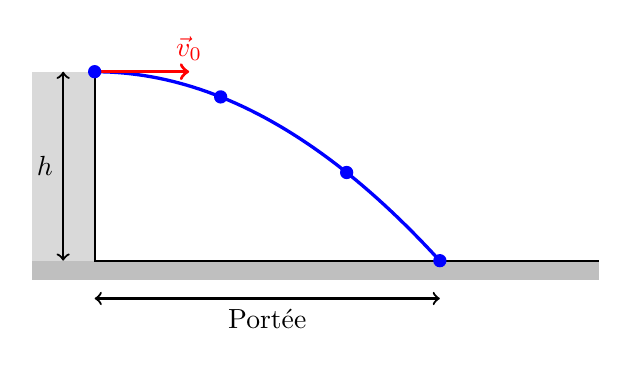
\begin{tikzpicture}[scale=0.8]
% Falaise
\fill[gray!30] (-1,3) rectangle (0,0);
\fill[gray!50] (-1,0) rectangle (8,-0.3);
\draw[thick] (0,3) -- (0,0) -- (8,0);
% Trajectoire
\draw[very thick, blue, domain=0:5.5, samples=50] plot (\x, {3 - 0.1*\x*\x});
% Vecteur vitesse initiale
\draw[very thick, red, ->] (0,3) -- (1.5,3) node[above] {$\vec{v}_0$};
% Points et vecteurs
\fill[blue] (0,3) circle (3pt);
\fill[blue] (2,2.6) circle (3pt);
\fill[blue] (4,1.4) circle (3pt);
\fill[blue] (5.48,0) circle (3pt);
% Hauteur
\draw[<->, thick] (-0.5,0) -- (-0.5,3) node[midway, left] {$h$};
% Portée
\draw[<->, thick] (0,-0.6) -- (5.48,-0.6) node[midway, below] {Portée};
\end{tikzpicture}
\end{center}

Dans ce cas :
\begin{itemize}
    \item $v_{0x} = v_0$ (toute la vitesse est horizontale)
    \item $v_{0y} = 0$ (pas de composante verticale initiale)
\end{itemize}

Le temps de chute s'obtient à partir de l'équation de position verticale. Avec $v_{0y} = 0$ et $\Delta y = -h$ :
\[ \Delta y = -\frac{1}{2}g(\Delta t)^2 \quad \Rightarrow \quad (\Delta t)^2 = \frac{2h}{g} \quad \Rightarrow \quad \Delta t = \sqrt{\frac{2h}{g}} \]

La portée s'obtient ensuite par le MRU horizontal :
\[ \text{Portée} = v_0 \cdot \Delta t \]

\begin{exemple}{Conteneur tombant d'une grue}{conteneur-chute-grue}
Un conteneur se détache d'une grue portuaire en mouvement. La grue se déplace horizontalement à $\SI{2}{m/s}$ et le conteneur est à $\SI{15}{m}$ de hauteur.

À quelle distance horizontale (par rapport au point de largage) le conteneur touche-t-il le sol?

\textbf{Données :} $v_{0x} = \SI{2}{m/s}$, $v_{0y} = 0$, $\Delta y = \SI{-15}{m}$

\textbf{Temps de chute :} Avec $v_{0y} = 0$, l'équation de position verticale donne :
\begin{align*}
\Delta y &= -\frac{1}{2}g(\Delta t)^2 \\
-15 &= -\frac{1}{2}(9,81)(\Delta t)^2 \\
(\Delta t)^2 &= \frac{30}{9,81} = 3,06 \\
\Delta t &= \SI{1,75}{s}
\end{align*}

\textbf{Distance horizontale :}
\[ \Delta x = v_{0x} \cdot \Delta t = 2 \times 1,75 = \SI{3,5}{m} \]

Le conteneur touche le sol à $\SI{3,5}{m}$ du point situé directement sous la position de largage.
\end{exemple}

\subsection{Résumé : stratégie de résolution}

\begin{remarque}[title=Méthode pour résoudre un problème de projectile]
\begin{enumerate}
    \item \textbf{Dessiner} un schéma avec les axes $x$ et $y$
    \item \textbf{Décomposer} la vitesse initiale : $v_{0x} = v_0 \cos\theta$, $v_{0y} = v_0 \sin\theta$
    \item \textbf{Identifier} les données et l'inconnue
    \item \textbf{Choisir} les équations appropriées (souvent, trouver $\Delta t$ en premier)
    \item \textbf{Résoudre} en traitant $x$ et $y$ séparément
    \item \textbf{Vérifier} que la réponse est physiquement raisonnable
\end{enumerate}
\end{remarque}
% =============================================================================
% CHAPITRE 1 - CINÉMATIQUE
% Partie 10 : Cinématique de rotation
% Version maritime pour l'IMQ
% =============================================================================

% =============================================================================
\section{Cinématique de rotation}
% =============================================================================

Jusqu'à présent, nous avons étudié le mouvement de \textbf{translation} : le déplacement d'un objet d'un point à un autre. Nous allons maintenant étudier le mouvement de \textbf{rotation} : le mouvement d'un objet qui tourne autour d'un axe fixe.

\begin{remarque}[title=La rotation dans le contexte maritime]
La rotation est omniprésente en navigation :
\begin{itemize}
    \item L'\textbf{hélice} qui propulse le navire
    \item Le \textbf{treuil} qui enroule les câbles
    \item Le \textbf{gouvernail} qui pivote pour diriger le navire
    \item Le \textbf{radar} qui effectue des balayages rotatifs
    \item Le \textbf{cabestan} pour les man\oe{}uvres d'amarrage
\end{itemize}
\end{remarque}

\subsection{Position angulaire et déplacement angulaire}

\begin{definition}[title=Position angulaire]
La \textbf{position angulaire} $\theta$ d'un objet en rotation est l'angle entre une ligne de référence fixe et une ligne tracée de l'axe de rotation jusqu'à l'objet.

L'unité SI de la position angulaire est le \textbf{radian} (rad).
\end{definition}

\begin{center}
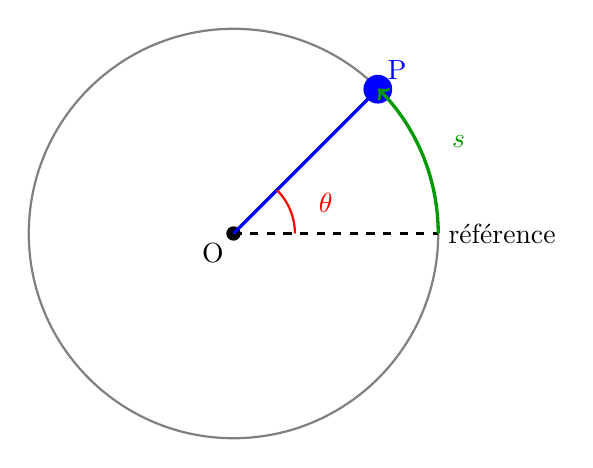
\begin{tikzpicture}[scale=1.3]
% Cercle
\draw[thick, gray] (0,0) circle (2);
% Axe de rotation
\fill (0,0) circle (2pt) node[below left] {O};
% Position initiale
\draw[thick, dashed] (0,0) -- (2,0) node[right] {référence};
% Position actuelle
\draw[very thick, blue] (0,0) -- (1.41,1.41);
\fill[blue] (1.41,1.41) circle (4pt) node[above right] {P};
% Angle
\draw[thick, red] (0.6,0) arc (0:45:0.6);
\node[red] at (0.9,0.3) {$\theta$};
% Arc
\draw[very thick, green!60!black, ->] (2,0) arc (0:45:2);
\node[green!60!black] at (2.2,0.9) {$s$};
\end{tikzpicture}
\end{center}

\subsubsection{Le radian}

Le \textbf{radian} est défini comme le rapport entre la longueur de l'arc $s$ et le rayon $r$ :

\begin{equationimportante}
\begin{equation}
\theta = \frac{s}{r} \quad \text{(en radians)}
\end{equation}
\end{equationimportante}

Un angle de 1 radian correspond à un arc de longueur égale au rayon.

\begin{center}
\renewcommand{\arraystretch}{1.4}
\begin{tabular}{|c|c|c|}
\hline
\rowcolor{bleuclair}
\textbf{Degrés} & \textbf{Radians} & \textbf{Tours} \\
\hline
$360°$ & $2\pi$ rad & 1 tour \\
\hline
$180°$ & $\pi$ rad & $\frac{1}{2}$ tour \\
\hline
$90°$ & $\frac{\pi}{2}$ rad & $\frac{1}{4}$ tour \\
\hline
$60°$ & $\frac{\pi}{3}$ rad & $\frac{1}{6}$ tour \\
\hline
$45°$ & $\frac{\pi}{4}$ rad & $\frac{1}{8}$ tour \\
\hline
$1°$ & $\frac{\pi}{180}$ rad $\approx 0,0175$ rad & -- \\
\hline
$57,3°$ & $1$ rad & -- \\
\hline
\end{tabular}
\end{center}

\begin{remarque}[title=Conversions]
\begin{align*}
\text{Degrés} \to \text{Radians} : \quad \theta_{rad} &= \theta_{deg} \times \frac{\pi}{180} \\[0.3cm]
\text{Radians} \to \text{Degrés} : \quad \theta_{deg} &= \theta_{rad} \times \frac{180}{\pi}
\end{align*}
\end{remarque}

\begin{definition}[title=Déplacement angulaire]
Le \textbf{déplacement angulaire} $\Delta\theta$ est la variation de la position angulaire :
\begin{equation}
\Delta\theta = \theta_f - \theta_i
\end{equation}

Convention de signes :
\begin{itemize}
    \item $\Delta\theta > 0$ : rotation dans le sens \textbf{antihoraire} (sens trigonométrique)
    \item $\Delta\theta < 0$ : rotation dans le sens \textbf{horaire}
\end{itemize}
\end{definition}

\subsection{Relation entre grandeurs linéaires et angulaires}

Pour un objet en rotation à une distance $r$ de l'axe, la longueur d'arc parcourue est reliée au déplacement angulaire :

\begin{equationimportante}
\begin{equation}
s = r\theta \quad \text{($\theta$ en radians)}
\end{equation}
\end{equationimportante}

\begin{exemple}{Câble enroulé sur un treuil}{}
Un treuil de rayon $\SI{15}{cm}$ effectue 5 tours complets. Quelle longueur de câble est enroulée?

\textbf{Déplacement angulaire :}
\[ \Delta\theta = 5 \text{ tours} \times 2\pi = 10\pi \text{ rad} \]

\textbf{Longueur de câble :}
\[ s = r\Delta\theta = 0,15 \times 10\pi = \SI{4,71}{m} \]
\end{exemple}

\begin{pratiqueautonome}
Un cabestan de rayon $\SI{20}{cm}$ effectue 8 tours complets pour haler un câble d'amarrage.

\begin{enumerate}[label=\alph*)]
    \item Quel est le déplacement angulaire en radians?
    \item Quelle longueur de câble a été halée?
\end{enumerate}

\espaceresolution[5cm]
\reponsepratique{a) $\Delta\theta = 16\pi \approx \SI{50,3}{rad}$ \quad b) $s \approx \SI{10,1}{m}$}
\end{pratiqueautonome}

\subsection{Vitesse angulaire}

\begin{definition}[title=Vitesse angulaire moyenne]
La \textbf{vitesse angulaire moyenne} $\omega$ est le taux de variation de la position angulaire :
\begin{equationimportante}
\begin{equation}
\omega_{moy} = \frac{\Delta\theta}{\Delta t}
\end{equation}
\end{equationimportante}

L'unité SI est le \textbf{radian par seconde} (rad/s).
\end{definition}

\begin{remarque}[title=Autres unités courantes]
\begin{itemize}
    \item \textbf{Tours par minute} (tr/min ou RPM) : très utilisé en pratique
    \item \textbf{Tours par seconde} (tr/s)
    \item \textbf{Degrés par seconde} (°/s)
\end{itemize}

\textbf{Conversions :}
\begin{align*}
\omega \text{ (rad/s)} &= \omega \text{ (RPM)} \times \frac{2\pi}{60} \\[0.3cm]
\omega \text{ (RPM)} &= \omega \text{ (rad/s)} \times \frac{60}{2\pi}
\end{align*}
\end{remarque}

\subsubsection{Relation entre vitesse linéaire et vitesse angulaire}

Un point situé à une distance $r$ de l'axe de rotation a une vitesse linéaire (tangentielle) :

\begin{equationimportante}
\begin{equation}
v = r\omega \quad \text{($\omega$ en rad/s)}
\end{equation}
\end{equationimportante}

\begin{center}
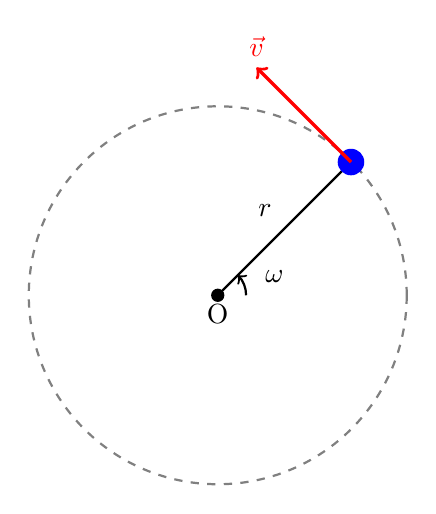
\begin{tikzpicture}[scale=1.2]
% Cercle
\draw[thick, gray, dashed] (0,0) circle (2);
% Axe
\fill (0,0) circle (2pt) node[below] {O};
% Rayon
\draw[thick] (0,0) -- (1.41,1.41);
\node at (0.5,0.9) {$r$};
% Point
\fill[blue] (1.41,1.41) circle (4pt);
% Vitesse tangentielle
\draw[very thick, red, ->] (1.41,1.41) -- (0.41,2.41) node[above] {$\vec{v}$};
% Omega
\draw[thick, ->] (0.3,0) arc (0:45:0.3);
\node at (0.6,0.2) {$\omega$};
\end{tikzpicture}
\end{center}

\begin{attention}
Plus un point est \textbf{éloigné} de l'axe de rotation, plus sa vitesse linéaire est \textbf{grande}, même si tous les points ont la même vitesse angulaire.
\end{attention}

\begin{exemple}{Vitesse en bout de pale d'hélice}{}
L'hélice d'un navire a un diamètre de $\SI{4}{m}$ et tourne à $\SI{120}{RPM}$ (tours par minute).
\begin{enumerate}[label=\alph*)]
    \item Quelle est la vitesse angulaire en rad/s?
    \item Quelle est la vitesse linéaire en bout de pale?
\end{enumerate}

\textbf{a) Vitesse angulaire :}
\[ \omega = \SI{120}{RPM} \times \frac{2\pi \text{ rad}}{\SI{1}{tour}} \times \frac{\SI{1}{min}}{\SI{60}{s}} = \SI{120}{RPM} \times \frac{2\pi}{60} \frac{\text{rad/s}}{\text{RPM}} = \SI{12,6}{rad/s} \]

\textbf{b) Vitesse en bout de pale :}

Le rayon est $r = \dfrac{d}{2} = \dfrac{\SI{4}{m}}{2} = \SI{2}{m}$.
\[ v = r\omega = \SI{2}{m} \times \SI{12,6}{rad/s} = \SI{25,1}{m/s} \]

Conversion en km/h : $v = \SI{25,1}{m/s} \times \dfrac{\SI{3,6}{km/h}}{\SI{1}{m/s}} = \SI{90}{km/h}$

Les extrémités des pales se déplacent à près de $\SI{90}{km/h}$!
\end{exemple}

\begin{pratiqueautonome}
L'hélice d'un navire a un diamètre de $\SI{5}{m}$ et tourne à $\SI{90}{RPM}$.

\begin{enumerate}[label=\alph*)]
    \item Calculez la vitesse angulaire en rad/s.
    \item Calculez la vitesse linéaire en bout de pale. Exprimez votre réponse en m/s et en km/h.
\end{enumerate}

\espaceresolution[5cm]
\reponsepratique{a) $\omega \approx \SI{9,4}{rad/s}$ \quad b) $v \approx \SI{23,6}{m/s} \approx \SI{85}{km/h}$}
\end{pratiqueautonome}

\subsection{Accélération angulaire}

\begin{definition}[title=Accélération angulaire moyenne]
L'\textbf{accélération angulaire moyenne} $\alpha$ est le taux de variation de la vitesse angulaire :
\begin{equationimportante}
\begin{equation}
\alpha_{moy} = \frac{\Delta\omega}{\Delta t}
\end{equation}
\end{equationimportante}

L'unité SI est le \textbf{radian par seconde carrée} (rad/s²).
\end{definition}

\subsubsection{Accélération tangentielle}

L'accélération tangentielle est due à la variation du \textbf{module} de la vitesse :

\begin{equationimportante}
\begin{equation}
a_t = r\alpha
\end{equation}
\end{equationimportante}

\begin{exemple}{Démarrage d'un treuil}{}
Un treuil de rayon $\SI{20}{cm}$ part du repos et atteint une vitesse de $\SI{60}{RPM}$ en $\SI{5}{s}$.
\begin{enumerate}[label=\alph*)]
    \item Quelle est son accélération angulaire?
    \item Quelle est l'accélération tangentielle du câble?
\end{enumerate}

\textbf{a) Accélération angulaire :}

Conversion de la vitesse finale :
\[ \omega_f = \SI{60}{RPM} \times \frac{2\pi}{60} \frac{\text{rad/s}}{\text{RPM}} = \SI{6,28}{rad/s} \]

Calcul de l'accélération :
\[ \alpha = \frac{\omega_f - \omega_i}{\Delta t} = \frac{\SI{6,28}{rad/s} - \SI{0}{rad/s}}{\SI{5}{s}} = \SI{1,26}{rad/s^2} \]

\textbf{b) Accélération tangentielle :}

Conversion du rayon : $r = \SI{20}{cm} = \SI{0,20}{m}$
\[ a_t = r\alpha = \SI{0,20}{m} \times \SI{1,26}{rad/s^2} = \SI{0,25}{m/s^2} \]
\end{exemple}

\subsection{Équations du mouvement circulaire uniformément accéléré}

Lorsque l'accélération angulaire $\alpha$ est \textbf{constante}, on peut utiliser des équations analogues à celles du MRUA :

\begin{equationimportante}
\textbf{Équations du mouvement circulaire uniformément accéléré}
\begin{align}
\omega_f &= \omega_i + \alpha \Delta t \\[0.3cm]
\Delta\theta &= \frac{1}{2}(\omega_i + \omega_f)\Delta t \\[0.3cm]
\Delta\theta &= \omega_i \Delta t + \frac{1}{2}\alpha(\Delta t)^2 \\[0.3cm]
\omega_f^2 &= \omega_i^2 + 2\alpha\Delta\theta
\end{align}
\end{equationimportante}

\subsection{Analogie translation-rotation}

\begin{center}
\renewcommand{\arraystretch}{1.6}
\begin{tabular}{|c|c|c|}
\hline
\rowcolor{bleuclair}
\textbf{Grandeur} & \textbf{Translation} & \textbf{Rotation} \\
\hline
Position & $x$ (m) & $\theta$ (rad) \\
\hline
Déplacement & $\Delta x$ (m) & $\Delta\theta$ (rad) \\
\hline
Vitesse & $v = \dfrac{\Delta x}{\Delta t}$ (m/s) & $\omega = \dfrac{\Delta\theta}{\Delta t}$ (rad/s) \\
\hline
Accélération & $a = \dfrac{\Delta v}{\Delta t}$ (m/s²) & $\alpha = \dfrac{\Delta\omega}{\Delta t}$ (rad/s²) \\
\hline
\hline
\multirow{4}{*}{Équations MRUA} & $v_f = v_i + a\Delta t$ & $\omega_f = \omega_i + \alpha\Delta t$ \\
\cline{2-3}
& $\Delta x = \frac{1}{2}(v_i + v_f)\Delta t$ & $\Delta\theta = \frac{1}{2}(\omega_i + \omega_f)\Delta t$ \\
\cline{2-3}
& $\Delta x = v_i\Delta t + \frac{1}{2}a(\Delta t)^2$ & $\Delta\theta = \omega_i\Delta t + \frac{1}{2}\alpha(\Delta t)^2$ \\
\cline{2-3}
& $v_f^2 = v_i^2 + 2a\Delta x$ & $\omega_f^2 = \omega_i^2 + 2\alpha\Delta\theta$ \\
\hline
\hline
\multicolumn{3}{|c|}{\textbf{Relations entre grandeurs linéaires et angulaires}} \\
\hline
\multicolumn{3}{|c|}{$s = r\theta$ \quad\quad $v = r\omega$ \quad\quad $a_t = r\alpha$} \\
\hline
\end{tabular}
\end{center}

\begin{remarque}[title=Puissance de l'analogie]
Si vous maîtrisez les équations du MRUA en translation, vous maîtrisez automatiquement celles de la rotation! Il suffit de remplacer :
\begin{itemize}
    \item $x \to \theta$
    \item $v \to \omega$
    \item $a \to \alpha$
\end{itemize}
\end{remarque}

\subsection{Applications maritimes}

\begin{exemple}{Freinage d'une hélice}{}
L'hélice d'un navire tourne à $\SI{150}{RPM}$. Lors de l'arrêt des machines, elle décélère uniformément et s'arrête après avoir effectué 20 tours.
\begin{enumerate}[label=\alph*)]
    \item Quelle est la décélération angulaire?
    \item Combien de temps dure le freinage?
\end{enumerate}

\textbf{Données :}
\begin{itemize}
    \item $\omega_i = 150 \times \frac{2\pi}{60} = \SI{15,7}{rad/s}$
    \item $\omega_f = \SI{0}{rad/s}$
    \item $\Delta\theta = 20 \times 2\pi = \SI{125,7}{rad}$
\end{itemize}

\textbf{a) Décélération angulaire :}
\begin{align*}
\omega_f^2 &= \omega_i^2 + 2\alpha\Delta\theta \\
0 &= 15,7^2 + 2\alpha(125,7) \\
\alpha &= \frac{-246,5}{251,4} = \SI{-0,98}{rad/s^2}
\end{align*}

\textbf{b) Temps de freinage :}
\[ \Delta t = \frac{\omega_f - \omega_i}{\alpha} = \frac{0 - 15,7}{-0,98} = \SI{16,0}{s} \]
\end{exemple}

\begin{exemple}{Radar rotatif}{}
Un radar de navigation effectue un balayage complet toutes les $\SI{3}{s}$.
\begin{enumerate}[label=\alph*)]
    \item Quelle est sa vitesse angulaire en rad/s et en RPM?
    \item Si l'antenne a une longueur de $\SI{1,5}{m}$, quelle est la vitesse linéaire de son extrémité?
\end{enumerate}

\textbf{a) Vitesse angulaire :}
\[ \omega = \frac{2\pi}{3} = \SI{2,09}{rad/s} = 2,09 \times \frac{60}{2\pi} = \SI{20}{RPM} \]

\textbf{b) Vitesse linéaire :}
\[ v = r\omega = 1,5 \times 2,09 = \SI{3,14}{m/s} \]
\end{exemple}

\begin{exemple}{Cabestan (exemple de calcul complet)}{}
Un cabestan de rayon $\SI{25}{cm}$ est utilisé pour haler un câble. Il démarre du repos et accélère à $\SI{0,5}{rad/s^2}$ pendant $\SI{4}{s}$, puis maintient une vitesse constante.
\begin{enumerate}[label=\alph*)]
    \item Quelle vitesse angulaire atteint-il?
    \item Combien de tours effectue-t-il pendant l'accélération?
    \item Quelle longueur de câble est halée pendant les 10 premières secondes?
\end{enumerate}

\textbf{a) Vitesse angulaire finale :}
\[ \omega_f = \omega_i + \alpha\Delta t = 0 + 0,5 \times 4 = \SI{2}{rad/s} \]

En RPM : $\omega_f = 2 \times \frac{60}{2\pi} = \SI{19,1}{RPM}$

\textbf{b) Déplacement angulaire pendant l'accélération :}
\[ \Delta\theta = \omega_i\Delta t + \frac{1}{2}\alpha(\Delta t)^2 = 0 + \frac{1}{2}(0,5)(4)^2 = \SI{4}{rad} \]

Nombre de tours : $\frac{4}{2\pi} = 0,64$ tour

\textbf{c) Longueur de câble halée en 10 s :}

Phase 1 (0 à 4 s, accélération) : $\Delta\theta_1 = \SI{4}{rad}$

Phase 2 (4 à 10 s, vitesse constante) : 
\[ \Delta\theta_2 = \omega \times \Delta t = 2 \times 6 = \SI{12}{rad} \]

Total : $\Delta\theta_{total} = 4 + 12 = \SI{16}{rad}$

Longueur de câble :
\[ s = r\Delta\theta = 0,25 \times 16 = \SI{4}{m} \]
\end{exemple}


% 5. Compléments
% =============================================================================
\section*{Compl\'ement : Vitesse relative}
\addcontentsline{toc}{section}{Compl\'ement : Vitesse relative}
% =============================================================================

En navigation, il est souvent n\'ecessaire de tenir compte du \textbf{courant} ou du \textbf{vent} pour d\'eterminer la vitesse r\'eelle d'un navire par rapport au fond marin ou \`a un point fixe.

\begin{definition}[title=Vitesse relative]
La \textbf{vitesse relative} d'un objet A par rapport \`a un objet B est la vitesse de A telle que la percevrait un observateur situ\'e sur B :
\begin{equation}
\vec{v}_{A/B} = \vec{v}_A - \vec{v}_B
\end{equation}
\end{definition}

\begin{remarque}[title=Terminologie maritime]
\begin{itemize}
    \item \textbf{Vitesse surface} ($\vec{v}_{surface}$) : vitesse du navire par rapport \`a l'eau (mesur\'ee par le loch)
    \item \textbf{Vitesse fond} ($\vec{v}_{fond}$) : vitesse du navire par rapport au fond marin (mesur\'ee par GPS)
    \item \textbf{Courant} ($\vec{v}_{courant}$) : vitesse de l'eau par rapport au fond
\end{itemize}

La relation fondamentale est :
\begin{equation}
\vec{v}_{fond} = \vec{v}_{surface} + \vec{v}_{courant}
\end{equation}
\end{remarque}

\begin{exemple}{Navire contre le courant}{navire-contre-courant}
Un cargo navigue vers l'est \`a $\SI{12}{n\oe{}uds}$ (vitesse surface). Le courant porte vers l'ouest \`a $\SI{3}{n\oe{}uds}$.

Quelle est la vitesse fond du cargo?

\textbf{Solution :}

En prenant l'est comme direction positive :
\begin{itemize}
    \item $v_{surface} = +\SI{12}{n\oe{}uds}$ (vers l'est)
    \item $v_{courant} = -\SI{3}{n\oe{}uds}$ (vers l'ouest)
\end{itemize}

\[ v_{fond} = v_{surface} + v_{courant} = 12 + (-3) = \SI{9}{n\oe{}uds} \text{ vers l'est} \]

Le navire avance effectivement \`a $\SI{9}{n\oe{}uds}$ par rapport au fond.
\end{exemple}

\begin{exemple}{Travers\'ee avec courant lat\'eral --- Décomposition vectorielle}{traversee-courant-lateral}
Un traversier doit rejoindre un quai situ\'e exactement au nord, \`a $\SI{2}{km}$. Sa vitesse propre (surface) est de $\SI{10}{n\oe{}uds}$, mais un courant de $\SI{3}{n\oe{}uds}$ porte vers l'est.

\textbf{Problème :} Si le capitaine pointe directement vers le nord, le navire dérivera vers l'est. Pour atteindre le quai, il doit \textbf{compenser} en pointant légèrement vers l'ouest.

\begin{center}
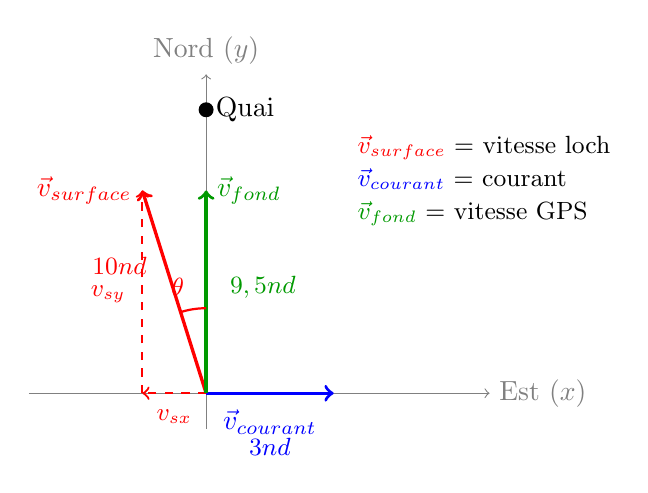
\begin{tikzpicture}[scale=0.9]
% Axes
\draw[gray, ->] (-2.5,0) -- (4,0) node[right] {Est ($x$)};
\draw[gray, ->] (0,-0.5) -- (0,4.5) node[above] {Nord ($y$)};
% Courant (horizontal vers l'est)
\draw[very thick, blue, ->] (0,0) -- (1.8,0);
\node[blue, below] at (0.9,-0.1) {$\vec{v}_{courant}$};
\node[blue, below] at (0.9,-0.5) {\small $\SI{3}{nd}$};
% Vitesse surface (inclinée pour compenser) - angle θ ouest du nord
% sin(17.46$^\circ$) = 0.3, cos(17.46$^\circ$) = 0.954
\draw[very thick, red, ->] (0,0) -- ({-3*sin(17.46)},{3*cos(17.46)}) node[left] {$\vec{v}_{surface}$};
\node[red, left] at (-0.7,1.8) {\small $\SI{10}{nd}$};
% Composantes de la vitesse surface (en pointillés)
\draw[red, dashed, thick, ->] (0,0) -- ({-3*sin(17.46)},0);
\node[red, below] at ({-0.5*3*sin(17.46)},-0.1) {\small $v_{sx}$};
\draw[red, dashed, thick, ->] ({-3*sin(17.46)},0) -- ({-3*sin(17.46)},{3*cos(17.46)});
\node[red, left] at ({-3*sin(17.46)-0.1},1.4) {\small $v_{sy}$};
% Vitesse fond (résultante vers le nord)
\draw[very thick, green!60!black, ->] (0,0) -- (0,{3*cos(17.46)}) node[right] {$\vec{v}_{fond}$};
\node[green!60!black, right] at (0.2,1.5) {\small $\SI{9,5}{nd}$};
% Angle
\draw[thick, red] (0,1.2) arc (90:107.46:1.2);
\node[red] at (-0.4,1.5) {\small $\theta$};
% Point d'arrivée
\fill (0,4) circle (3pt) node[right] {Quai};
% Légende
\node[align=left, anchor=west] at (2,3) {\small \textcolor{red}{$\vec{v}_{surface}$} = vitesse loch\\
\small \textcolor{blue}{$\vec{v}_{courant}$} = courant\\
\small \textcolor{green!60!black}{$\vec{v}_{fond}$} = vitesse GPS};
\end{tikzpicture}
\end{center}

\textbf{Analyse par décomposition vectorielle :}

Pour que $\vec{v}_{fond}$ soit dirigée exactement vers le nord, sa composante $x$ doit être nulle :
\begin{align*}
v_{fond,x} &= v_{surface,x} + v_{courant,x} = 0 \\
-v_{surface}\sin\theta + v_{courant} &= 0
\end{align*}

D'où l'\textbf{angle de compensation} :
\[ \sin\theta = \frac{v_{courant}}{v_{surface}} = \frac{3}{10} = 0{,}3 \quad \Rightarrow \quad \boxed{\theta = 17{,}5^\circ \text{ ouest du nord}} \]

\textbf{Vitesse fond r\'esultante} (composante $y$) :
\[ v_{fond} = v_{fond,y} = v_{surface}\cos\theta = 10 \times \cos(17{,}5^\circ) = \boxed{\SI{9{,}5}{n\oe{}uds}} \]

\textbf{Vérification} par le théorème de Pythagore :
\[ v_{surface}^2 = v_{fond}^2 + v_{courant}^2 \quad \Rightarrow \quad 10^2 = 9{,}5^2 + 3^2 = 90{,}25 + 9 = 99{,}25 \approx 100 \quad \checkmark \]
\end{exemple}

\begin{attention}
La vitesse relative est un concept vectoriel. En 2D, il faut d\'ecomposer les vitesses en composantes et les additionner vectoriellement. Ce sujet sera approfondi dans le cours de navigation.
\end{attention}

% 6. Résumé et compétences
% =============================================================================
% CHAPITRE 1 - CINÉMATIQUE
% Partie 7 : Résumé, compétences et exercices
% Version maritime pour l'IMQ
% =============================================================================

% =============================================================================
\section*{Résumé du chapitre}
\addcontentsline{toc}{section}{Résumé}
% =============================================================================

\begin{center}
\renewcommand{\arraystretch}{2.0}
\begin{longtable}{|L{8cm}|C{6cm}|}
\hline
\rowcolor{bleuclair}
\textbf{Concept} & \textbf{Formule / Définition} \\
\hline
\endfirsthead
\hline
\rowcolor{bleuclair}
\textbf{Concept} & \textbf{Formule / Définition} \\
\hline
\endhead

La \textbf{cinématique} est la branche de la mécanique qui \textbf{décrit} le mouvement des corps, sans s'intéresser à ses causes. & Description qualitative et mathématique du mouvement \\
\hline

Le \textbf{déplacement} est la variation de position. C'est une grandeur vectorielle (avec signe en 1D). & $\Delta x = x_f - x_i$ \\
\hline

La \textbf{distance parcourue} est la longueur totale du trajet. C'est une grandeur scalaire (toujours $\geq 0$). & $d = $ longueur du trajet \\
\hline

La \textbf{vitesse moyenne} est le rapport entre le déplacement et l'intervalle de temps. & $v_{moy} = \dfrac{\Delta x}{\Delta t}$ \\
\hline

La \textbf{vitesse scalaire moyenne} est le rapport entre la distance parcourue et l'intervalle de temps. & $v_{scalaire} = \dfrac{d}{\Delta t}$ \\
\hline

La \textbf{vitesse instantanée} est la vitesse à un instant précis. Graphiquement, c'est la pente de la tangente à $x(t)$. & $v = \text{pente de la tangente à } x(t)$ \\
\hline

L'\textbf{accélération moyenne} est le rapport entre la variation de vitesse et l'intervalle de temps. & $a_{moy} = \dfrac{\Delta v}{\Delta t}$ \\
\hline

L'\textbf{accélération instantanée} est l'accélération à un instant précis. C'est la pente de la tangente à $v(t)$. & $a = \text{pente de la tangente à } v(t)$ \\
\hline

\textbf{Équations du MRUA} (mouvement à accélération constante) & 
$v_f = v_i + a\Delta t$ \newline
$v_{moy} = \dfrac{v_i + v_f}{2}$ \newline
$\Delta x = \dfrac{1}{2}(v_i + v_f)\Delta t$ \newline
$\Delta x = v_i\Delta t + \dfrac{1}{2}a(\Delta t)^2$ \newline
$v_f^2 = v_i^2 + 2a\Delta x$ \\
\hline

\textbf{Conversion maritime} : Le n\oe{}ud est l'unité de vitesse en navigation. & $\SI{1}{\knots} = \SI{1,852}{km/h} = \SI{0,5144}{m/s}$ \\
\hline

\textbf{Mouvement rectiligne uniforme (MRU)} : mouvement en ligne droite à vitesse constante. & $\Delta x = v \cdot \Delta t$ \\
\hline

\textbf{Chute libre} : mouvement sous la seule action de la gravité (MRUA vertical). & $g = \SI{9,81}{m/s^2}$ (vers le bas) \\
\hline

\textbf{Mouvement en 2D} : décomposer en $x$ et $y$, traiter séparément, relier par le temps $\Delta t$. & $v_x = v\cos\theta$ \newline $v_y = v\sin\theta$ \\
\hline

\textbf{Projectile} : en $x$ c'est un MRU, en $y$ c'est une chute libre. & $a_x = 0$ \newline $a_y = -g$ \\
\hline

\textbf{Cinématique de rotation} : analogie complète avec la translation. & $\theta = \dfrac{s}{r}$ \newline $\omega = \dfrac{\Delta\theta}{\Delta t}$ \newline $\alpha = \dfrac{\Delta\omega}{\Delta t}$ \\
\hline

\textbf{Relations linéaire-angulaire} & $s = r\theta$ \newline $v = r\omega$ \newline $a_t = r\alpha$ \\
\hline

\textbf{Équations rotation} (accélération angulaire constante) & 
$\omega_f = \omega_i + \alpha\Delta t$ \newline
$\Delta\theta = \omega_i\Delta t + \dfrac{1}{2}\alpha(\Delta t)^2$ \newline
$\omega_f^2 = \omega_i^2 + 2\alpha\Delta\theta$ \\
\hline

\end{longtable}
\end{center}

% =============================================================================
\section*{Compétences}
\addcontentsline{toc}{section}{Compétences}
% =============================================================================

À la fin de ce chapitre, vous devriez être en mesure de :

\begin{center}
\renewcommand{\arraystretch}{1.4}
\begin{tabular}{|L{10cm}|C{1cm}|C{1cm}|C{1cm}|C{1cm}|}
\hline
\rowcolor{bleuclair}
\textbf{Compétence} & \rotatebox{90}{\textbf{Difficile}} & \rotatebox{90}{\textbf{Familier}} & \rotatebox{90}{\textbf{Minimum}} & \rotatebox{90}{\textbf{Maîtrise}} \\
\hline
\multicolumn{5}{|l|}{\cellcolor{gray!20}\textbf{Cinématique de translation (1D)}} \\
\hline
Expliquer ce qu'est la cinématique (description du mouvement) & & & & \\
\hline
Différencier un déplacement et une distance parcourue & & & & \\
\hline
Calculer la vitesse moyenne à partir de données ou d'un graphique & & & & \\
\hline
Calculer la vitesse scalaire moyenne & & & & \\
\hline
Interpréter un graphique position-temps $x(t)$ & & & & \\
\hline
Déterminer la vitesse instantanée à partir d'un graphique & & & & \\
\hline
Calculer l'accélération moyenne & & & & \\
\hline
Interpréter un graphique vitesse-temps $v(t)$ & & & & \\
\hline
Choisir et appliquer les équations du MRUA & & & & \\
\hline
\multicolumn{5}{|l|}{\cellcolor{gray!20}\textbf{Chute libre et projectile (2D)}} \\
\hline
Appliquer les équations du MRUA à la chute libre & & & & \\
\hline
Résoudre des problèmes de chute libre (objet lâché ou lancé) & & & & \\
\hline
Décomposer la vitesse initiale d'un projectile en composantes & & & & \\
\hline
Résoudre des problèmes de projectile en 2D & & & & \\
\hline
\multicolumn{5}{|l|}{\cellcolor{gray!20}\textbf{Cinématique de rotation}} \\
\hline
Convertir des angles entre degrés, radians et tours & & & & \\
\hline
Calculer la vitesse angulaire et convertir entre rad/s et RPM & & & & \\
\hline
Utiliser les relations $s = r\theta$, $v = r\omega$, $a_t = r\alpha$ & & & & \\
\hline
Appliquer les équations du mouvement circulaire uniformément accéléré & & & & \\
\hline
\multicolumn{5}{|l|}{\cellcolor{gray!20}\textbf{Applications}} \\
\hline
Convertir entre les unités SI et les unités maritimes (n\oe{}uds, NM) & & & & \\
\hline
Résoudre des problèmes de navigation impliquant la cinématique & & & & \\
\hline
\end{tabular}
\end{center}


% 7. Exercices (optionnel - peut être inclus séparément)
% % =============================================================================
\section*{Exercices}
\addcontentsline{toc}{section}{Exercices}
% =============================================================================

\begin{remarque}[title=Niveaux de difficulté]
\begin{itemize}
    \item[$\star$] Application directe d'une formule
    \item[$\star\star$] Problème à plusieurs étapes ou avec conversion
    \item[$\star\star\star$] Problème complexe ou piège conceptuel
\end{itemize}
\end{remarque}

% -----------------------------------------------------------------------------
\subsection*{Position et déplacement}
% -----------------------------------------------------------------------------

\begin{enumerate}
\item[$\star$] \textbf{1.} Un navire-citerne part du terminal A (position $x = 0$), se rend au terminal B situé à $\SI{15}{km}$ à l'est, puis revient au terminal C situé à $\SI{8}{km}$ à l'est de A.
\begin{enumerate}[label=\alph*)]
    \item Quelle est la distance totale parcourue?
    \item Quel est le déplacement du navire?
\end{enumerate}

\item[$\star$] \textbf{2.} Un remorqueur effectue les déplacements suivants dans un port : $\SI{200}{m}$ vers l'est, $\SI{150}{m}$ vers l'ouest, puis $\SI{300}{m}$ vers l'est. Calculez la distance parcourue et le déplacement net.

\item[$\star\star$] \textbf{3.} Un patrouilleur part de sa base, navigue $\SI{12}{km}$ vers l'est puis $\SI{5}{km}$ vers le nord.
\begin{enumerate}[label=\alph*)]
    \item Quelle est la distance totale parcourue?
    \item Quel est le module du déplacement? (Utilisez le théorème de Pythagore)
\end{enumerate}

\item[$\star\star\star$] \textbf{4.} \textbf{Vrai ou faux?} Justifiez chaque réponse.
\begin{enumerate}[label=\alph*)]
    \item Le déplacement est toujours inférieur ou égal à la distance parcourue.
    \item Si un navire revient à son point de départ, sa vitesse moyenne est nulle mais sa vitesse scalaire moyenne ne l'est pas.
    \item Le déplacement dépend du trajet emprunté.
\end{enumerate}
\end{enumerate}

% -----------------------------------------------------------------------------
\subsection*{Vitesse moyenne et scalaire}
% -----------------------------------------------------------------------------

\begin{enumerate}[resume]
\item[$\star$] \textbf{5.} Un traversier effectue la traversée Rimouski--Forestville ($\SI{25}{km}$) en $\SI{55}{min}$. Calculez sa vitesse moyenne en km/h, en m/s et en n\oe{}uds.

\item[$\star$] \textbf{6.} Un cargo parcourt $\SI{450}{milles nautiques}$ en 30 heures. Quelle est sa vitesse moyenne en n\oe{}uds et en m/s?

\item[$\star\star$] \textbf{7.} Un patrouilleur des garde-côtes part de sa base, parcourt $\SI{40}{NM}$ vers le nord à $\SI{20}{n\oe{}uds}$, puis revient à sa base à $\SI{15}{n\oe{}uds}$.
\begin{enumerate}[label=\alph*)]
    \item Quel est le temps total de la patrouille?
    \item Quelle est la vitesse moyenne sur l'ensemble du trajet?
    \item Quelle est la vitesse scalaire moyenne?
\end{enumerate}

\item[$\star\star$] \textbf{8.} Un vraquier effectue un trajet de $\SI{1200}{NM}$. Il navigue à $\SI{12}{n\oe{}uds}$ pendant les 20 premières heures, puis à $\SI{15}{n\oe{}uds}$ pour le reste du trajet. Quelle est sa vitesse scalaire moyenne?

\item[$\star\star\star$] \textbf{9.} \textbf{Question piège!} Un navire parcourt la \textit{première moitié} d'un trajet à $\SI{10}{n\oe{}uds}$ et la \textit{seconde moitié} à $\SI{20}{n\oe{}uds}$. 
\begin{enumerate}[label=\alph*)]
    \item Quelle est sa vitesse scalaire moyenne? 
    \item Expliquez pourquoi ce n'est \textbf{pas} $\SI{15}{n\oe{}uds}$.
\end{enumerate}

\item[$\star\star\star$] \textbf{10.} Un autre navire parcourt la \textit{première moitié du temps} à $\SI{10}{n\oe{}uds}$ et la \textit{seconde moitié du temps} à $\SI{20}{n\oe{}uds}$. Quelle est sa vitesse scalaire moyenne? Comparez avec l'exercice précédent.

% --- Problèmes de rencontre/rattrapage MRU ---

\item[$\star\star$] \textbf{11.} Deux trains partent simultanément de gares situées à $\SI{200}{km}$ l'une de l'autre et roulent l'un vers l'autre. Le train A roule à $\SI{90}{km/h}$ et le train B à $\SI{110}{km/h}$.
\begin{enumerate}[label=\alph*)]
    \item Après combien de temps se croiseront-ils?
    \item À quelle distance de la gare de A se trouvera le point de rencontre?
\end{enumerate}

\item[$\star\star$] \textbf{12.} Une voiture quitte Montréal à 8h00 et roule vers Québec à $\SI{100}{km/h}$. Une autre voiture quitte Québec à 9h00 et roule vers Montréal à $\SI{110}{km/h}$. Les deux villes sont séparées de $\SI{250}{km}$.
\begin{enumerate}[label=\alph*)]
    \item À quelle heure les deux voitures se croisent-elles?
    \item À quelle distance de Montréal se trouvent-elles à ce moment?
\end{enumerate}

\item[$\star\star$] \textbf{13.} Un cycliste roule vers le nord à $\SI{25}{km/h}$. Un coureur, situé $\SI{500}{m}$ au nord du cycliste, court dans la même direction à $\SI{12}{km/h}$.
\begin{enumerate}[label=\alph*)]
    \item Après combien de temps le cycliste rattrape-t-il le coureur?
    \item Quelle distance chacun a-t-il parcourue?
\end{enumerate}

\end{enumerate}

% -----------------------------------------------------------------------------
\subsection*{Graphiques}
% -----------------------------------------------------------------------------

\begin{enumerate}[resume]
\item[$\star\star$] \textbf{14.} Le graphique suivant montre la position d'un navire en fonction du temps :

\begin{center}
\begin{tikzpicture}[scale=0.6]
\draw[axe, thick] (0,0) -- (8,0) node[right] {$t$ (h)};
\draw[axe, thick] (0,0) -- (0,5) node[above] {$x$ (NM)};
\foreach \x in {1,2,3,4,5,6,7} {\draw (\x,0.1) -- (\x,-0.1) node[below] {\x};}
\foreach \y in {1,2,3,4} {\draw (0.1,\y) -- (-0.1,\y) node[left] {\pgfmathparse{int(\y*20)}\pgfmathresult};}
\draw[very thick, blue] (0,0) -- (2,2) -- (4,2) -- (7,4);
\end{tikzpicture}
\end{center}

\begin{enumerate}[label=\alph*)]
    \item Décrivez qualitativement le mouvement du navire.
    \item Calculez la vitesse entre $t = 0$ et $t = 2$ h.
    \item Le navire est-il à l'arrêt à un certain moment? Si oui, quand?
    \item Quelle est la vitesse moyenne sur l'ensemble du trajet (0 à 7 h)?
\end{enumerate}

\item[$\star\star$] \textbf{15.} Le graphique suivant montre la vitesse d'un cargo en fonction du temps :

\begin{center}
\begin{tikzpicture}[scale=0.6]
\draw[axe, thick] (0,0) -- (8,0) node[right] {$t$ (min)};
\draw[axe, thick] (0,0) -- (0,5) node[above] {$v$ (m/s)};
\foreach \x in {2,4,6,8,10,12,14} {\draw (\x/2,0.1) -- (\x/2,-0.1) node[below] {\x};}
\foreach \y in {1,2,3,4} {\draw (0.1,\y) -- (-0.1,\y) node[left] {\y};}
\draw[very thick, blue] (0,0) -- (2,4) -- (5,4) -- (7,0);
\end{tikzpicture}
\end{center}

\begin{enumerate}[label=\alph*)]
    \item Calculez l'accélération pendant les 4 premières minutes.
    \item Pendant quelle phase le navire est-il en MRU?
    \item Calculez la distance totale parcourue (aire sous la courbe).
\end{enumerate}

\item[$\star\star\star$] \textbf{16.} \textbf{Expliquez} pourquoi, sur un graphique position-temps $x(t)$, une pente négative signifie que l'objet se déplace dans le sens négatif, et non pas qu'il recule nécessairement.

\item[$\star\star$] \textbf{17.} Un navire-citerne effectue une manœuvre d'approche. Le graphique suivant montre sa vitesse en fonction du temps :

\begin{center}
\begin{tikzpicture}[scale=0.6]
\draw[axe, thick] (0,0) -- (10,0) node[right] {$t$ (min)};
\draw[axe, thick] (0,0) -- (0,5) node[above] {$v$ (m/s)};
\foreach \x in {2,4,6,8,10,12,14,16,18} {\draw (\x/2,0.1) -- (\x/2,-0.1) node[below] {\small\x};}
\foreach \y in {1,2,3,4} {\draw (0.1,\y) -- (-0.1,\y) node[left] {\y};}
\draw[very thick, blue] (0,3) -- (2,3) -- (4,4) -- (6,4) -- (9,0);
\fill[blue] (0,3) circle (2pt);
\fill[blue] (2,3) circle (2pt);
\fill[blue] (4,4) circle (2pt);
\fill[blue] (6,4) circle (2pt);
\fill[blue] (9,0) circle (2pt);
\end{tikzpicture}
\end{center}

\begin{enumerate}[label=\alph*)]
    \item Décrivez qualitativement les différentes phases du mouvement.
    \item Calculez l'accélération pendant la phase d'accélération (entre $t = 4$ et $t = 8$ min).
    \item Calculez l'accélération pendant la phase de freinage.
    \item Calculez la distance totale parcourue pendant toute la manœuvre (aire sous la courbe).
    \item \textbf{Tracez} le graphique $a(t)$ correspondant à ce mouvement.
\end{enumerate}

\item[$\star\star\star$] \textbf{18.} Un cargo quitte le port de Montréal. Voici le graphique de son accélération en fonction du temps pendant les 10 premières minutes :

\begin{center}
\begin{tikzpicture}[scale=0.7]
\draw[axe, thick] (0,0) -- (8,0) node[right] {$t$ (min)};
\draw[axe, thick] (0,-1.5) -- (0,3) node[above] {$a$ ($\times 10^{-2}$ m/s²)};
% Graduations temps
\foreach \x in {2,4,6,8,10} {\draw (\x*0.7,0.1) -- (\x*0.7,-0.1) node[below] {\small\x};}
% Graduations accélération
\draw (0.1,2) -- (-0.1,2) node[left] {\small 2};
\draw (0.1,1) -- (-0.1,1) node[left] {\small 1};
\draw (0.1,-1) -- (-0.1,-1) node[left] {\small $-1$};
% Courbe: a = 0.02 de 0 à 4 min, puis a = 0 de 4 à 8 min, puis a = -0.01 de 8 à 10 min
\draw[very thick, blue] (0,2) -- (2.8,2);
\draw[very thick, blue, dashed] (2.8,2) -- (2.8,0);
\draw[very thick, blue] (2.8,0) -- (5.6,0);
\draw[very thick, blue, dashed] (5.6,0) -- (5.6,-1);
\draw[very thick, blue] (5.6,-1) -- (7,-1);
\fill[blue] (0,2) circle (2pt);
\fill[blue] (2.8,2) circle (2pt);
\fill[blue] (2.8,0) circle (2pt);
\fill[blue] (5.6,0) circle (2pt);
\fill[blue] (5.6,-1) circle (2pt);
\fill[blue] (7,-1) circle (2pt);
\end{tikzpicture}
\end{center}

Le cargo part du repos ($v_0 = 0$).
\begin{enumerate}[label=\alph*)]
    \item Calculez la vitesse du cargo à $t = 4$ min.
    \item Calculez la vitesse du cargo à $t = 8$ min.
    \item Calculez la vitesse du cargo à $t = 10$ min.
    \item \textbf{Tracez} le graphique $v(t)$ correspondant.
\end{enumerate}

\item[$\star\star\star$] \textbf{19.} Un traversier effectue la traversée entre deux quais. Voici le graphique de sa position en fonction du temps :

\begin{center}
\begin{tikzpicture}[x=0.7cm,y=1cm, scale=0.75]
\draw[axe, thick] (0,0) -- (10.5,0) node[right] {$t$ (min)};
\draw[axe, thick] (0,0) -- (0,4.5) node[above] {$x$ (m)};

% Graduations temps
\foreach \x in {0,2,4,6,8,10} {\draw (\x,0.1) -- (\x,-0.1) node[below] {\small\x};}
% Graduations position (1 unité = 500 m)
\foreach \y in {0,1,2,3,4} {\draw (0.1,\y) -- (-0.1,\y) node[left] {\pgfmathparse{int(\y*500)}\pgfmathresult};}

% Phase 1 : accélération (courbe concave vers le haut) de 0 à 3 min
\draw[very thick, blue, domain=0:3, samples=60] plot (\x, {0.1*\x*\x});

% Phase 2 : vitesse constante (droite) de 3 à 7 min
\draw[very thick, blue] (3,0.9) -- (7,3.3);

% Phase 3 : freinage (courbe concave vers le bas) de 7 à 10 min
\draw[very thick, blue, domain=7:10, samples=80] plot (\x, {3.3 + 0.6*(\x-7) - 0.067*(\x-7)*(\x-7)});

% Points repères
\fill[blue] (0,0) circle (2pt);
\fill[blue] (3,0.9) circle (2pt);
\fill[blue] (7,3.3) circle (2pt);
\fill[blue] (10,3.9) circle (2pt);

% Annotations
\node[above right, blue, font=\footnotesize] at (1.5,0.2) {Phase 1};
\node[above, blue, font=\footnotesize] at (5,2.1) {Phase 2};
\node[above left, blue, font=\footnotesize] at (8.5,3.6) {Phase 3};
\end{tikzpicture}
\end{center}

\begin{enumerate}[label=\alph*)]
    \item Identifiez les trois phases du mouvement (accélération, vitesse constante, freinage).
    \item Estimez graphiquement la vitesse maximale atteinte (pente de la partie linéaire).
    \item Le traversier est-il à l'arrêt au début et à la fin? Justifiez par la forme de la courbe.
    \item \textbf{Tracez} le graphique $v(t)$ correspondant à ce mouvement.
\end{enumerate}

\item[$\star\star\star$] \textbf{19B. Défi -- lecture croisée $x(t)$ et $v(t)$.} On étudie un traversier se déplaçant le long d'un axe $x$ (vers l'est positif). Voici les deux graphiques :

\begin{center}
\begin{tikzpicture}[scale=0.55]
% Graphique x(t)
\begin{scope}[xshift=0cm]
\draw[axe, thick] (0,0) -- (10,0) node[right] {$t$ (min)};
\draw[axe, thick] (0,0) -- (0,6) node[above] {$x$ (m)};
\foreach \x in {0,2,4,6,8} {\draw (\x,0.1) -- (\x,-0.1) node[below] {\small\x};}
\foreach \y in {0,2,4} {\draw (0.1,\y) -- (-0.1,\y) node[left] {\pgfmathparse{int(\y*275)}\pgfmathresult};}
% Phase 1 : accélération (0 à 2 min)
\draw[very thick, blue, domain=0:2, samples=40] plot (\x, {0.5*\x*\x});
% Phase 2 : MRU (2 à 6 min)
\draw[very thick, blue] (2,2) -- (6,4.55);
% Phase 3 : freinage (6 à 9 min)
\draw[very thick, blue, domain=6:9, samples=40] plot (\x, {4.55 + 0.64*(\x-6) - 0.107*(\x-6)*(\x-6)});
\fill[blue] (0,0) circle (2pt);
\fill[blue] (2,2) circle (2pt);
\fill[blue] (6,4.55) circle (2pt);
\fill[blue] (9,5.5) circle (2pt);
\node[below] at (5,-1.5) {\textbf{Graphique A : $x(t)$}};
\end{scope}

% Graphique v(t)
\begin{scope}[xshift=12cm]
\draw[axe, thick] (0,0) -- (10,0) node[right] {$t$ (min)};
\draw[axe, thick] (0,0) -- (0,4) node[above] {$v$ (m/s)};
\foreach \x in {0,2,4,6,8} {\draw (\x,0.1) -- (\x,-0.1) node[below] {\small\x};}
\foreach \y in {0,1,2,3} {\draw (0.1,\y) -- (-0.1,\y) node[left] {\small\y};}
% Phase 1 : accélération linéaire
\draw[very thick, blue] (0,0) -- (2,2.5);
% Phase 2 : vitesse constante
\draw[very thick, blue] (2,2.5) -- (6,2.5);
% Phase 3 : décélération linéaire
\draw[very thick, blue] (6,2.5) -- (9,0);
\fill[blue] (0,0) circle (2pt);
\fill[blue] (2,2.5) circle (2pt);
\fill[blue] (6,2.5) circle (2pt);
\fill[blue] (9,0) circle (2pt);
\node[below] at (5,-1.5) {\textbf{Graphique B : $v(t)$}};
\end{scope}
\end{tikzpicture}
\end{center}

\begin{enumerate}[label=\alph*)]
    \item Sur le graphe $x(t)$, à quel(s) instant(s) l'accélération est-elle nulle? Justifiez.
    \item Sur le graphe $v(t)$, indiquez les intervalles où l'accélération est positive, nulle et négative.
    \item Les deux graphes sont-ils compatibles? Donnez deux arguments (pentes et aires).
    \item Sans calculs détaillés, pendant quel intervalle le traversier parcourt-il la plus grande distance : $[0,2]$, $[2,6]$ ou $[6,9]$? Justifiez.
    \item À $t=6$ min, comparez la vitesse instantanée (pente de $x(t)$) et la vitesse moyenne sur $[0,6]$.
\end{enumerate}

\end{enumerate}

% -----------------------------------------------------------------------------
\subsection*{Accélération et MRUA}
% -----------------------------------------------------------------------------

\begin{enumerate}[resume]
\item[$\star$] \textbf{20.} Un porte-conteneurs passe de $\SI{5}{n\oe{}uds}$ à $\SI{18}{n\oe{}uds}$ en $\SI{12}{min}$. Calculez son accélération moyenne en m/s².

\item[$\star$] \textbf{21.} Un TGV roulant à $\SI{320}{km/h}$ freine et s'arrête en $\SI{4}{min}$. Quelle est sa décélération moyenne en m/s²?

\item[$\star\star$] \textbf{22.} Un traversier part du repos et accélère à $\SI{0,08}{m/s^2}$ jusqu'à atteindre $\SI{12}{n\oe{}uds}$.
\begin{enumerate}[label=\alph*)]
    \item Combien de temps dure la phase d'accélération?
    \item Quelle distance parcourt-il pendant cette phase?
\end{enumerate}

\item[$\star\star$] \textbf{23.} Un cargo navigue à $\SI{15}{n\oe{}uds}$. Le capitaine ordonne le freinage avec $a = \SI{-0,006}{m/s^2}$.
\begin{enumerate}[label=\alph*)]
    \item Quelle est la distance de freinage?
    \item Combien de temps faut-il pour s'arrêter?
\end{enumerate}

\item[$\star\star$] \textbf{24.} Une voiture roule à $\SI{90}{km/h}$ et freine avec $a = \SI{-8}{m/s^2}$. Calculez sa distance de freinage. Comparez avec un cargo à la même vitesse qui freine avec $a = \SI{-0,006}{m/s^2}$.

\item[$\star\star\star$] \textbf{25.} Un navire doit s'arrêter exactement à un quai situé à $\SI{800}{m}$. Il arrive à $\SI{8}{n\oe{}uds}$.
\begin{enumerate}[label=\alph*)]
    \item Quelle décélération constante doit-il appliquer?
    \item Combien de temps dure la manœuvre?
    \item Si le capitaine applique plutôt $a = \SI{-0,015}{m/s^2}$, à quelle distance du quai le navire s'arrêtera-t-il?
\end{enumerate}

\item[$\star\star\star$] \textbf{26.} \textbf{Vrai ou faux?} Justifiez.
\begin{enumerate}[label=\alph*)]
    \item Si l'accélération est négative, l'objet ralentit toujours.
    \item Un objet peut avoir une vitesse nulle et une accélération non nulle.
    \item Si la vitesse et l'accélération ont le même signe, l'objet accélère.
\end{enumerate}

\item[$\star\star\star$] \textbf{27.} Deux navires se trouvent à $\SI{3}{km}$ l'un de l'autre et naviguent l'un vers l'autre. Le navire A voyage à vitesse constante de $\SI{8}{n\oe{}uds}$ tandis que le navire B part du repos et accélère à $\SI{0,01}{m/s^2}$.
\begin{enumerate}[label=\alph*)]
    \item Écrivez les équations de position des deux navires (origine au point de départ de A, positif vers B).
    \item Après combien de temps les navires se rencontrent-ils?
    \item À quelle distance du point de départ de A se trouvent-ils?
    \item Quelle est la vitesse de B au moment de la rencontre?
\end{enumerate}

\end{enumerate}

% -----------------------------------------------------------------------------
\subsection*{Chute libre}
% -----------------------------------------------------------------------------

\begin{enumerate}[resume]
\item[$\star$] \textbf{28.} Un matelot échappe un outil du haut d'un mât situé à $\SI{18}{m}$ au-dessus du pont.
\begin{enumerate}[label=\alph*)]
    \item Combien de temps l'outil met-il pour atteindre le pont?
    \item À quelle vitesse frappe-t-il le pont?
\end{enumerate}

\item[$\star$] \textbf{29.} Un ouvrier sur un échafaudage à $\SI{25}{m}$ de hauteur laisse tomber un boulon.
\begin{enumerate}[label=\alph*)]
    \item Combien de temps le boulon met-il pour atteindre le sol?
    \item À quelle vitesse frappe-t-il le sol?
\end{enumerate}

\item[$\star\star$] \textbf{30.} Un marin sur un pont à $\SI{8}{m}$ au-dessus de l'eau lance une bouée de sauvetage verticalement vers le bas avec une vitesse initiale de $\SI{3}{m/s}$.
\begin{enumerate}[label=\alph*)]
    \item Combien de temps la bouée met-elle pour atteindre l'eau?
    \item À quelle vitesse entre-t-elle dans l'eau?
\end{enumerate}

\item[$\star\star$] \textbf{31.} Une fusée éclairante est lancée verticalement vers le haut depuis le pont d'un navire ($y_0 = \SI{5}{m}$) avec une vitesse de $\SI{25}{m/s}$.
\begin{enumerate}[label=\alph*)]
    \item Quelle hauteur maximale atteint-elle au-dessus de l'eau?
    \item Combien de temps reste-t-elle en l'air avant de retomber à l'eau ($y = 0$)?
\end{enumerate}

\item[$\star\star$] \textbf{32.} Un joueur de basketball lance un ballon verticalement vers le haut à $\SI{8}{m/s}$ depuis une hauteur de $\SI{2}{m}$.
\begin{enumerate}[label=\alph*)]
    \item Quelle hauteur maximale le ballon atteint-il?
    \item Combien de temps le ballon reste-t-il en l'air avant de toucher le sol?
\end{enumerate}

\item[$\star\star\star$] \textbf{33.} \textbf{Question contre-intuitive.} Un marin sur un mât laisse tomber une balle A. Au même instant, un autre marin au sol lance une balle B verticalement vers le haut. Les deux balles se croisent à mi-hauteur. 

Laquelle des deux balles a la plus grande vitesse au moment où elles se croisent? \textit{Justifiez sans calcul.}
\end{enumerate}

% -----------------------------------------------------------------------------
\subsection*{Mouvement en 2D et projectile}
% -----------------------------------------------------------------------------

\begin{enumerate}[resume]
\item[$\star$] \textbf{34.} Un navire navigue à $\SI{18}{n\oe{}uds}$ avec un cap de $40°$ nord de l'est.
\begin{enumerate}[label=\alph*)]
    \item Quelle est la composante est-ouest de sa vitesse?
    \item Quelle est la composante nord-sud de sa vitesse?
\end{enumerate}

\item[$\star\star$] \textbf{35.} Un lance-amarre projette une ligne à $\SI{25}{m/s}$ avec un angle de $40°$ depuis une hauteur de $\SI{6}{m}$.
\begin{enumerate}[label=\alph*)]
    \item Calculez les composantes $v_{0x}$ et $v_{0y}$.
    \item Quelle est la portée horizontale?
\end{enumerate}

\item[$\star\star$] \textbf{36.} Un joueur de baseball frappe une balle à $\SI{35}{m/s}$ avec un angle de $30°$ au-dessus de l'horizontale, depuis une hauteur de $\SI{1}{m}$.
\begin{enumerate}[label=\alph*)]
    \item Quelle est la hauteur maximale atteinte par la balle?
    \item Quelle est la portée horizontale?
\end{enumerate}

\item[$\star\star$] \textbf{37.} Un conteneur tombe d'une grue qui se déplace horizontalement à $\SI{2}{m/s}$. Le conteneur est à $\SI{15}{m}$ de hauteur. À quelle distance horizontale (par rapport au point directement sous le largage) le conteneur touche-t-il le sol?

\item[$\star\star\star$] \textbf{38.} Une fusée éclairante est lancée à $\SI{40}{m/s}$ avec un angle de $60°$ depuis le niveau de l'eau.
\begin{enumerate}[label=\alph*)]
    \item Quelle hauteur maximale atteint-elle?
    \item Quelle est sa portée horizontale?
    \item À quel angle faudrait-il la lancer pour maximiser la portée? (Sans calcul)
\end{enumerate}

\item[$\star\star\star$] \textbf{39.} \textbf{Expliquez} pourquoi un objet lancé horizontalement et un objet lâché au même instant depuis la même hauteur touchent le sol en même temps.
\end{enumerate}

% -----------------------------------------------------------------------------
\subsection*{Cinématique de rotation}
% -----------------------------------------------------------------------------

\begin{enumerate}[resume]
\item[$\star$] \textbf{40.} Convertissez : a) $270°$ en radians \quad b) $\frac{3\pi}{4}$~rad en degrés \quad c) $\SI{90}{RPM}$ en rad/s

\item[$\star$] \textbf{41.} Une hélice de navire tourne à $\SI{150}{RPM}$. Si le rayon de l'hélice est de $\SI{2}{m}$, quelle est la vitesse linéaire en bout de pale (en m/s et km/h)?

\item[$\star\star$] \textbf{42.} Un treuil de rayon $\SI{15}{cm}$ doit enrouler $\SI{8}{m}$ de câble.
\begin{enumerate}[label=\alph*)]
    \item Combien de tours doit-il effectuer?
    \item S'il tourne à $\SI{25}{RPM}$, combien de temps faut-il?
\end{enumerate}

\item[$\star\star$] \textbf{43.} L'hélice d'un navire passe de $\SI{0}{RPM}$ à $\SI{120}{RPM}$ en $\SI{20}{s}$ avec une accélération angulaire constante.
\begin{enumerate}[label=\alph*)]
    \item Quelle est l'accélération angulaire en rad/s²?
    \item Combien de tours l'hélice effectue-t-elle pendant cette phase?
\end{enumerate}

\item[$\star\star$] \textbf{44.} Les roues d'une voiture (rayon $\SI{30}{cm}$) tournent à $\SI{800}{RPM}$ lorsque la voiture roule à vitesse constante. Le conducteur freine et la voiture s'arrête après $\SI{50}{m}$.
\begin{enumerate}[label=\alph*)]
    \item Quelle était la vitesse de la voiture?
    \item Quelle est la décélération angulaire des roues?
    \item Combien de tours les roues effectuent-elles pendant le freinage?
\end{enumerate}

\item[$\star\star\star$] \textbf{45.} Un cabestan de rayon $\SI{20}{cm}$ tourne à $\SI{45}{RPM}$. On applique les freins et il s'arrête après 8 tours.
\begin{enumerate}[label=\alph*)]
    \item Quelle est la décélération angulaire?
    \item Quelle longueur de câble a été halée pendant le freinage?
    \item Combien de temps a duré le freinage?
\end{enumerate}
\end{enumerate}

% =============================================================================
\subsection*{Problèmes de synthèse}
% =============================================================================

Ces problèmes intègrent plusieurs concepts du chapitre. Ils sont représentatifs du niveau attendu lors des évaluations.

\begin{enumerate}[resume]
\item[\textbf{S1.}] \textbf{Manœuvre d'accostage}

Un cargo de haute mer arrive au port de Montréal. À $\SI{2}{km}$ du quai, il navigue à $\SI{10}{n\oe{}uds}$. Le pilote du port ordonne une première phase de freinage avec $a_1 = \SI{-0,005}{m/s^2}$ jusqu'à atteindre $\SI{3}{n\oe{}uds}$, puis une seconde phase avec $a_2 = \SI{-0,008}{m/s^2}$ jusqu'à l'arrêt complet.

\begin{enumerate}[label=\alph*)]
    \item Quelle distance parcourt le navire pendant la première phase?
    \item Quelle distance parcourt-il pendant la seconde phase?
    \item Le navire s'arrête-t-il avant le quai? Si non, à quelle distance du quai aurait-il dû commencer à freiner?
\end{enumerate}

\item[\textbf{S2.}] \textbf{Homme à la mer}

Un marin tombe d'un navire qui se déplace à $\SI{14}{n\oe{}uds}$. L'équipage met $\SI{45}{s}$ avant de réagir (temps de réaction), puis le navire freine avec une décélération de $\SI{0,015}{m/s^2}$ jusqu'à l'arrêt.

\begin{enumerate}[label=\alph*)]
    \item Quelle distance le navire parcourt-il pendant le temps de réaction?
    \item Quelle distance parcourt-il pendant le freinage?
    \item À quelle distance totale du point de chute le navire s'arrête-t-il?
    \item Si le marin dérive à $\SI{1}{n\oe{}ud}$ dans le sens opposé au navire, à quelle distance du navire se trouve-t-il quand celui-ci s'arrête?
\end{enumerate}

\item[\textbf{S3.}] \textbf{Sauvetage héliporté}

Un hélicoptère de la Garde côtière vole horizontalement vers l'est à $\SI{90}{km/h}$ à une altitude de $\SI{40}{m}$ au-dessus de l'eau. Il doit larguer une bouée de sauvetage pour qu'elle tombe exactement sur un naufragé.

\begin{enumerate}[label=\alph*)]
    \item À quelle distance horizontale \textbf{avant} le naufragé l'hélicoptère doit-il larguer la bouée?
    \item Avec quelle vitesse (module et direction) la bouée touche-t-elle l'eau?
    \item Si le naufragé dérive vers l'est à $\SI{2}{m/s}$ (même direction que l'hélicoptère), comment cela modifie-t-il la distance de largage?
    \item L'hélicoptère décide plutôt de lancer la bouée vers le bas avec une vitesse initiale de $\SI{5}{m/s}$. Recalculez la distance de largage.
\end{enumerate}

\item[\textbf{S4.}] \textbf{Opération de levage}

Une grue portuaire soulève un conteneur de $\SI{20}{tonnes}$. Le treuil (rayon $\SI{25}{cm}$) accélère de 0 à $\SI{30}{RPM}$ en $\SI{5}{s}$, puis maintient cette vitesse constante.

\begin{enumerate}[label=\alph*)]
    \item Quelle est l'accélération angulaire pendant la phase d'accélération?
    \item À quelle vitesse linéaire le conteneur monte-t-il en régime permanent?
    \item Quelle hauteur le conteneur atteint-il après $\SI{5}{s}$?
    \item Si le câble casse à une hauteur de $\SI{12}{m}$, combien de temps le conteneur met-il pour toucher le sol?
\end{enumerate}

\item[\textbf{S5.}] \textbf{Accident évité de justesse}

Une voiture roule à $\SI{110}{km/h}$ sur l'autoroute. Le conducteur aperçoit un obstacle à $\SI{80}{m}$ devant lui. Son temps de réaction est de $\SI{0,8}{s}$, puis il freine avec une décélération de $\SI{9}{m/s^2}$.

\begin{enumerate}[label=\alph*)]
    \item Quelle distance parcourt la voiture pendant le temps de réaction?
    \item Quelle est la distance de freinage?
    \item La voiture s'arrête-t-elle avant l'obstacle?
\end{enumerate}

\item[\textbf{S6.}] \textbf{Chute d'un grimpeur}

Un grimpeur à $\SI{15}{m}$ au-dessus du sol glisse et tombe en chute libre. Son partenaire d'assurage, au sol, a un temps de réaction de $\SI{0,5}{s}$ avant d'activer le système de freinage qui applique une décélération de $\SI{15}{m/s^2}$ au grimpeur.

\begin{enumerate}[label=\alph*)]
    \item Quelle est la vitesse du grimpeur après $\SI{0,5}{s}$ de chute libre?
    \item Quelle distance a-t-il parcourue pendant ce temps?
    \item Combien de temps supplémentaire faut-il pour l'arrêter complètement?
    \item À quelle hauteur au-dessus du sol le grimpeur s'arrête-t-il?
\end{enumerate}

\item[\textbf{S7.}] \textbf{Course poursuite}

Une voiture de police, initialement à l'arrêt, voit passer un véhicule en infraction à $\SI{120}{km/h}$. Après un temps de réaction de $\SI{2}{s}$, la voiture de police accélère à $\SI{4}{m/s^2}$ jusqu'à atteindre $\SI{160}{km/h}$, vitesse qu'elle maintient ensuite.

\begin{enumerate}[label=\alph*)]
    \item Quelle distance le véhicule en infraction parcourt-il pendant le temps de réaction de la police?
    \item Combien de temps la voiture de police met-elle pour atteindre $\SI{160}{km/h}$?
    \item À quel moment (depuis le passage du véhicule) la police rattrape-t-elle le fuyard?
    \item Quelle distance chaque véhicule a-t-il parcourue?
\end{enumerate}

\item[\textbf{S8.}] \textbf{Évitement de collision}

Deux navires se font face dans un chenal. Le navire A ($\SI{14}{n\oe{}uds}$ vers l'est) et le navire B ($\SI{10}{n\oe{}uds}$ vers l'ouest) sont séparés de $\SI{1500}{m}$. Les deux capitaines freinent simultanément avec des décélérations de $a_A = \SI{-0,008}{m/s^2}$ et $a_B = \SI{-0,005}{m/s^2}$.

\begin{enumerate}[label=\alph*)]
    \item Calculez le temps et la distance de freinage de chaque navire.
    \item Les navires s'arrêtent-ils avant de se percuter?
    \item Si collision il y a, calculez la position de l'impact et les vitesses des navires à ce moment.
    \item Quelle décélération minimale le navire A aurait-il dû appliquer pour éviter la collision (B gardant la même décélération)?
\end{enumerate}

\item[\textbf{S9.}] \textbf{Lancer du poids}

Un athlète lance un poids de $\SI{7,26}{kg}$ avec une vitesse de $\SI{13}{m/s}$ à un angle de $40°$ au-dessus de l'horizontale. Le poids quitte sa main à une hauteur de $\SI{2}{m}$.

\begin{enumerate}[label=\alph*)]
    \item Quelle est la hauteur maximale atteinte par le poids?
    \item Quelle est la portée horizontale (distance officielle du lancer)?
    \item À quel angle le poids devrait-il être lancé pour maximiser la portée?
    \item Si l'athlète pouvait augmenter sa vitesse de lancer de 10\%, de combien la portée augmenterait-elle?
\end{enumerate}

\item[\textbf{S10.}] \textbf{Analyse de navigation}

Un cargo quitte Sept-Îles à 6h00 pour Rimouski ($\SI{180}{NM}$). Il navigue d'abord à $\SI{12}{n\oe{}uds}$ pendant 8 heures, puis accélère à $\SI{0,002}{m/s^2}$ jusqu'à atteindre $\SI{16}{n\oe{}uds}$, vitesse qu'il maintient jusqu'à destination.

\begin{enumerate}[label=\alph*)]
    \item Quelle distance a-t-il parcourue pendant les 8 premières heures?
    \item Combien de temps dure la phase d'accélération?
    \item À quelle heure arrive-t-il à Rimouski?
    \item Tracez le graphique $v(t)$ de ce voyage.
\end{enumerate}

\end{enumerate}

% =============================================================================
\subsection*{Défis intégrateurs}
% =============================================================================

Ces problèmes demandent de combiner plusieurs concepts et de développer une stratégie de résolution. Ils représentent le niveau attendu pour bien maîtriser la cinématique.

\begin{enumerate}
\item[\textbf{D1.}] \textbf{Lance-amarre tactique} $(\star\star\star\star)$

Un officier sur le gaillard d'avant (hauteur $h_1 = \SI{8}{m}$) doit envoyer une amarre sur un quai situé à $\SI{25}{m}$ horizontalement. Le quai est à une hauteur $h_2 = \SI{3}{m}$ au-dessus de l'eau. Le lance-amarre propulse la ligne à $v_0 = \SI{30}{m/s}$.

\begin{enumerate}[label=\alph*)]
    \item Quelle est la différence de hauteur $\Delta y$ entre le point de tir et le point d'arrivée?
    \item Déterminez l'angle minimal $\theta_{min}$ permettant d'atteindre le quai. \textit{(Indice : vous devrez résoudre une équation du second degré en $\tan\theta$)}
    \item Pour cet angle minimal, calculez le temps de vol de l'amarre.
    \item Il existe un deuxième angle $\theta_{max}$ qui permet aussi d'atteindre la cible. Lequel des deux angles est préférable en pratique? Justifiez.
    \item Si le navire s'approche du quai à $\SI{0,5}{m/s}$ pendant le vol de l'amarre, de combien la portée effective est-elle réduite?
\end{enumerate}

\item[\textbf{D2.}] \textbf{Rendez-vous en mer} $(\star\star\star\star)$

Deux navires doivent se rejoindre pour un transfert de personnel. À $t = 0$ :
\begin{itemize}
    \item Le navire A est à l'origine, immobile, et commence à accélérer vers l'est à $\SI{0,02}{m/s^2}$
    \item Le navire B est à $\SI{5}{km}$ à l'est, navigue vers l'ouest à $\SI{8}{n\oe{}uds}$ et maintient cette vitesse
\end{itemize}

\begin{enumerate}[label=\alph*)]
    \item Écrivez les équations de position $x_A(t)$ et $x_B(t)$ pour chaque navire.
    \item À quel instant et à quelle position les navires se rencontrent-ils?
    \item Quelle est la vitesse du navire A au moment du rendez-vous?
    \item Quelle est la vitesse \textbf{relative} du navire A par rapport au navire B à cet instant? Interprétez physiquement.
    \item Si le navire A doit s'arrêter au point de rendez-vous avec une décélération de $\SI{0,015}{m/s^2}$, à quel moment doit-il commencer à freiner?
\end{enumerate}

\item[\textbf{D3.}] \textbf{Analyse complète d'une manœuvre} $(\star\star\star\star)$

Un vraquier de $\SI{200}{m}$ de long effectue la manœuvre suivante dans le chenal :
\begin{itemize}
    \item Phase 1 : Accélération de $\SI{0}{n\oe{}ud}$ à $\SI{6}{n\oe{}uds}$ avec $a_1 = \SI{0,01}{m/s^2}$
    \item Phase 2 : Vitesse constante de $\SI{6}{n\oe{}uds}$ pendant $\SI{15}{min}$
    \item Phase 3 : Accélération de $\SI{6}{n\oe{}uds}$ à $\SI{12}{n\oe{}uds}$ avec $a_3 = \SI{0,008}{m/s^2}$
    \item Phase 4 : Vitesse constante de $\SI{12}{n\oe{}uds}$ jusqu'à destination
\end{itemize}

La destination est à $\SI{10}{km}$ du point de départ.

\begin{enumerate}[label=\alph*)]
    \item Calculez la durée et la distance parcourue pendant chaque phase (1, 2 et 3).
    \item Quelle distance reste-t-il à parcourir en phase 4? Combien de temps dure cette phase?
    \item Calculez le temps total de la manœuvre.
    \item Tracez les graphiques $v(t)$ et $x(t)$ à l'échelle, en identifiant clairement chaque phase.
    \item Calculez la vitesse moyenne sur l'ensemble du trajet. Comparez avec la moyenne arithmétique des vitesses (6 et 12 nœuds).
\end{enumerate}

\item[\textbf{D4.}] \textbf{Système de treuils coordonnés} $(\star\star\star\star)$

Lors d'une opération de chargement, deux treuils travaillent en coordination :
\begin{itemize}
    \item Treuil A (rayon $r_A = \SI{20}{cm}$) : part du repos, accélère à $\alpha_A = \SI{0,5}{rad/s^2}$ pendant $\SI{4}{s}$, puis maintient sa vitesse
    \item Treuil B (rayon $r_B = \SI{30}{cm}$) : tourne à vitesse constante $\omega_B = \SI{2}{rad/s}$ dès $t = 0$
\end{itemize}

Les deux treuils enroulent des câbles reliés au même conteneur par un système de poulies (le conteneur monte à la moyenne des vitesses linéaires des deux câbles).

\begin{enumerate}[label=\alph*)]
    \item Calculez la vitesse angulaire finale du treuil A et sa vitesse linéaire en bout de tambour.
    \item Calculez la vitesse linéaire du câble B.
    \item À $t = \SI{4}{s}$, à quelle vitesse monte le conteneur?
    \item Quelle longueur de câble le treuil A a-t-il enroulée pendant les 4 premières secondes?
    \item Quelle longueur de câble le treuil B a-t-il enroulée pendant le même temps?
    \item De quelle hauteur le conteneur est-il monté pendant ces $\SI{4}{s}$? \textit{(Attention : la vitesse de montée varie!)}
\end{enumerate}

\item[\textbf{D5.}] \textbf{Poursuite et interception} $(\star\star\star\star\star)$

Un navire de patrouille P détecte un navire suspect S à $\SI{8}{km}$ au nord. Au moment de la détection :
\begin{itemize}
    \item Le navire S navigue vers l'est à $\SI{15}{n\oe{}uds}$ (vitesse constante)
    \item Le navire P est immobile mais peut atteindre $\SI{25}{n\oe{}uds}$ avec une accélération de $\SI{0,03}{m/s^2}$
\end{itemize}

Le capitaine de P veut intercepter S en naviguant en ligne droite vers un point d'interception.

\begin{enumerate}[label=\alph*)]
    \item Si P navigue directement vers la position actuelle de S, expliquez pourquoi il ne l'interceptera jamais.
    \item Supposons que P navigue vers un point situé à un angle $\theta$ est du nord. Écrivez les équations de position de P et S en fonction du temps.
    \item Pour une interception, les positions doivent coïncider. Établissez les deux équations (en $x$ et en $y$) qui doivent être satisfaites.
    \item Par essai-erreur ou graphiquement, estimez l'angle $\theta$ optimal et le temps d'interception. \textit{(La solution analytique exacte dépasse le cadre du cours.)}
    \item Quelle distance totale le navire P parcourt-il jusqu'à l'interception?
\end{enumerate}

\item[\textbf{D6.}] \textbf{Chute d'un conteneur en mouvement} $(\star\star\star\star)$

Une grue portuaire déplace un conteneur horizontalement à $\SI{3}{m/s}$ à une hauteur de $\SI{20}{m}$. Le câble casse et le conteneur tombe.

\begin{enumerate}[label=\alph*)]
    \item Combien de temps le conteneur met-il pour toucher le sol?
    \item À quelle distance horizontale du point de rupture le conteneur atterrit-il?
    \item Avec quelle vitesse (module) le conteneur frappe-t-il le sol?
    \item Un travailleur se trouve à $\SI{8}{m}$ horizontalement du point de rupture (dans la direction du mouvement). A-t-il le temps de s'écarter s'il lui faut $\SI{1,5}{s}$ pour réagir et courir $\SI{3}{m}$?
    \item Le conteneur a des dimensions $\SI{6}{m} \times \SI{2,4}{m}$ (longueur $\times$ largeur). En supposant qu'il ne tourne pas pendant la chute, quelle est la \og zone de danger \fg{} au sol (rectangle où le conteneur pourrait tomber)?
\end{enumerate}

\item[\textbf{D7.}] \textbf{Navigation avec courant variable} $(\star\star\star\star\star)$

Un navire doit traverser un détroit de $\SI{4}{km}$ de large (direction nord-sud). Le courant dans le détroit varie linéairement :
\begin{itemize}
    \item Au bord sud : courant nul
    \item Au centre : courant maximal de $\SI{3}{n\oe{}uds}$ vers l'est
    \item Au bord nord : courant nul
\end{itemize}

Le navire part du bord sud et navigue à $\SI{10}{n\oe{}uds}$ (vitesse surface) cap au nord.

\begin{enumerate}[label=\alph*)]
    \item Exprimez le courant $v_c(y)$ en fonction de la position $y$ (où $y = 0$ au sud et $y = \SI{4}{km}$ au nord).
    \item Expliquez qualitativement pourquoi le navire dérivera vers l'est, puis reviendra partiellement.
    \item À quelle distance à l'est de sa ligne de départ le navire se trouvera-t-il quand il atteindra le bord nord? \textit{(Indice : divisez la traversée en petits segments et sommez les dérives, ou utilisez l'intégration si vous la connaissez.)}
    \item Combien de temps dure la traversée?
    \item Quel cap initial (ouest du nord) le capitaine devrait-il prendre pour arriver exactement au point visé? \textit{(Question ouverte -- une réponse approximative est acceptable.)}
\end{enumerate}

\item[\textbf{D8.}] \textbf{Interception 2D avec accélération} $(\star\star\star\star\star)$

Un cargo navigue vers l'est à vitesse constante de $\SI{12}{n\oe{}uds}$. Un garde-côte, situé $\SI{800}{m}$ au sud de la trajectoire du cargo et exactement à la même longitude (vis-à-vis de sa position actuelle), doit l'intercepter. Le garde-côte peut accélérer à $\SI{0,03}{m/s^2}$ jusqu'à une vitesse maximale de $\SI{25}{n\oe{}uds}$.

\begin{enumerate}[label=\alph*)]
    \item Si le garde-côte navigue directement vers le nord (perpendiculairement), interceptera-t-il le cargo? Justifiez.
    \item Le garde-côte décide de naviguer avec un angle $\theta$ est du nord. Écrivez les équations de position des deux navires (origine à la position initiale du garde-côte).
    \item Pour un angle de $30°$ est du nord, calculez le temps nécessaire au garde-côte pour atteindre la trajectoire du cargo (la ligne est-ouest à $y = \SI{800}{m}$).
    \item Pour ce même angle, le cargo sera-t-il encore là? Comparez les positions horizontales des deux navires à cet instant.
    \item \textit{(Question ouverte)} Estimez graphiquement ou par essai-erreur l'angle optimal pour minimiser le temps d'interception.
\end{enumerate}

\item[\textbf{D9.}] \textbf{Manœuvre d'accostage optimale} $(\star\star\star\star)$

Un traversier doit rejoindre un quai situé à exactement $\SI{2}{km}$. Pour le confort des passagers, le capitaine souhaite une manœuvre symétrique : accélérer uniformément pendant la première moitié de la distance, puis freiner uniformément (avec la même magnitude d'accélération) pour s'arrêter exactement au quai.

\begin{enumerate}[label=\alph*)]
    \item Si l'accélération est de $\SI{0,04}{m/s^2}$, quelle est la vitesse maximale atteinte (à mi-parcours)?
    \item Quel est le temps total de la manœuvre?
    \item Comparez ce temps avec celui d'un trajet à vitesse constante égale à la vitesse moyenne de cette manœuvre.
    \item Le capitaine réalise qu'il peut accélérer à $\SI{0,06}{m/s^2}$ mais ne peut freiner qu'à $\SI{0,04}{m/s^2}$. À quelle distance du quai doit-il commencer à freiner? Quelle est la nouvelle vitesse maximale?
    \item Pour cette manœuvre asymétrique, calculez le nouveau temps total et comparez avec la manœuvre symétrique.
\end{enumerate}

\end{enumerate}

\bigskip
\begin{remarque}[title=Conseils pour les défis]
\begin{itemize}
    \item \textbf{Dessinez toujours} un schéma avec les axes, les positions initiales et les directions.
    \item \textbf{Identifiez les phases} du mouvement (MRU, MRUA, chute libre...) pour chaque objet.
    \item \textbf{Listez les inconnues} et comptez vos équations -- vous devez avoir autant d'équations que d'inconnues.
    \item \textbf{Le temps est souvent le lien} entre les composantes $x$ et $y$, ou entre deux objets.
    \item \textbf{Vérifiez vos unités} à chaque étape et la cohérence de vos réponses (ordres de grandeur).
\end{itemize}
\end{remarque}

% =============================================================================
\subsection*{Réponses}
% =============================================================================

\textbf{Position et déplacement}

\textbf{1.} a) $\SI{22}{km}$ \quad b) $\SI{+8}{km}$ vers l'est

\textbf{2.} $d = \SI{650}{m}$, $\Delta x = \SI{+350}{m}$ vers l'est

\textbf{3.} a) $\SI{17}{km}$ \quad b) $|\Delta\vec{r}| = \SI{13}{km}$

\textbf{4.} a) Faux (égalité si ligne droite sans demi-tour) \quad b) Vrai \quad c) Faux (ne dépend que des positions initiale et finale)

\medskip
\textbf{Vitesse moyenne et scalaire}

\textbf{5.} $\SI{27,3}{km/h}$ ; $\SI{7,58}{m/s}$ ; $\SI{14,7}{n\oe{}uds}$

\textbf{6.} $\SI{15}{n\oe{}uds}$ ; $\SI{7,72}{m/s}$

\textbf{7.} a) $\SI{4,67}{h}$ \quad b) $\SI{0}{n\oe{}ud}$ \quad c) $\SI{17,1}{n\oe{}uds}$

\textbf{8.} $\SI{13,3}{n\oe{}uds}$

\textbf{9.} a) $\SI{13,3}{n\oe{}uds}$ \quad b) Le temps passé à chaque vitesse n'est pas égal

\textbf{10.} $\SI{15}{n\oe{}uds}$ (moyenne arithmétique car temps égaux)

\textbf{11.} a) $\SI{1,0}{h} = \SI{60}{min}$ \quad b) $\SI{90}{km}$ de la gare A

\textbf{12.} a) $\approx$ 10h43 \quad b) $\SI{171}{km}$ de Montréal

\textbf{13.} a) $\SI{2,3}{min} \approx \SI{138}{s}$ \quad b) Cycliste : $\SI{962}{m}$ ; Coureur : $\SI{462}{m}$

\medskip
\textbf{Graphiques}

\textbf{14.} a) MRU, repos, MRU \quad b) $\SI{20}{NM/h}$ \quad c) Oui, entre 2h et 4h \quad d) $\SI{11,4}{NM/h}$

\textbf{15.} a) $\SI{1}{m/s/min} = \SI{0,017}{m/s^2}$ \quad b) Entre 4 et 10 min \quad c) $\SI{1680}{m}$

\textbf{16.} Le signe dépend du choix de l'axe; une pente négative indique un mouvement vers les $x$ décroissants

\medskip
\textbf{Accélération et MRUA}

\textbf{20.} $\SI{0,0093}{m/s^2}$

\textbf{21.} $\SI{-0,37}{m/s^2}$

\textbf{22.} a) $\SI{77}{s}$ \quad b) $\SI{238}{m}$

\textbf{23.} a) $\SI{4940}{m} \approx \SI{2,7}{NM}$ \quad b) $\SI{1286}{s} \approx \SI{21}{min}$

\textbf{24.} Voiture : $\SI{39}{m}$ ; Cargo : $\SI{52\,000}{m}$ (1300 fois plus!)

\textbf{25.} a) $\SI{-0,0106}{m/s^2}$ \quad b) $\SI{389}{s}$ \quad c) $\SI{234}{m}$ avant le quai

\textbf{26.} a) Faux (dépend du signe de $v$) \quad b) Vrai (ex: balle au sommet) \quad c) Vrai

\textbf{27.} a) $x_A = 4{,}12t$ ; $x_B = 3000 - 0{,}005t^2$ \quad b) $\SI{403}{s} \approx \SI{6,7}{min}$ \quad c) $\SI{1660}{m}$ de A \quad d) $\SI{4,0}{m/s} \approx \SI{7,8}{n\oe{}uds}$

\medskip
\textbf{Chute libre}

\textbf{28.} a) $\SI{1,92}{s}$ \quad b) $\SI{18,8}{m/s}$

\textbf{29.} a) $\SI{2,26}{s}$ \quad b) $\SI{22,1}{m/s}$

\textbf{30.} a) $\SI{1,05}{s}$ \quad b) $\SI{13,3}{m/s}$

\textbf{31.} a) $\SI{36,9}{m}$ \quad b) $\SI{5,3}{s}$

\textbf{32.} a) $\SI{5,27}{m}$ \quad b) $\SI{1,85}{s}$

\textbf{33.} La balle B (lancée) a une plus grande vitesse car elle a eu le temps d'accélérer depuis le sol

\medskip
\textbf{Mouvement en 2D et projectile}

\textbf{34.} a) $\SI{13,8}{n\oe{}uds}$ \quad b) $\SI{11,6}{n\oe{}uds}$

\textbf{35.} a) $v_{0x} = \SI{19,2}{m/s}$, $v_{0y} = \SI{16,1}{m/s}$ \quad b) $\SI{69}{m}$

\textbf{36.} a) $\SI{16,6}{m}$ \quad b) $\SI{109}{m}$

\textbf{37.} $\SI{3,5}{m}$

\textbf{38.} a) $\SI{61,2}{m}$ \quad b) $\SI{141}{m}$ \quad c) $45°$

\textbf{39.} Le mouvement vertical est indépendant du mouvement horizontal; les deux subissent la même accélération $g$

\medskip
\textbf{Cinématique de rotation}

\textbf{40.} a) $\frac{3\pi}{2} \approx \SI{4,71}{rad}$ \quad b) $135°$ \quad c) $\SI{9,42}{rad/s}$

\textbf{41.} $\SI{31,4}{m/s} \approx \SI{113}{km/h}$

\textbf{42.} a) $8,5$ tours \quad b) $\SI{20,4}{s}$

\textbf{43.} a) $\SI{0,628}{rad/s^2}$ \quad b) $20$ tours

\textbf{44.} a) $\SI{25,1}{m/s} \approx \SI{90}{km/h}$ \quad b) $\SI{-6,3}{rad/s^2}$ \quad c) $26,5$ tours

\textbf{45.} a) $\SI{-0,221}{rad/s^2}$ \quad b) $\SI{10,1}{m}$ \quad c) $\SI{21,3}{s}$

\medskip
\textbf{Problèmes de synthèse}

\textbf{S1.} a) $\SI{1890}{m}$ \quad b) $\SI{118}{m}$ \quad c) Non, s'arrête à $\SI{8}{m}$ avant; aurait dû commencer à $\SI{2008}{m}$

\textbf{S2.} a) $\SI{324}{m}$ \quad b) $\SI{173}{m}$ \quad c) $\SI{497}{m}$ \quad d) $\SI{521}{m}$

\textbf{S3.} a) $\SI{71,4}{m}$ \quad b) $v = \SI{37,5}{m/s}$ à $41,8°$ sous l'horizontale \quad c) Réduit de $\SI{5,7}{m}$ (larguer à $\SI{65,7}{m}$) \quad d) $\SI{63,9}{m}$

\textbf{S4.} a) $\SI{0,628}{rad/s^2}$ \quad b) $\SI{0,785}{m/s}$ \quad c) $\SI{0,98}{m}$ \quad d) $\SI{1,56}{s}$

\textbf{S5.} a) $\SI{24,4}{m}$ \quad b) $\SI{52}{m}$ \quad c) Oui, s'arrête à $\SI{3,6}{m}$ de l'obstacle \quad d) $\SI{19,4}{m/s} \approx \SI{70}{km/h}$

\textbf{S6.} a) $\SI{4,9}{m/s}$ \quad b) $\SI{1,23}{m}$ \quad c) $\SI{0,33}{s}$ \quad d) $\SI{12,97}{m}$ (s'arrête à environ $\SI{13}{m}$)

\textbf{S7.} a) $\SI{66,7}{m}$ \quad b) $\SI{11,1}{s}$ \quad c) $t \approx \SI{38}{s}$ \quad d) Police : $\SI{1270}{m}$ ; Fuyard : $\SI{1270}{m}$

\textbf{S8.} a) $A$: $t = \SI{901}{s}$, $d = \SI{3246}{m}$ ; $B$: $t = \SI{1029}{s}$, $d = \SI{2646}{m}$ \quad b) Non, collision \quad c) Position $\approx \SI{940}{m}$ de A; $v_A \approx \SI{4,6}{m/s}$, $v_B \approx \SI{3,2}{m/s}$ \quad d) $a_A \geq \SI{-0,035}{m/s^2}$

\textbf{S9.} a) $\SI{5,55}{m}$ \quad b) $\SI{17,8}{m}$ \quad c) $\approx 42°$ (légèrement moins que 45° car lancé en hauteur) \quad d) Portée augmente de $\approx 21\%$ (proportionnel à $v^2$)

\textbf{S10.} a) $\SI{96}{NM}$ \quad b) $\SI{1029}{s} \approx \SI{17}{min}$ \quad c) $\approx$ 17h30 \quad d) Graphique trapézoïdal

\medskip
\textbf{Défis intégrateurs}

\textbf{D1.} a) $\Delta y = \SI{+5}{m}$ (tire vers le bas) \quad b) $\theta_{min} \approx 28°$ \quad c) $t \approx \SI{1,4}{s}$ \quad d) $\theta_{min}$ préférable (trajectoire plus tendue, moins affectée par le vent) \quad e) Portée réduite de $\SI{0,7}{m}$

\textbf{D2.} a) $x_A = \frac{1}{2}(0,02)t^2$; $x_B = 5000 - 4,12t$ \quad b) $t = \SI{650}{s}$, $x = \SI{4220}{m}$ \quad c) $\SI{13}{m/s} = \SI{25,3}{n\oe{}uds}$ \quad d) $v_{A/B} = \SI{17,1}{m/s}$ vers l'est (A s'approche rapidement de B) \quad e) Commencer à freiner à $t = \SI{217}{s}$

\textbf{D3.} a) Phase 1: $\SI{309}{s}$, $\SI{476}{m}$; Phase 2: $\SI{900}{s}$, $\SI{2778}{m}$; Phase 3: $\SI{386}{s}$, $\SI{1736}{m}$ \quad b) $\SI{5010}{m}$ restants, $\SI{811}{s}$ \quad c) $\SI{2406}{s} \approx \SI{40}{min}$ \quad d) Voir graphique \quad e) $v_{moy} = \SI{15,0}{km/h} = \SI{8,1}{n\oe{}uds}$ (inférieure à $\SI{9}{n\oe{}uds}$, moyenne arithmétique)

\textbf{D4.} a) $\omega_A = \SI{2}{rad/s}$, $v_A = \SI{0,4}{m/s}$ \quad b) $v_B = \SI{0,6}{m/s}$ \quad c) $v_{cont} = \SI{0,5}{m/s}$ \quad d) $L_A = \SI{0,8}{m}$ \quad e) $L_B = \SI{2,4}{m}$ \quad f) $h = \SI{1,33}{m}$ (intégration de la vitesse moyenne)

\textbf{D5.} a) S se déplace; quand P atteint la position initiale de S, celui-ci est déjà ailleurs \quad b) $x_P = v_P(t)\sin\theta \cdot t$; $y_P = v_P(t)\cos\theta \cdot t$; $x_S = 7,72t$; $y_S = 8000$ \quad c) $x_P = x_S$ et $y_P = y_S$ \quad d) $\theta \approx 50°$ est du nord, $t \approx \SI{620}{s}$ \quad e) $\approx \SI{6,2}{km}$

\textbf{D6.} a) $\SI{2,02}{s}$ \quad b) $\SI{6,06}{m}$ \quad c) $\SI{20,0}{m/s}$ \quad d) Non! Le conteneur atterrit à $\SI{6,06}{m}$, le travailleur à $\SI{8}{m}$ est en sécurité même sans bouger \quad e) Zone de $\SI{6}{m} \times \SI{2,4}{m}$ centrée à $\SI{6,06}{m}$ du point de rupture (de $\SI{3,06}{m}$ à $\SI{9,06}{m}$)

\textbf{D7.} a) $v_c(y) = \SI{3}{nd} \times \sin\left(\frac{\pi y}{\SI{4}{km}}\right)$ ou approximation triangulaire \quad b) Dérive maximale au centre où le courant est maximal, puis le courant diminue mais ne ramène pas le navire \quad c) $\approx \SI{780}{m}$ vers l'est \quad d) $\SI{24}{min}$ \quad e) $\approx 5°$ à $7°$ ouest du nord (solution itérative)

\textbf{D8.} a) Non, le cargo se sera déplacé vers l'est pendant que le garde-côte monte vers le nord \quad b) $x_{GC} = \frac{1}{2}(0,03)t^2 \sin\theta$, $y_{GC} = \frac{1}{2}(0,03)t^2 \cos\theta$; $x_C = 6,17t$, $y_C = 800$ \quad c) $t \approx \SI{264}{s}$ pour atteindre $y = 800$ m \quad d) $x_{GC} \approx \SI{523}{m}$, $x_C \approx \SI{1629}{m}$ -- le cargo est loin devant \quad e) $\theta \approx 55°$ à $60°$ est du nord

\textbf{D9.} a) $v_{max} = \SI{8,94}{m/s} \approx \SI{17,4}{n\oe{}uds}$ \quad b) $t_{total} = \SI{447}{s} \approx \SI{7,5}{min}$ \quad c) Vitesse moyenne = $\SI{4,47}{m/s}$; à vitesse constante : $t = \SI{447}{s}$ (identique!) \quad d) Freiner à $\SI{800}{m}$ du quai; $v_{max} = \SI{9,80}{m/s}$ \quad e) $t_{total} = \SI{408}{s} \approx \SI{6,8}{min}$ (plus rapide de 9\%)
